\documentclass[pdf]{beamer}

\usetheme{Warsaw}


\usepackage{alltt}

\usepackage{amssymb, amsmath}

\usepackage[english]{babel}

\usepackage{tikz}
\usetikzlibrary{calc,trees,positioning,arrows,chains,automata,shapes.geometric,%
    decorations.pathreplacing,decorations.pathmorphing,shapes,%
    matrix,shapes.symbols}

\usetikzlibrary{shapes,arrows,automata,positioning,calc}
\usetikzlibrary{fit,backgrounds}
\usetikzlibrary{decorations.pathreplacing}
\tikzset{
>=stealth',
  punktchain/.style={
    rectangle,
    rounded corners,
    % fill=black!10,
    draw=black, very thick,
    text width=6em,
    minimum height=3em,
    text centered,
    on chain},
  line/.style={draw, thick, <-},
  element/.style={
    tape,
    top color=white,
    bottom color=blue!50!black!60!,
    minimum width=8em,
    draw=blue!40!black!90, very thick,
    text width=10em,
    minimum height=3.5em,
    text centered,
    on chain},
  every join/.style={->, thick,shorten >=1pt},
  decoration={brace},
  tuborg/.style={decorate},
  tubnode/.style={midway, right=2pt},
}

% collection of macros used in the paper

%Learners
\newcommand{\learnlib}{LearnLib}

\newcommand{\A}{{\mathcal A}}
\newcommand{\B}{{\mathcal B}}
\newcommand{\CH}{{\mathcal H}}
\newcommand{\M}{{\mathcal M}}
\newcommand{\N}{{\mathcal N}}
\newcommand{\hypoof}[2]{\mathcal{H}(#1,#2)}

\newcommand{\nat}{{\mathbb N}}
\newcommand{\integers}{{\mathbb Z}}

\newcommand{\sem}[1]{[\kern-.5mm[{#1}]\kern-.5mm]}
\newcommand{\eqclass}[1]{[{#1}]}

%DOMAIN AND RANGE
\newcommand{\dom}{{\textsf{dom}}}
\newcommand{\ran}{{\textsf{ran}}}

\newcommand{\natplus}{\nat^{>0}}
\newcommand{\realsplus}{{\mathbb R}^{\geq 0}}
\newcommand{\delays}{{\mathbb R}^{> 0}}
\newcommand{\stoptimer}{\mathit{kill}}
\newcommand{\tosymbol}{\mathit{to}}
\newcommand{\toevent}[1]{\mathit{to}[#1]}
\newcommand{\toevents}{\mbox{\sl TO}}
\newcommand{\extinputs}{\hat{I}}
\newcommand{\Head}[1]{\mathsf{Head}({#1})}
\newcommand{\Tail}[1]{\mathsf{Tail}({#1})}
\newcommand{\Last}[1]{\mathsf{Last}({#1})}
\newcommand{\expirable}{\mathit{expirable}}
\newcommand{\tvals}{\kappa}
\newcommand{\Vals}[1]{\mathit{Val}({#1})}
\newcommand{\delay}[2]{d_{[#1:#2]}}
\newcommand{\timerof}[2]{x_{#1}^{#2}}
\newcommand{\Post}{\mathsf{Post}}
\newcommand{\beh}{\mathit{beh}}
\newcommand{\untime}{\mathit{untime}}
\newcommand{\run}{\mathit{pullback}}
\newcommand{\timedword}{\mathit{tw}}
\newcommand{\timedinputword}{\mathit{tiw}}
\newcommand{\untimedinputword}{\mathit{uiw}}
\newcommand{\startedby}{\mathit{startedby}}
\newcommand{\Mealy}{\mathit{Mealy}}
\newcommand{\finitesubsets}[1]{{\mathcal{P}}_{\mathit{fin}}(#1)}
\newcommand{\conc}{\cdot}
\newcommand{\tuple}[1]{\langle #1\rangle}
\newcommand{\set}[1]{\lbrace #1\rbrace}
\newcommand{\vect}[2]{{#1}_1 , \ldots , {#1}_{#2}}
\newcommand{\setcomp}[2]{\set{#1 ~:~ #2}}
\newcommand{\domof}[1]{\dom(#1)}
\newcommand{\ranof}[1]{\ran(#1)}
\newcommand{\can}[1]{\mathit{can}({#1})}
\newcommand{\uncan}[1]{\mathit{uncan}({#1})}
\newcommand{\zone}[1]{\mathit{Zone}({#1})}
\newcommand{\vars}{\mathcal{X}}
\newcommand{\varsof}[1]{\vars(#1)}
\newcommand{\remap}{\pi}
\newcommand{\remapinst}{\rho}
\newcommand{\constr}{\phi}


\newcommand{\emptyword}{\epsilon}
\newcommand{\lengthof}[1]{|#1|}
\newcommand{\true}{{\it true}}
\newcommand{\false}{{\it false}}

%% macros for ``approximation''
\newcommand{\acttimers}{\mathit{active}}
\newcommand{\constrof}[1]{\phi_{#1}}
\newcommand{\post}{\mathit{post}}

\newcommand{\ctimers}{X}
\newcommand{\normalize}{\gamma}
\newcommand{\normalizeof}[2]{\normalize_{#2}^{#1}}
\newcommand{\timerbij}{\gamma}
\newcommand{\timerequiv}{\pi}
\newcommand{\extendedby}{\lhd}
\newcommand{\uttrace}{\textsf{tr}}
\newcommand{\uttraceof}[1]{\uttrace(#1)}
\newcommand{\uttracesof}[1]{\textsf{Tr}(#1)}
\newcommand{\strace}{\textsf{tr}_s}
\newcommand{\ssuffix}{v_s}
\newcommand{\instancesof}[1]{[\![ #1 ] \! ]}
\newcommand{\suffixbehs}[3]{({#2}^{-1}{#1})\lceil{#3}}
\newcommand{\getmemorable}[3]{\mathit{mem}_{#1,#3}(#2)}
\newcommand{\getassignment}[3]{\mathit{val}_{#1,#3,#2}}
\newcommand{\feasibleinputs}[2]{\mathit{feas}_{#2}(#1)}
\newcommand{\extend}[3]{(#1 \xrightarrow{#2/#3} \emptyset)}
\newcommand{\suffbij}[2]{g_{|#1| \to |#2|}}
\newcommand{\suftraces}{\textsf{Tr}_s}
\newcommand{\pinpof}[1]{\textit{inp}_p(#1)}
\newcommand{\sinpof}[1]{\textit{inp}_s(#1)}
\newcommand{\symbinpof}[1]{\textit{symbinp}(#1)}
\newcommand{\word}{w}
%% \newcommand{\smap}{{\cal O}}
%% \newcommand{\smappre}{{\cal O_p}}
%% \newcommand{\smapsuf}{{\cal O_s}}
%% \newcommand{\obspre}{{\cal O_U}}

\newcommand{\domain}{\mathcal{D}}
\newcommand{\binrelations}{\mathcal{R}}

% Define various macros
\definecolor{darkgreen}{rgb}{0,.75,0}
\definecolor{darkred}{rgb}{.75,0,0}
\definecolor{darkblue}{rgb}{0,0,.75}
\newcommand{\red}[1]{\color{darkred}{#1}\normalcolor }
\newcommand{\green}[1]{\color{darkgreen}{#1}\normalcolor }
\newcommand{\blue}[1]{\color{blue}{#1}\normalcolor }
\newcommand{\tts}{\tt \footnotesize}
\newcommand{\ra}{\rightarrow}


\newif\iflong
%\longtrue
\longfalse

\title[Finding Bugs Using  Automata Learning]{%
Finding Software Bugs Using \\Active Automata Learning}

\author[Frits Vaandrager]{%
Frits Vaandrager}

\institute{Radboud University Nijmegen}

\date[]{RV 2018, Limassol, November 2018}


%\beamertemplatenavigationsymbolsempty
%\beamertemplateshadingbackground{red!10}{blue!10}

\begin{document}

\frame{\titlepage}

\begin{frame}
\frametitle{Outline}
\tableofcontents
\end{frame}

\section{Introduction to Model Learning}

\frame{
\frametitle{Research Question}

\begin{center}
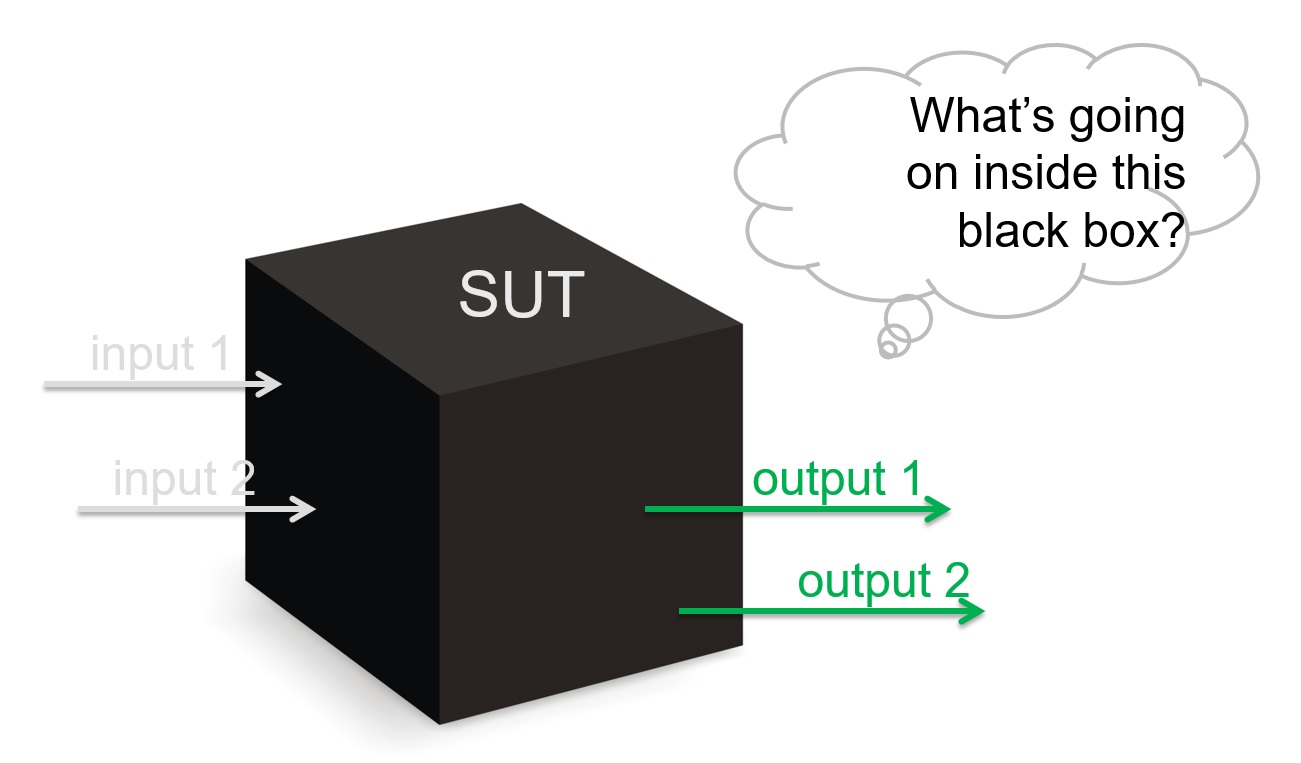
\includegraphics[width=.8\textwidth]{blackbox.jpg}
\end{center}

\pause
\red{We assume SUT behaves deterministically and can be reset.}
}

\frame{
	\frametitle{Machine Learning in General}
	
	\begin{center}
		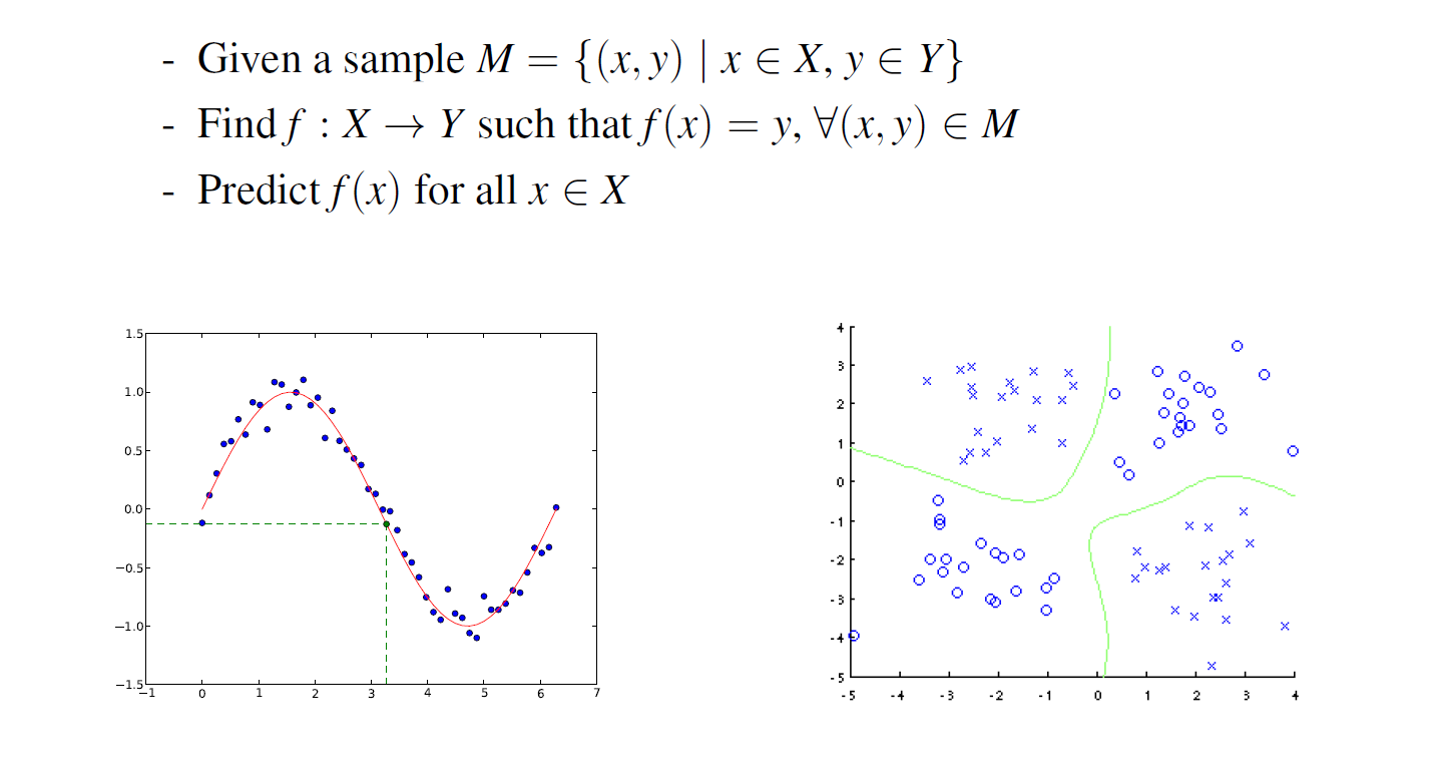
\includegraphics[width=\textwidth]{machinelearningingeneral.png}
	\end{center}
}

\frame{
	\frametitle{Learning Regular Languages}
	
	\begin{center}
		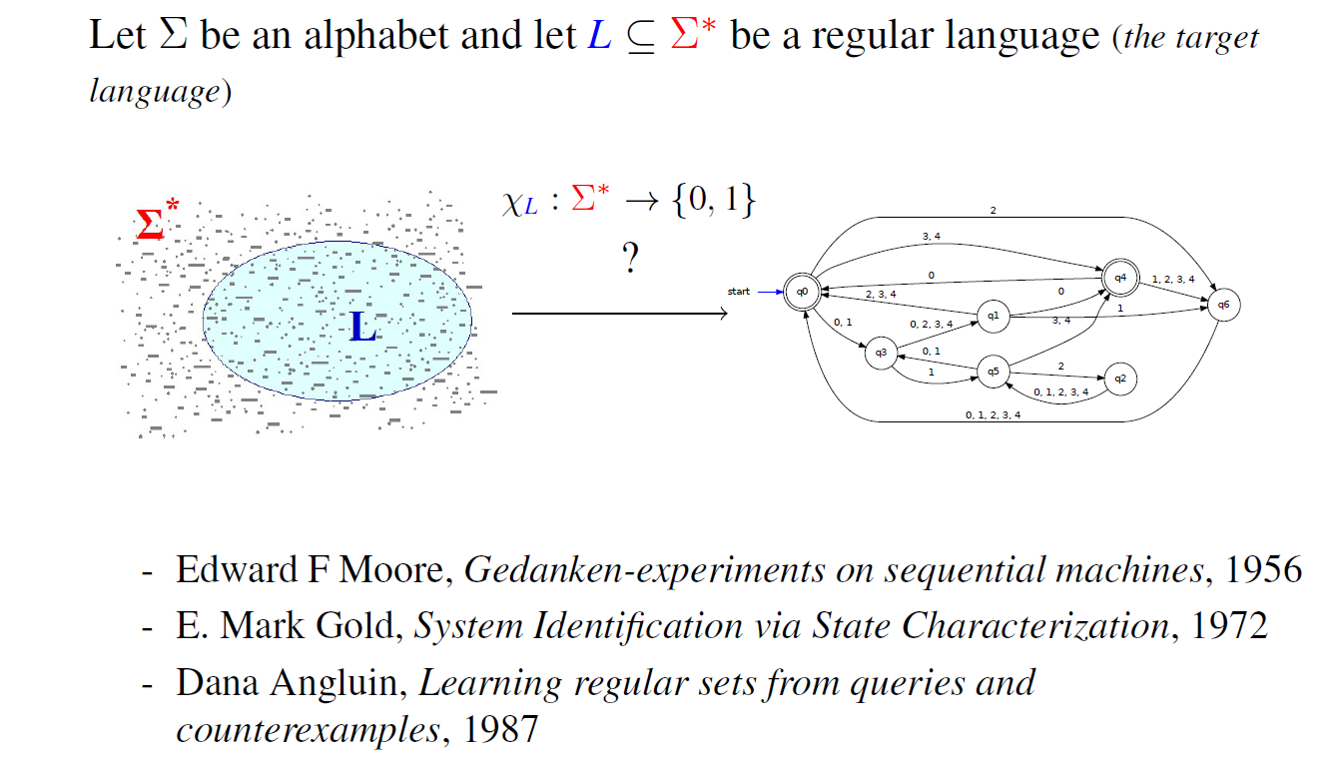
\includegraphics[width=\textwidth]{learningregularlanguages.png}
	\end{center}
}

\frame{
\frametitle{Regular Languages and Congruences}

\begin{definition}
The equivalence relation \red{$\sim_L$}\  on $\Sigma^{\ast}$ induced by a language $L \subseteq \Sigma^{\ast}$:
\begin{eqnarray*}
	u \sim_L v & iff  & \forall w \in \Sigma^{\ast} : u \cdot w \in L \Leftrightarrow v \cdot w \in L
\end{eqnarray*}
\end{definition}

This relation is a right-congruence with respect to concatenation:
\[
\forall u, v, w \in \Sigma^{\ast} : u \sim_L v \Rightarrow u \cdot w \sim_L v \cdot w
\]

\begin{theorem}[Myhill-Nerode, 1958]
	Language $L$ is regular iff $\sim_L$ has finitely equivalence classes.
\end{theorem}
}
\frame{
\frametitle{Visualisation}
Consider the regular language \green{$a (a \mid b)^{\ast} b$}
	
	\begin{center}
		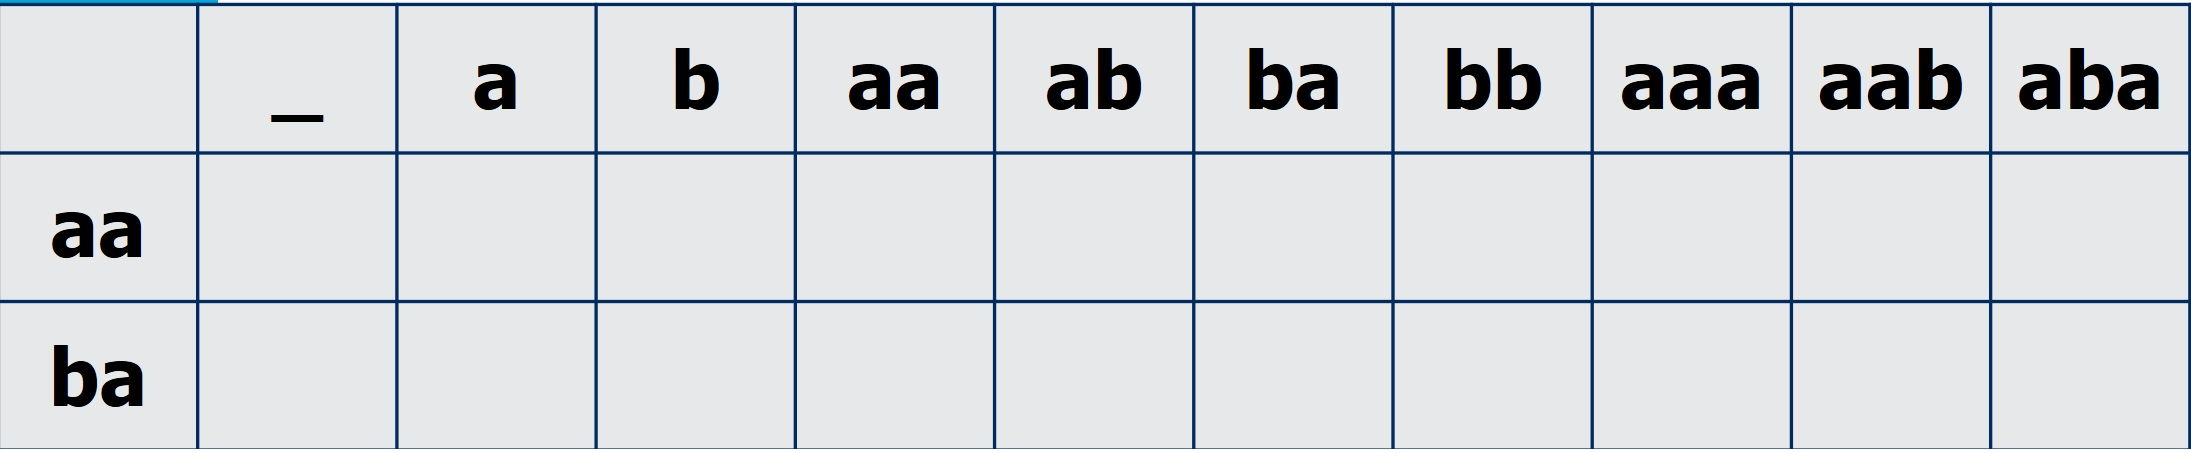
\includegraphics[width=\textwidth]{matrix1.jpg}
	\end{center}
}

\frame{
\frametitle{Visualisation}
Consider the regular language \green{$a (a \mid b)^{\ast} b$}
	
	\begin{center}
		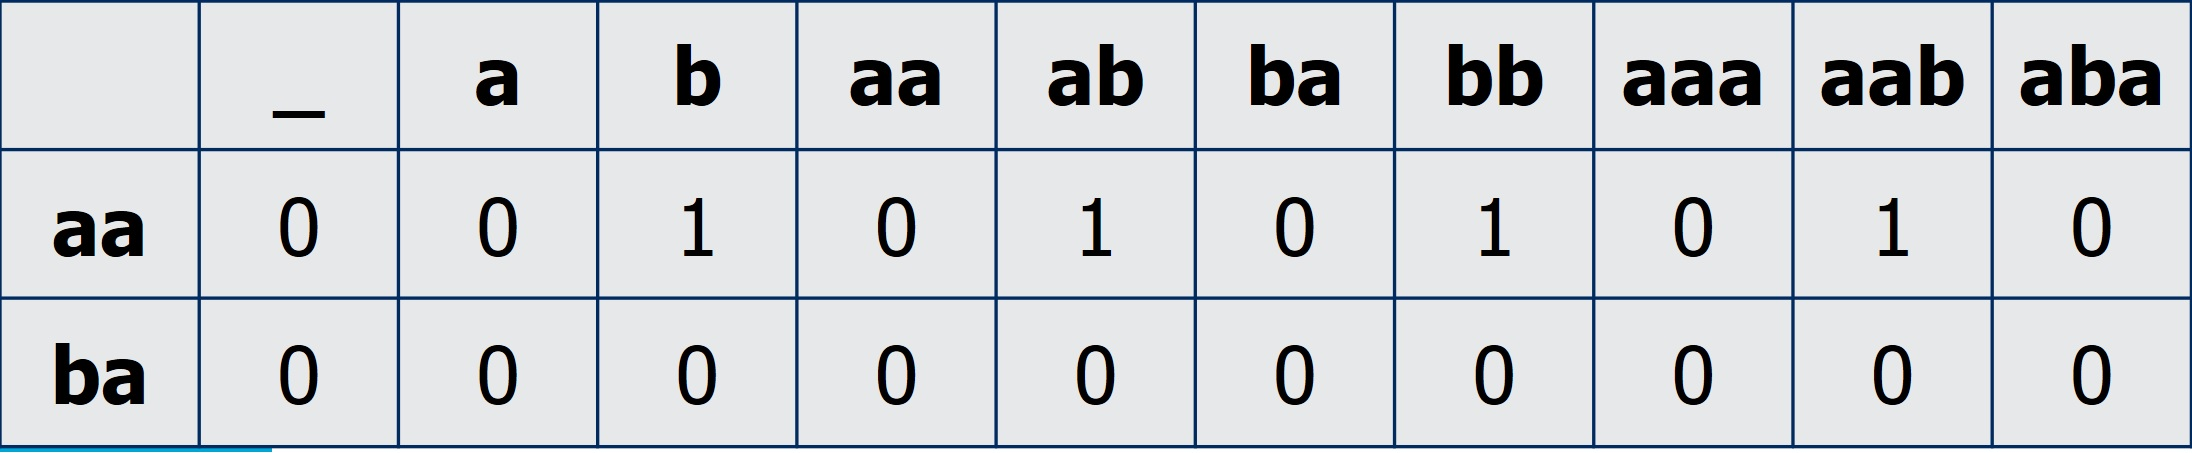
\includegraphics[width=\textwidth]{matrix2.jpg}
	\end{center}
}

\frame{
\frametitle{Hankel Matrix}
	
	\begin{center}
		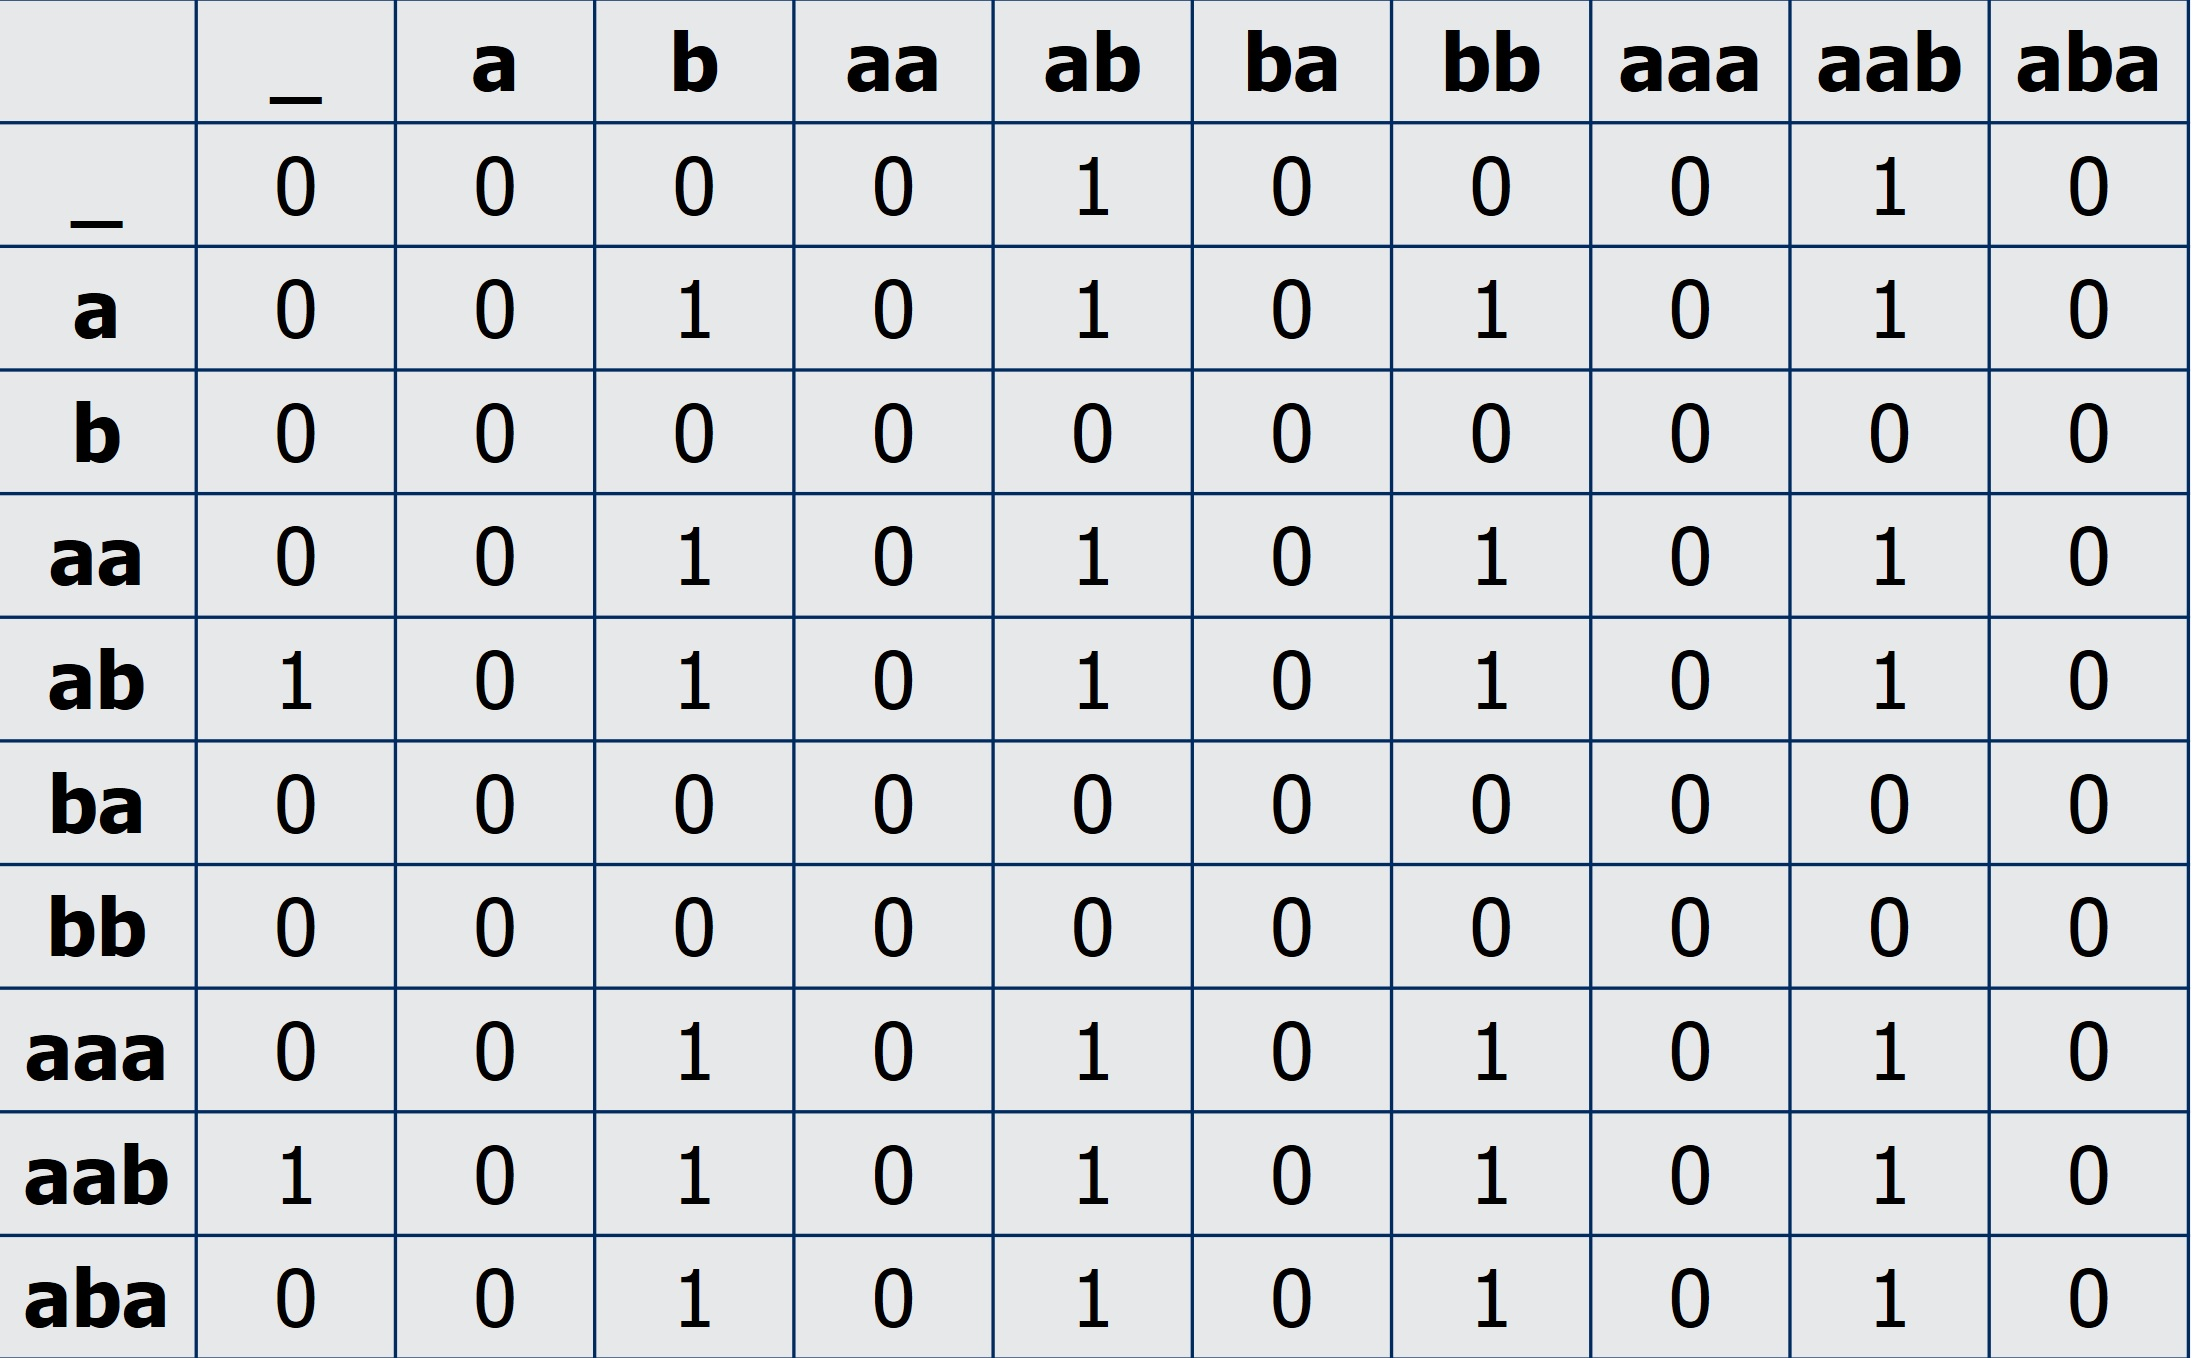
\includegraphics[width=\textwidth]{matrix3.jpg}
	\end{center}
}

\frame{
\frametitle{Hankel Matrix}
	
	\begin{center}
		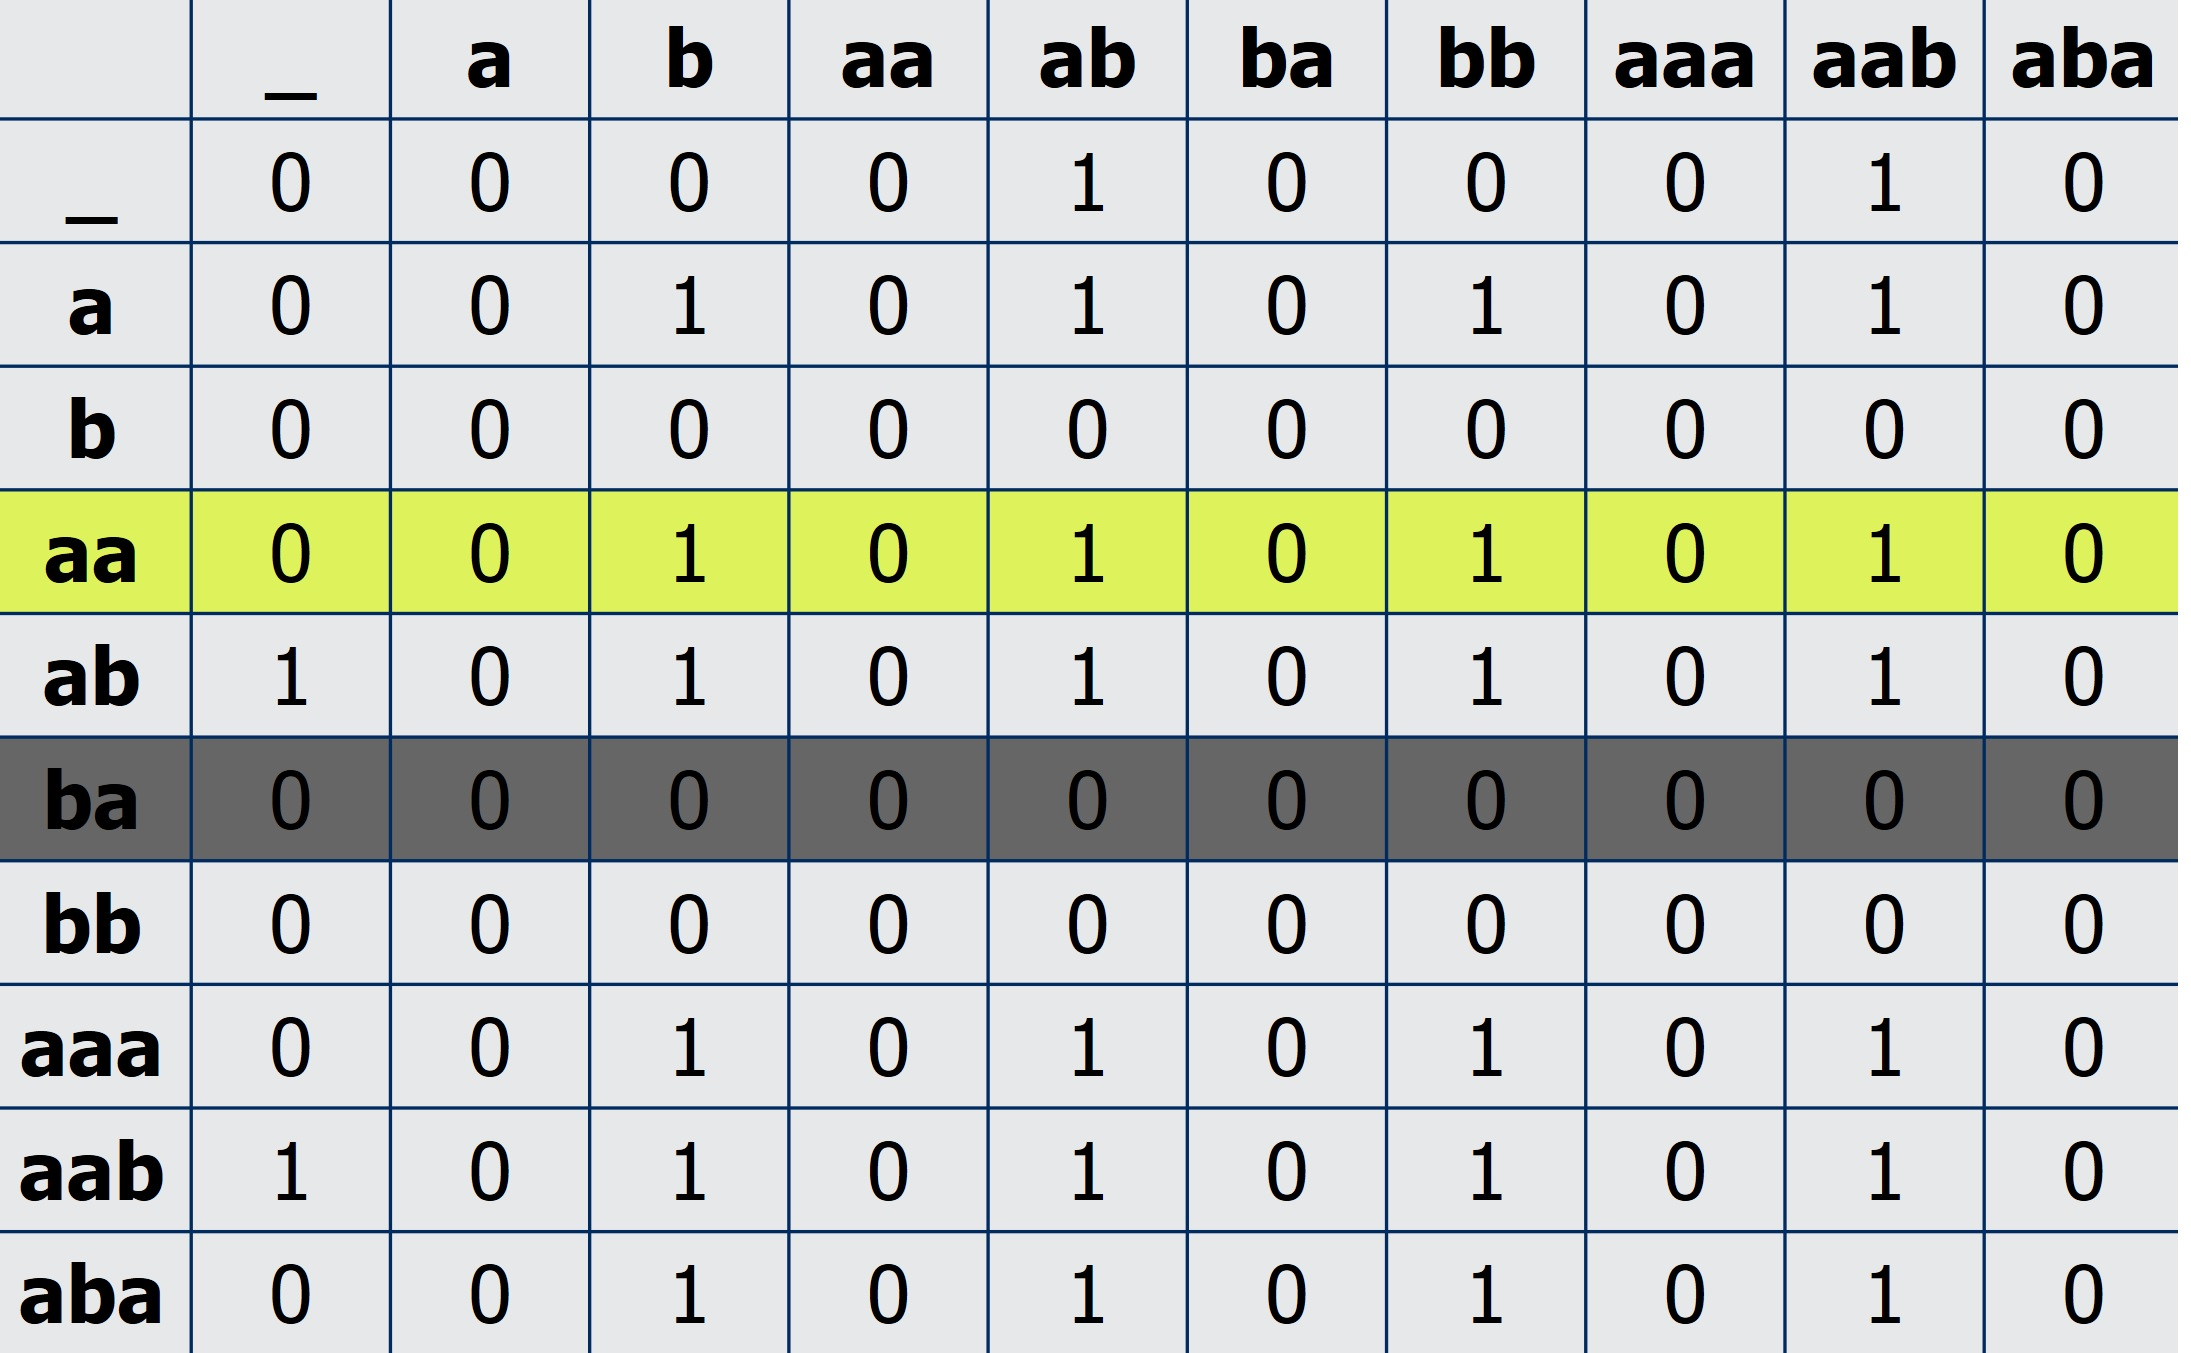
\includegraphics[width=\textwidth]{matrix4.jpg}
	\end{center}
}

\frame{
\frametitle{Hankel Matrix}
	
	\begin{center}
		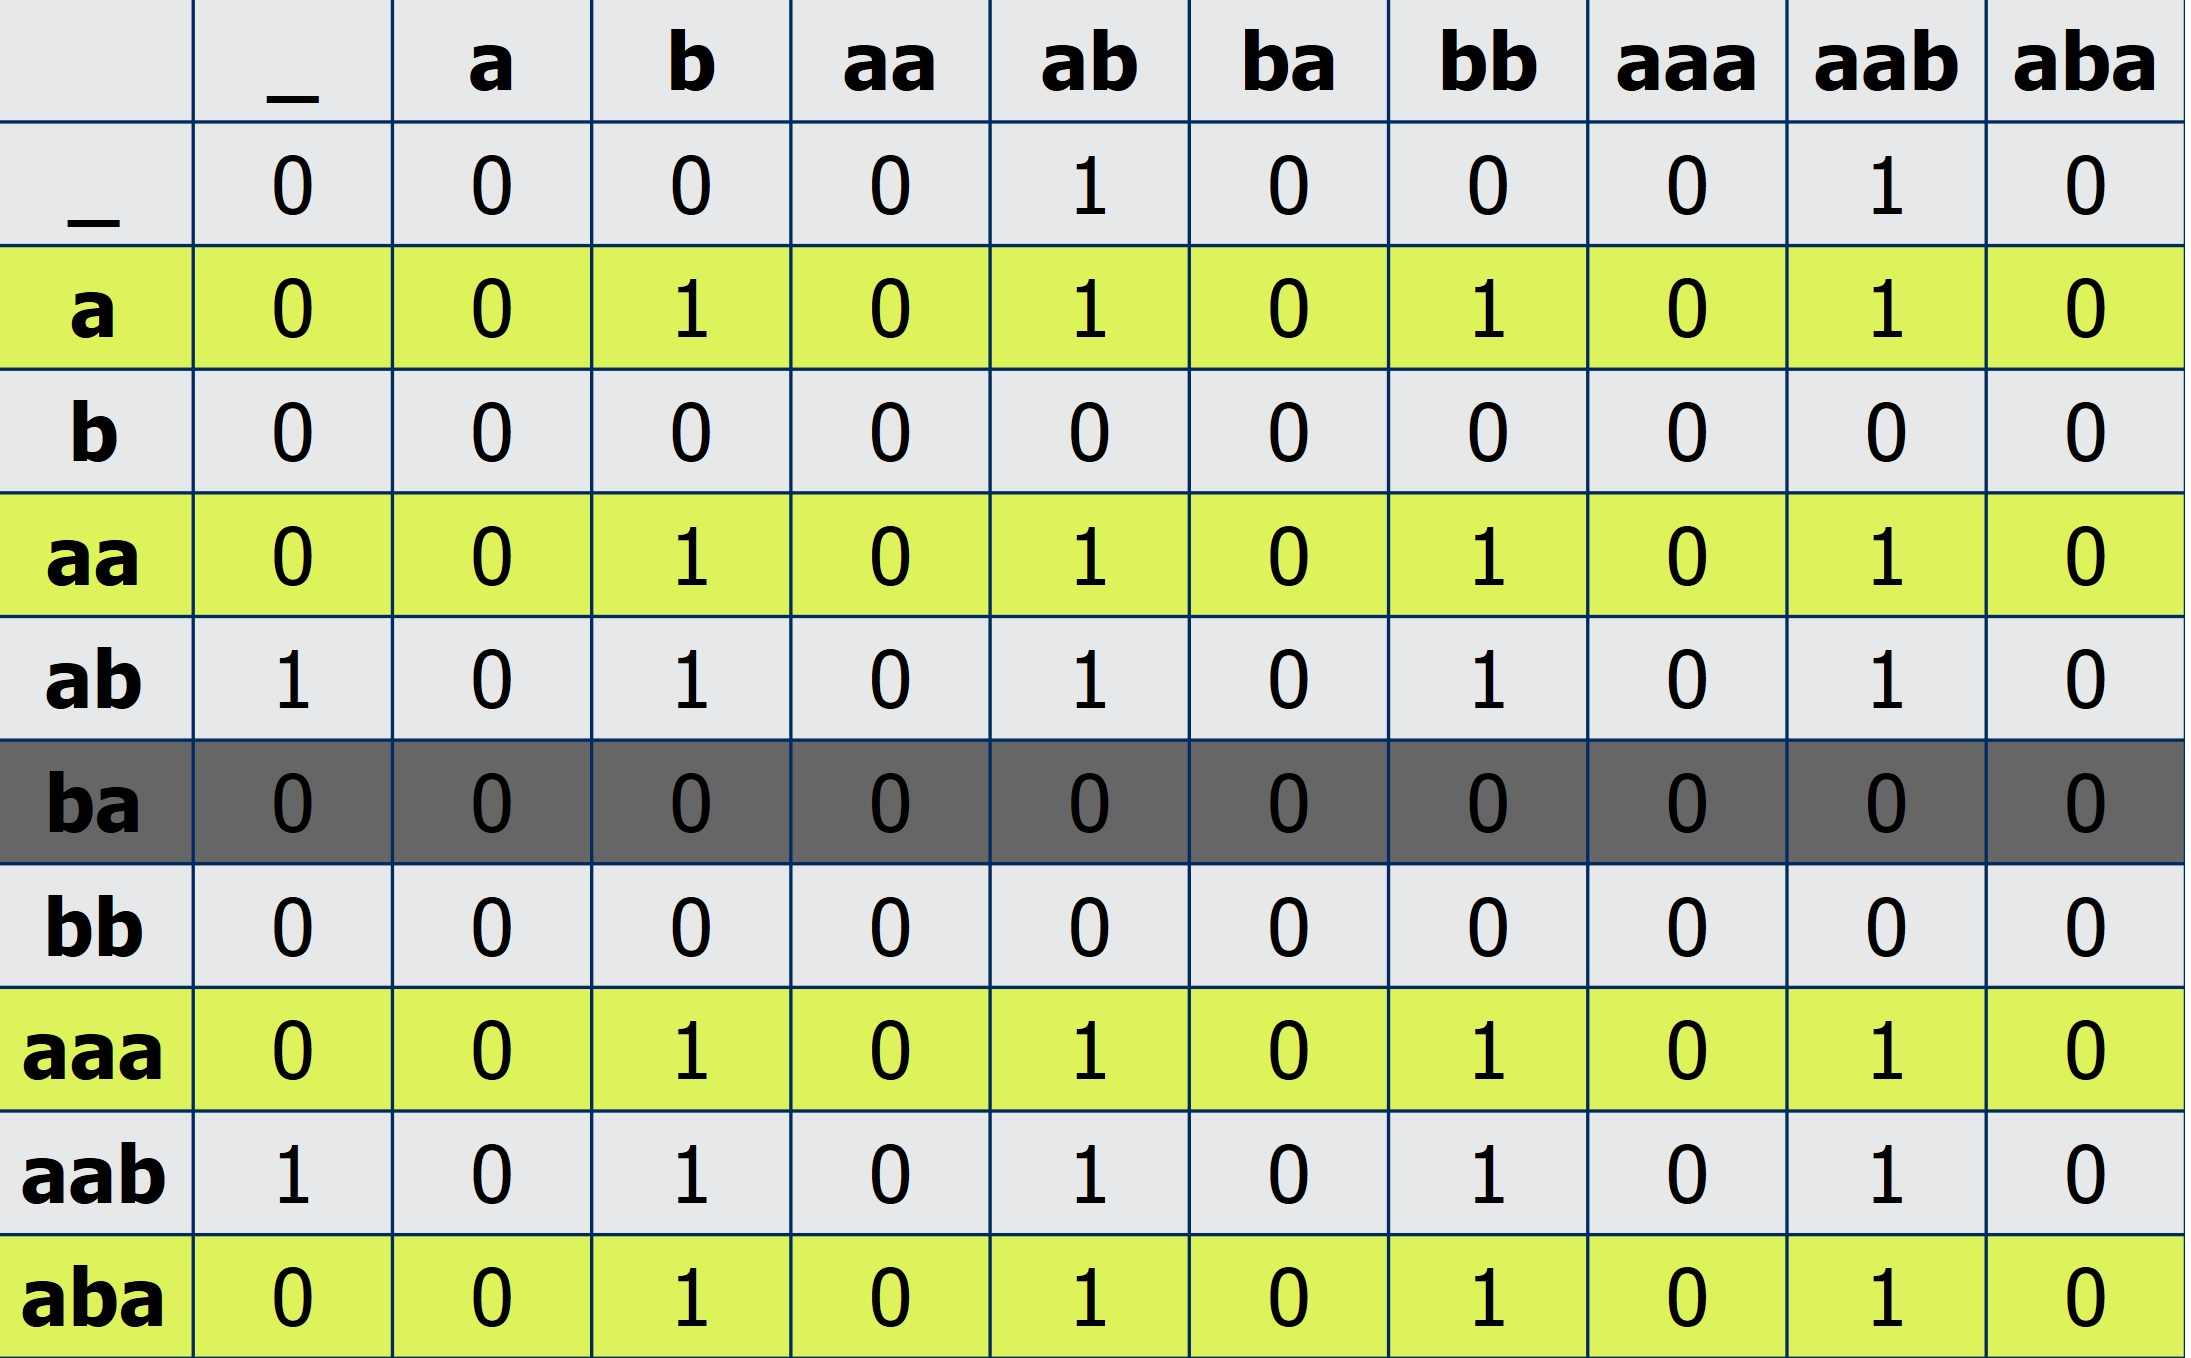
\includegraphics[width=\textwidth]{matrix5.jpg}
	\end{center}
}

\frame{
\frametitle{Hankel Matrix}
	
	\begin{center}
		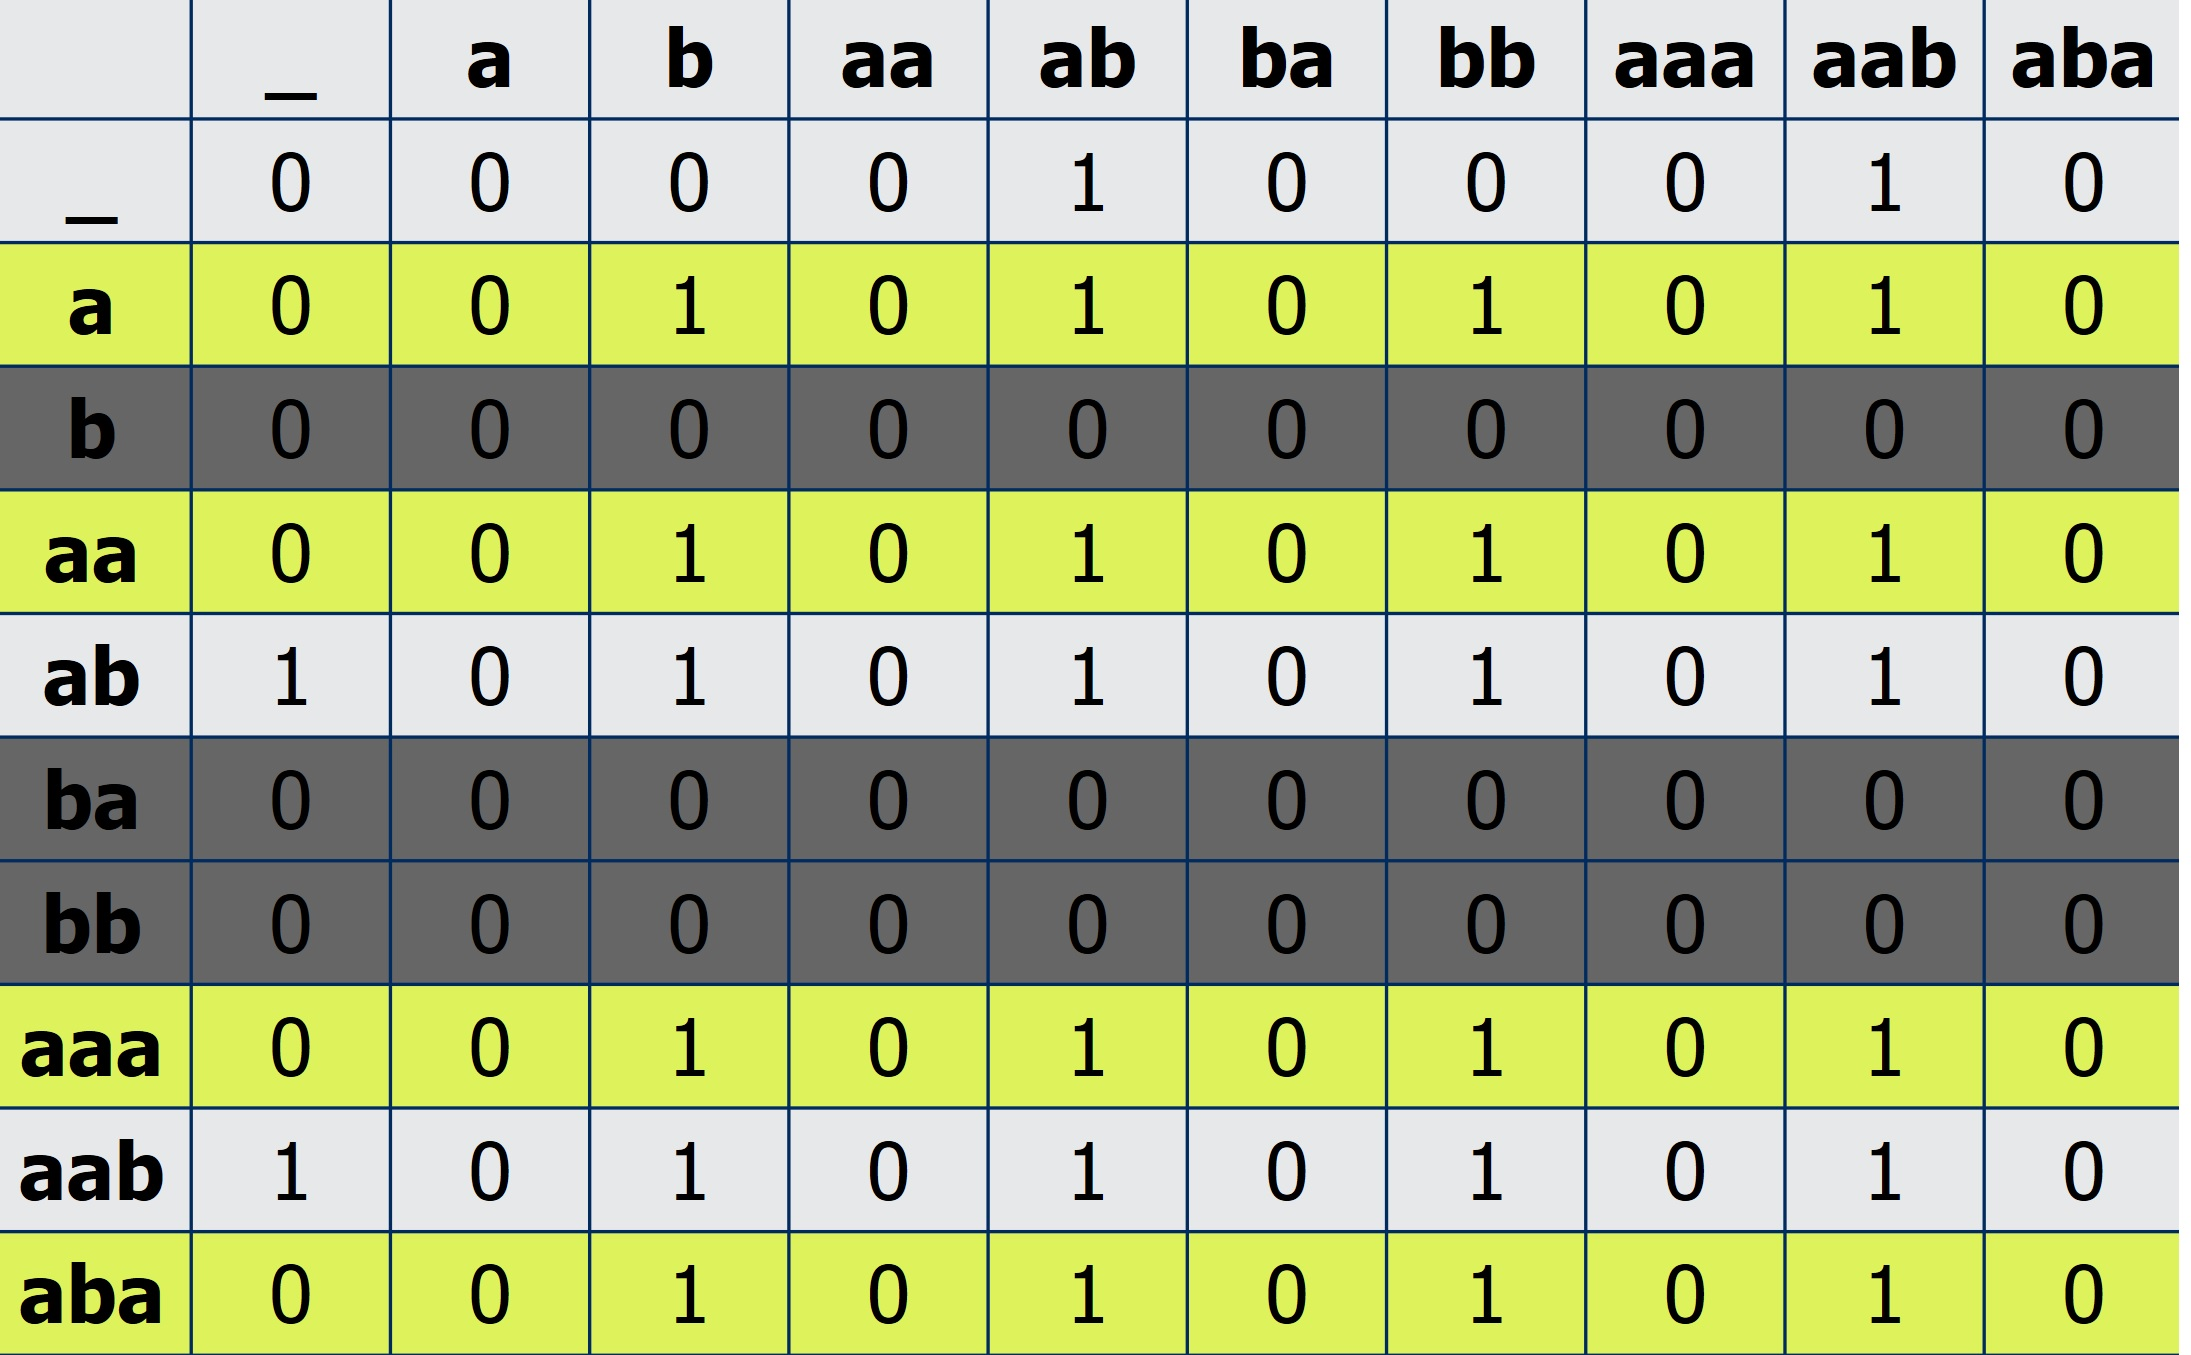
\includegraphics[width=\textwidth]{matrix6.jpg}
	\end{center}
}

\frame{
\frametitle{Hankel Matrix}
	
	\begin{center}
		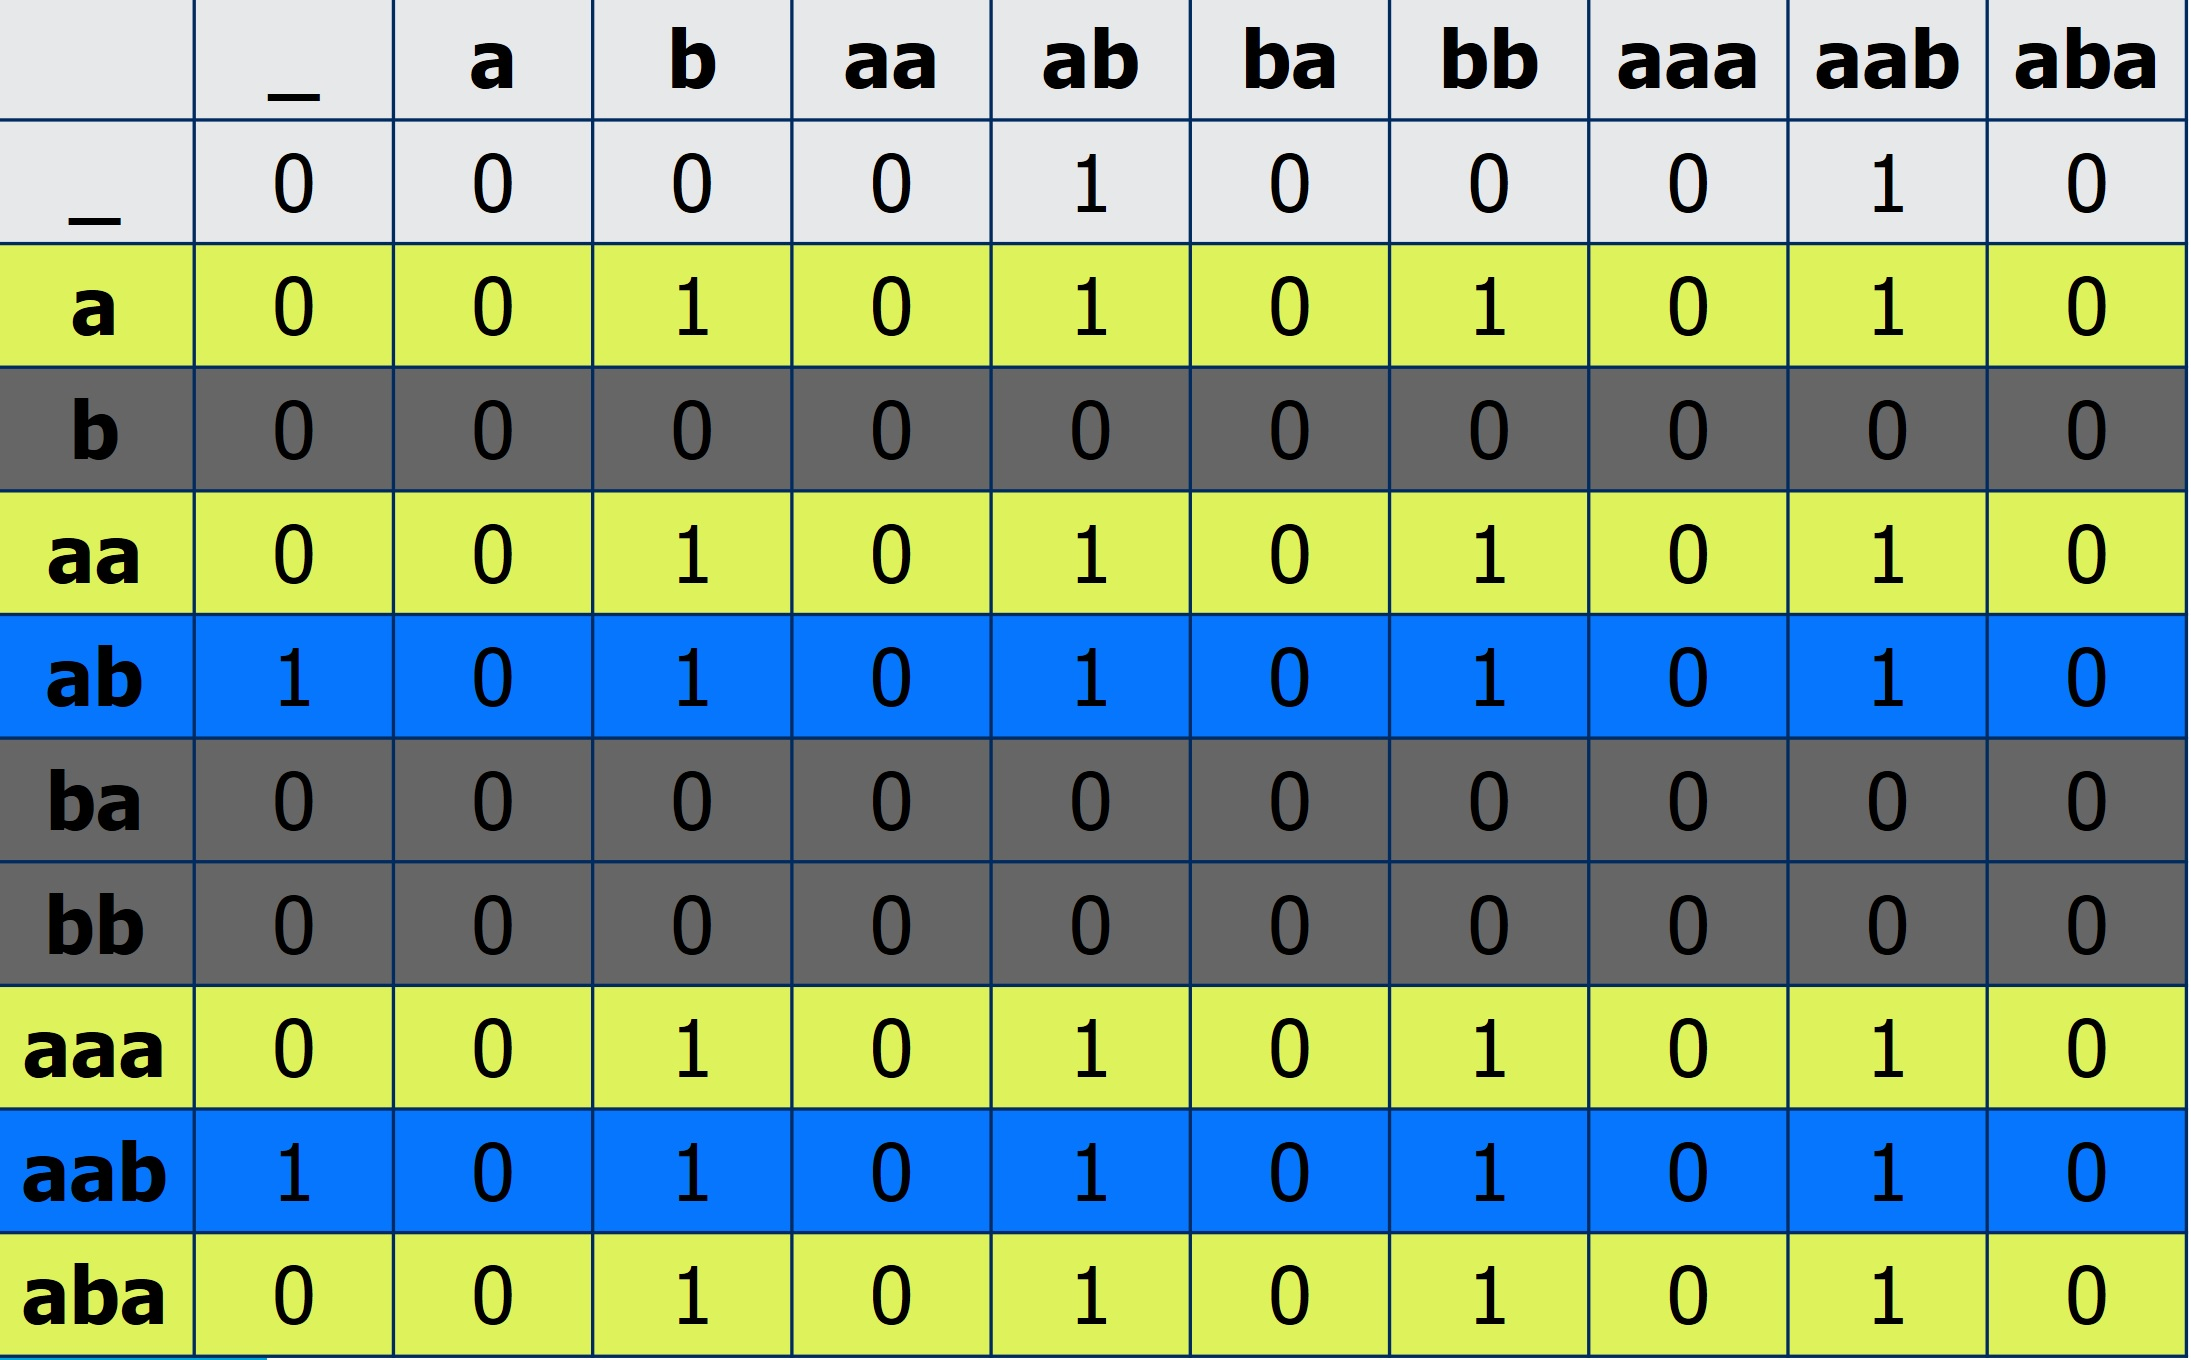
\includegraphics[width=\textwidth]{matrix7.jpg}
	\end{center}
}


\frame{
\frametitle{Hankel Matrix}	
	\begin{center}
		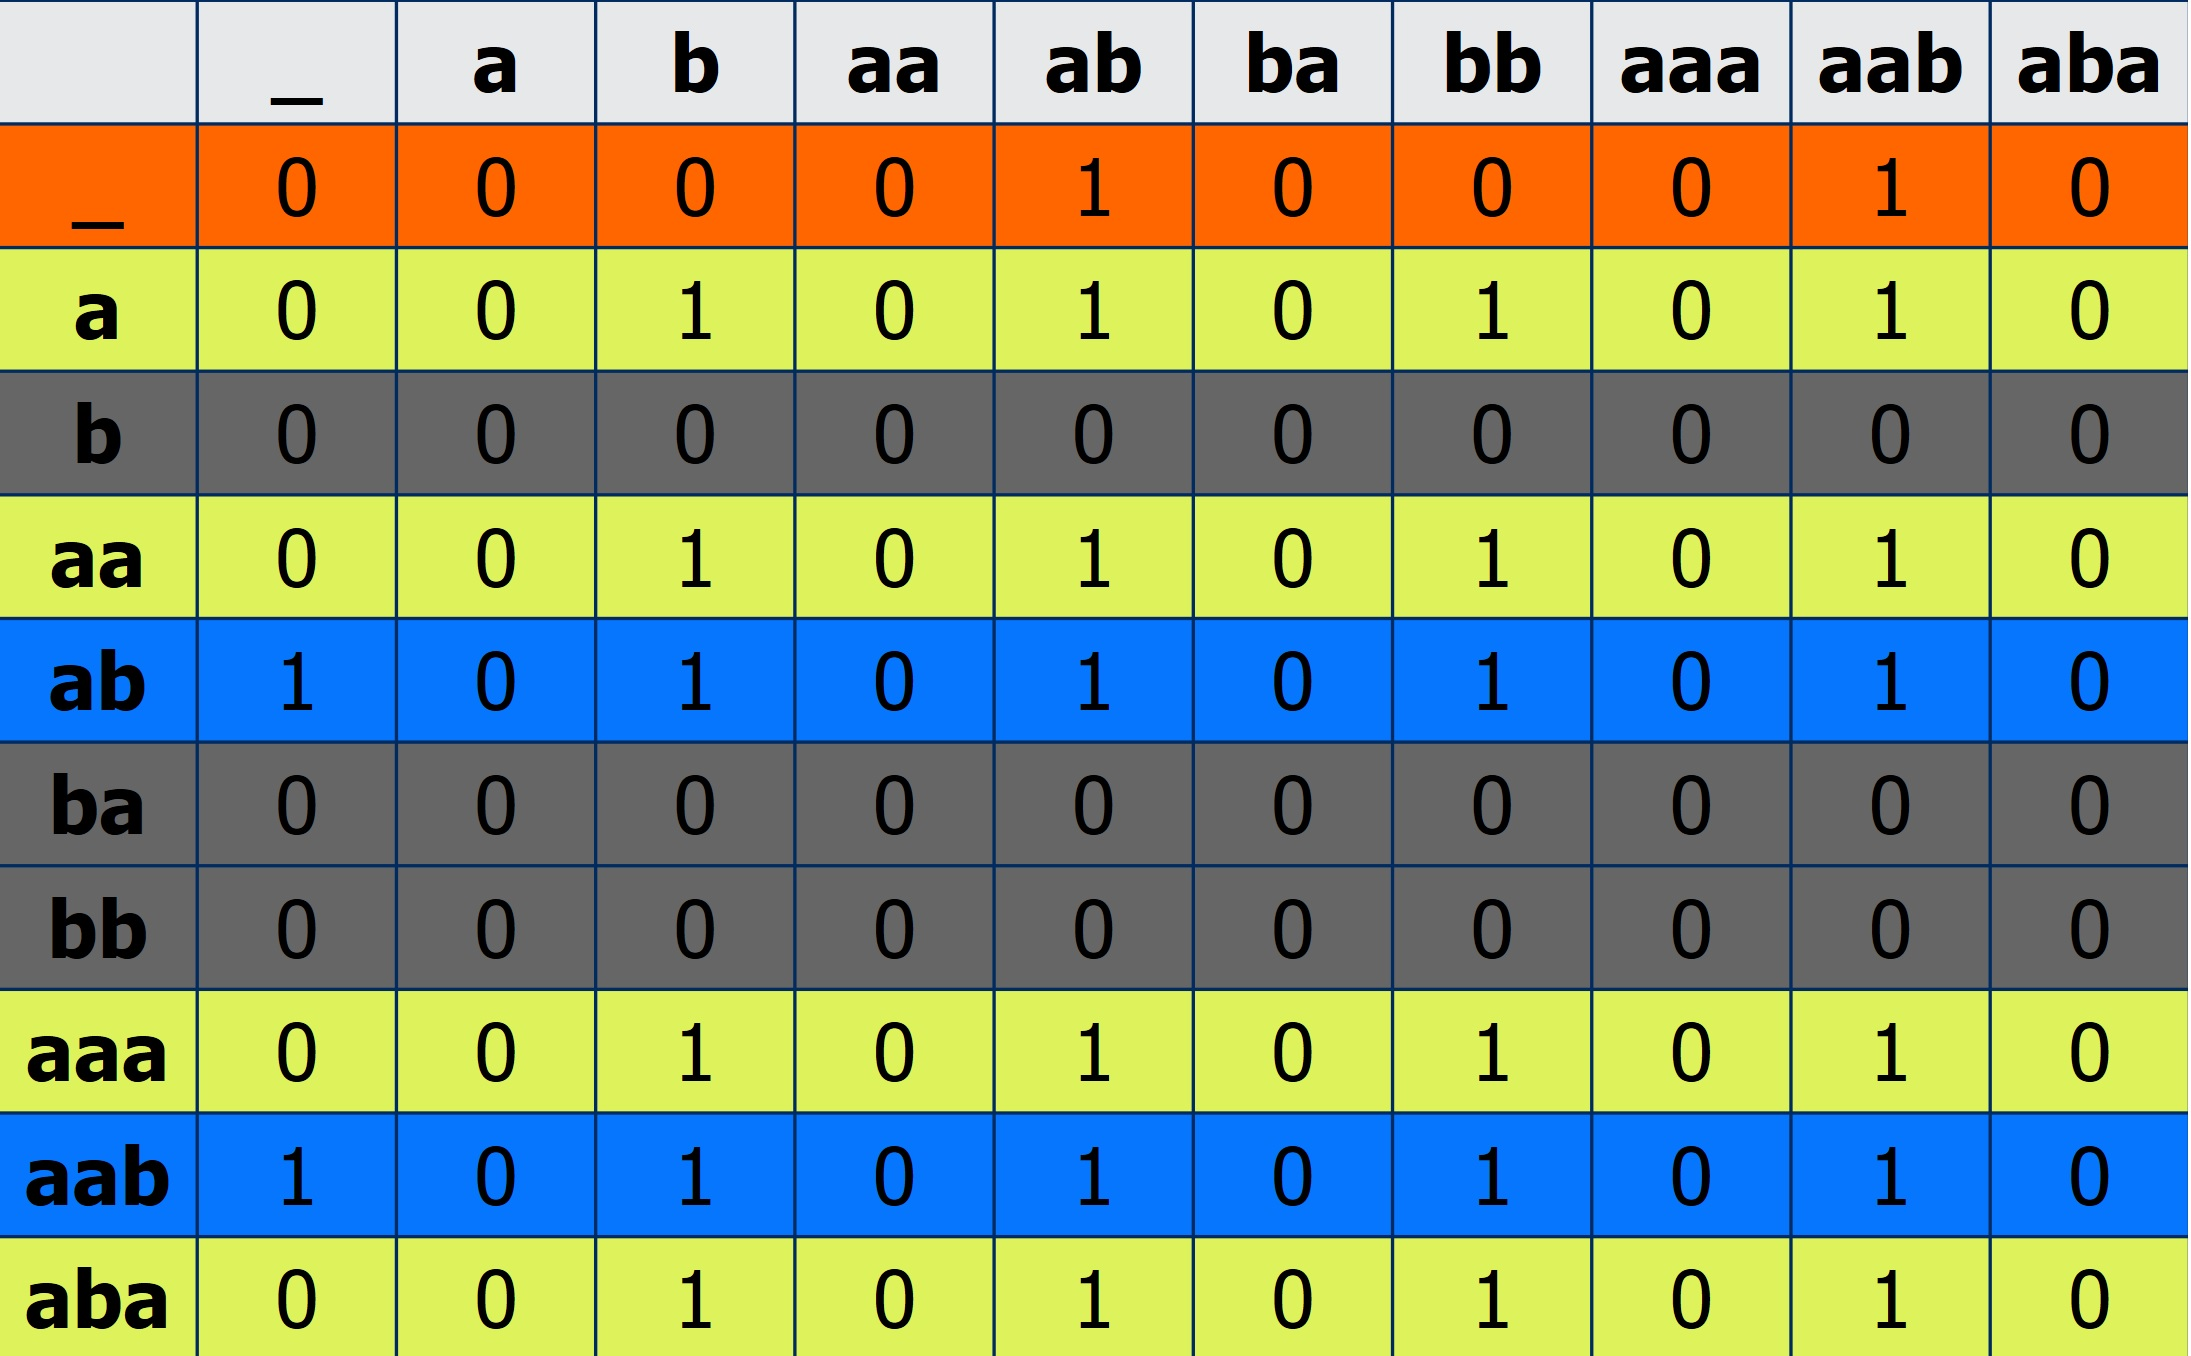
\includegraphics[width=\textwidth]{matrix8.jpg}
	\end{center}
}



\frame{
	\frametitle{Hankel Matrix}
\begin{itemize}
	\item 
	
	$u \sim_L v$ iff rows of $u$ and $v$ in Hankel matrix for $L$ have the same color
\pause	
\item
	Language $L$ is regular iff its Hankel matrix contains a \red{finite number of distinct rows}, i.e., colors
\pause	
\item
	The number of states in the smallest DFA for $L$ equals \red{the number of colors in the Hankel matrix}
\end{itemize}	
}


\frame{
	\frametitle{What is the FSM for this Hankel Matrix?}
	
	\begin{center}
		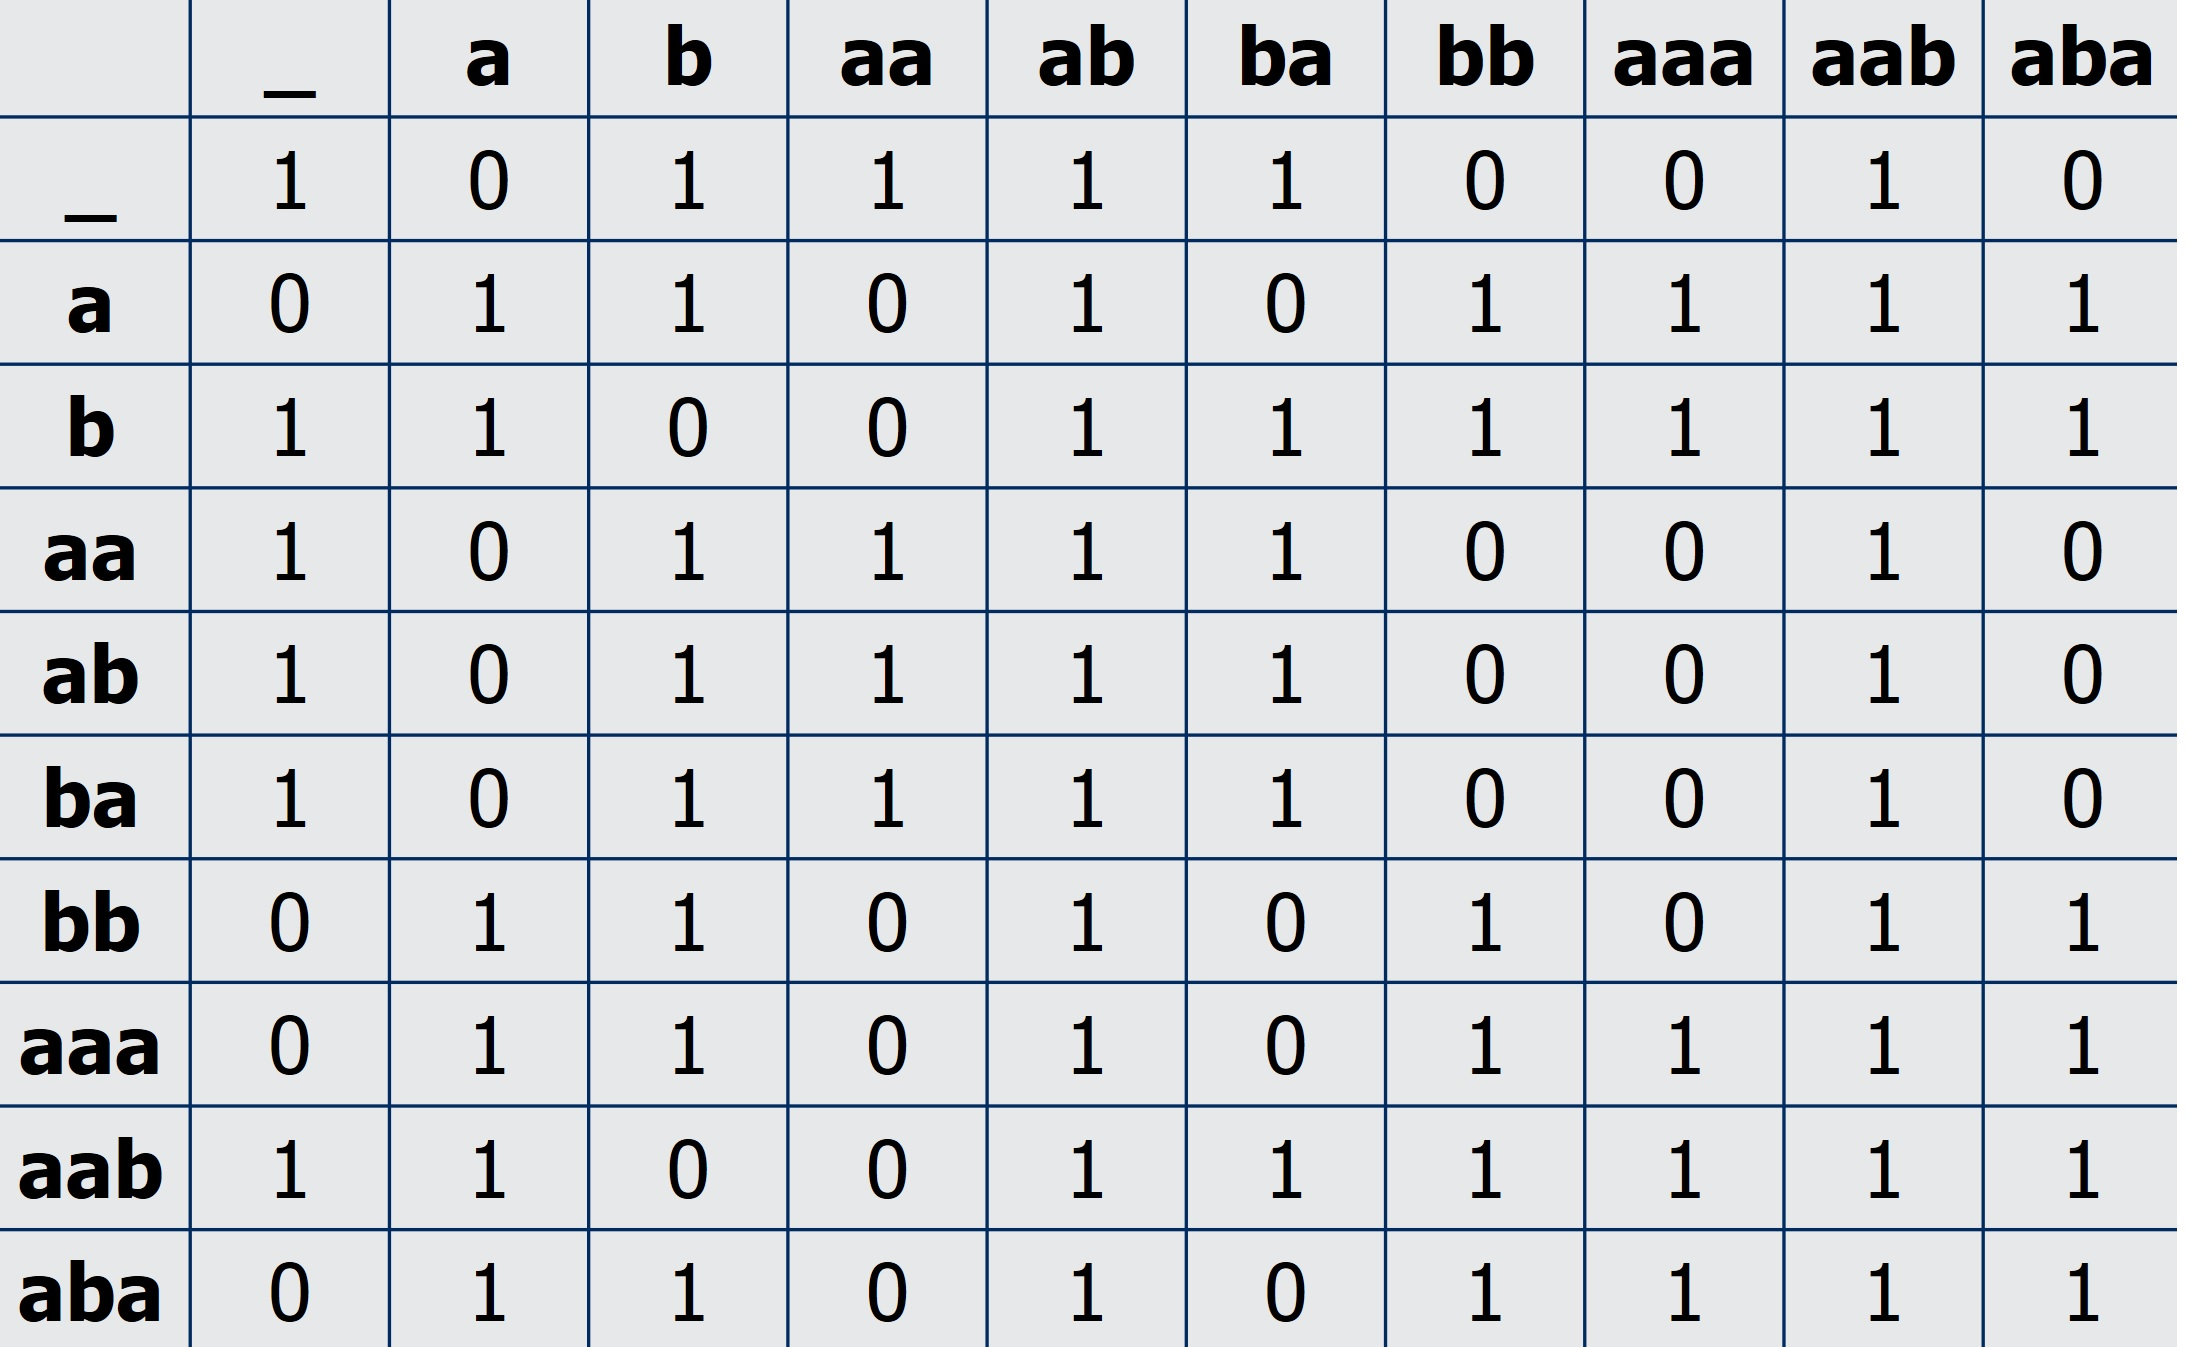
\includegraphics[width=\textwidth]{matrix9.jpg}
	\end{center}
}



\frame{
	\frametitle{What is the FSM for this Hankel Matrix?}	
	\begin{center}
		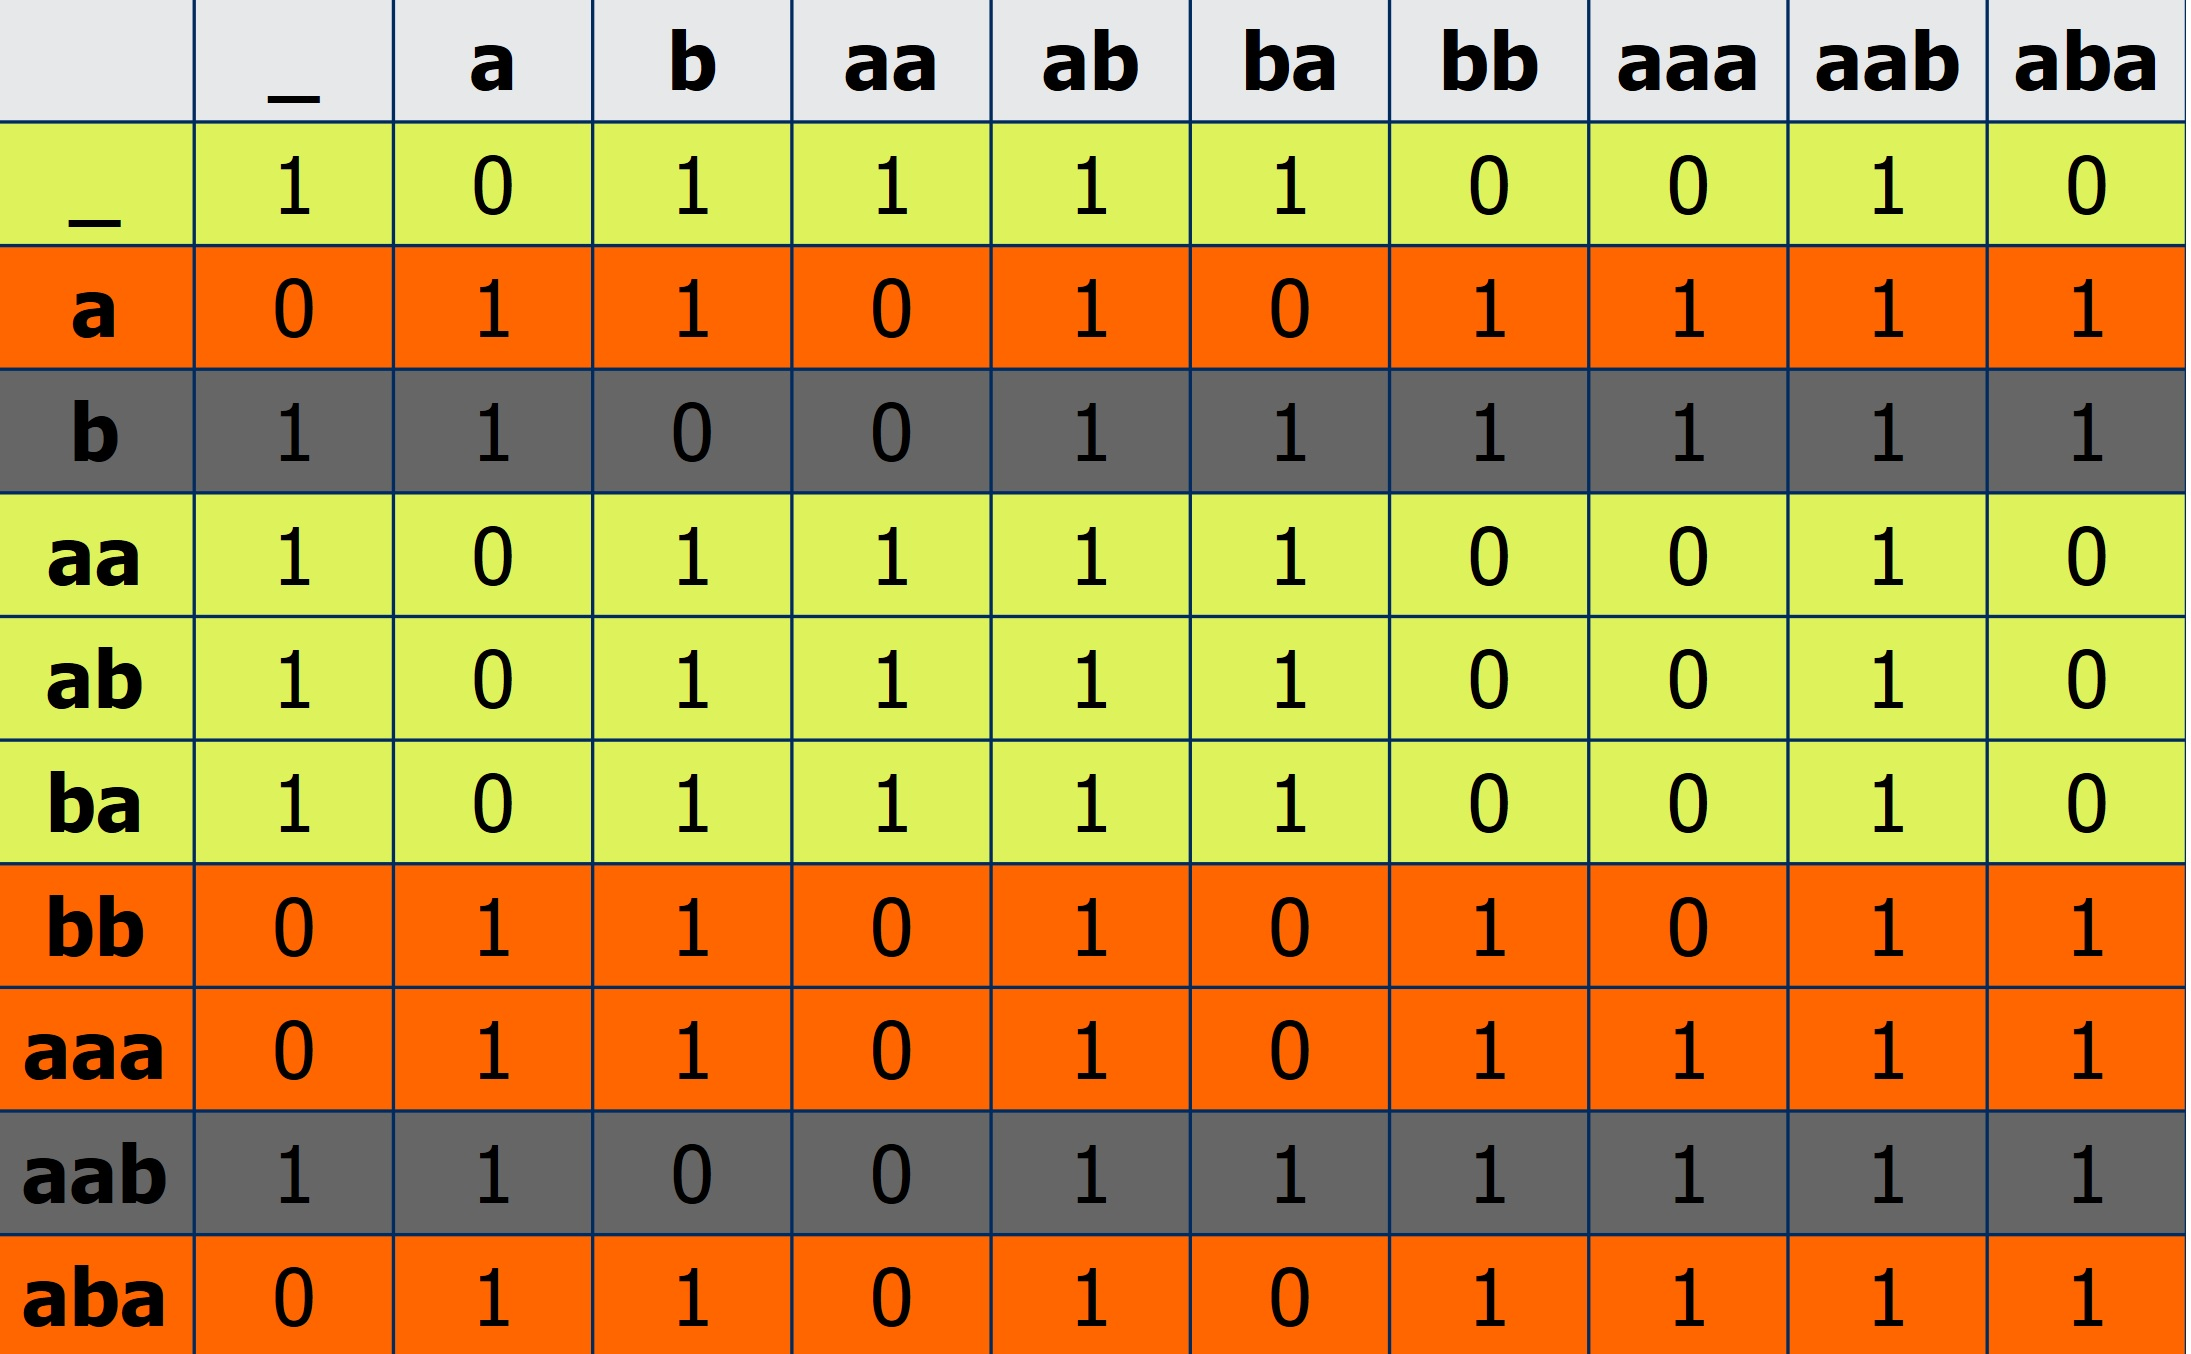
\includegraphics[width=\textwidth]{matrix10.jpg}
	\end{center}
}

\frame{
	\frametitle{Solution}
	\begin{center}
		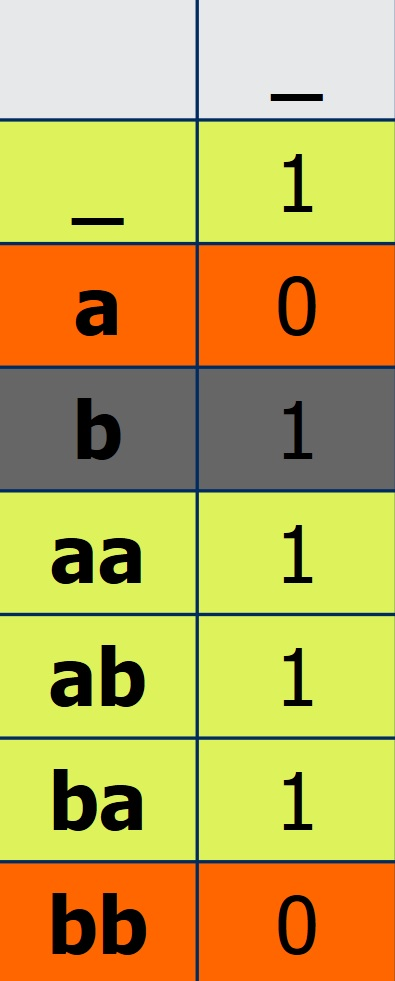
\includegraphics[width=1.5cm]{matrix11.jpg}
		\hspace{1cm}
		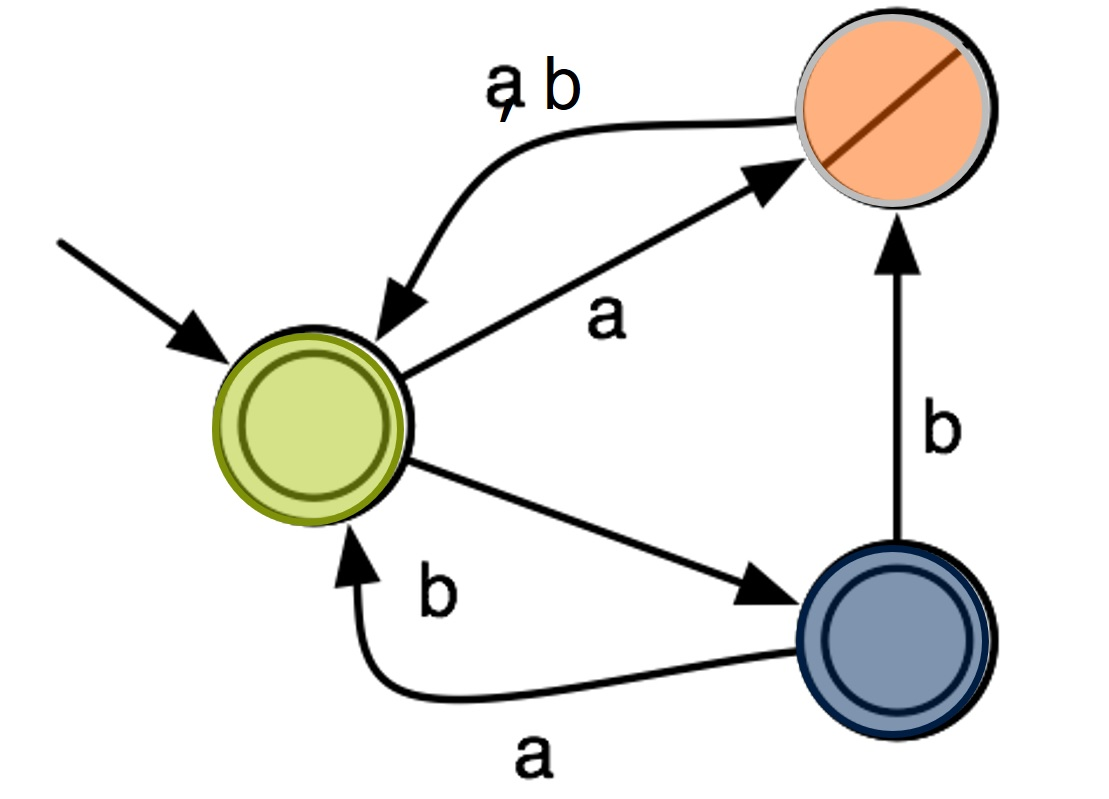
\includegraphics[width=5cm]{DFAsicco.jpg}
	\end{center}

Colors of rows in Hankel matrix give us the states.

Access strings and one-letter extensions allow us to determine transitions.

Column for empty suffix gives us the accepting states. 
}


\frame{
	\frametitle{What if Hankel Matrix is Incomplete?}	
	\begin{center}
		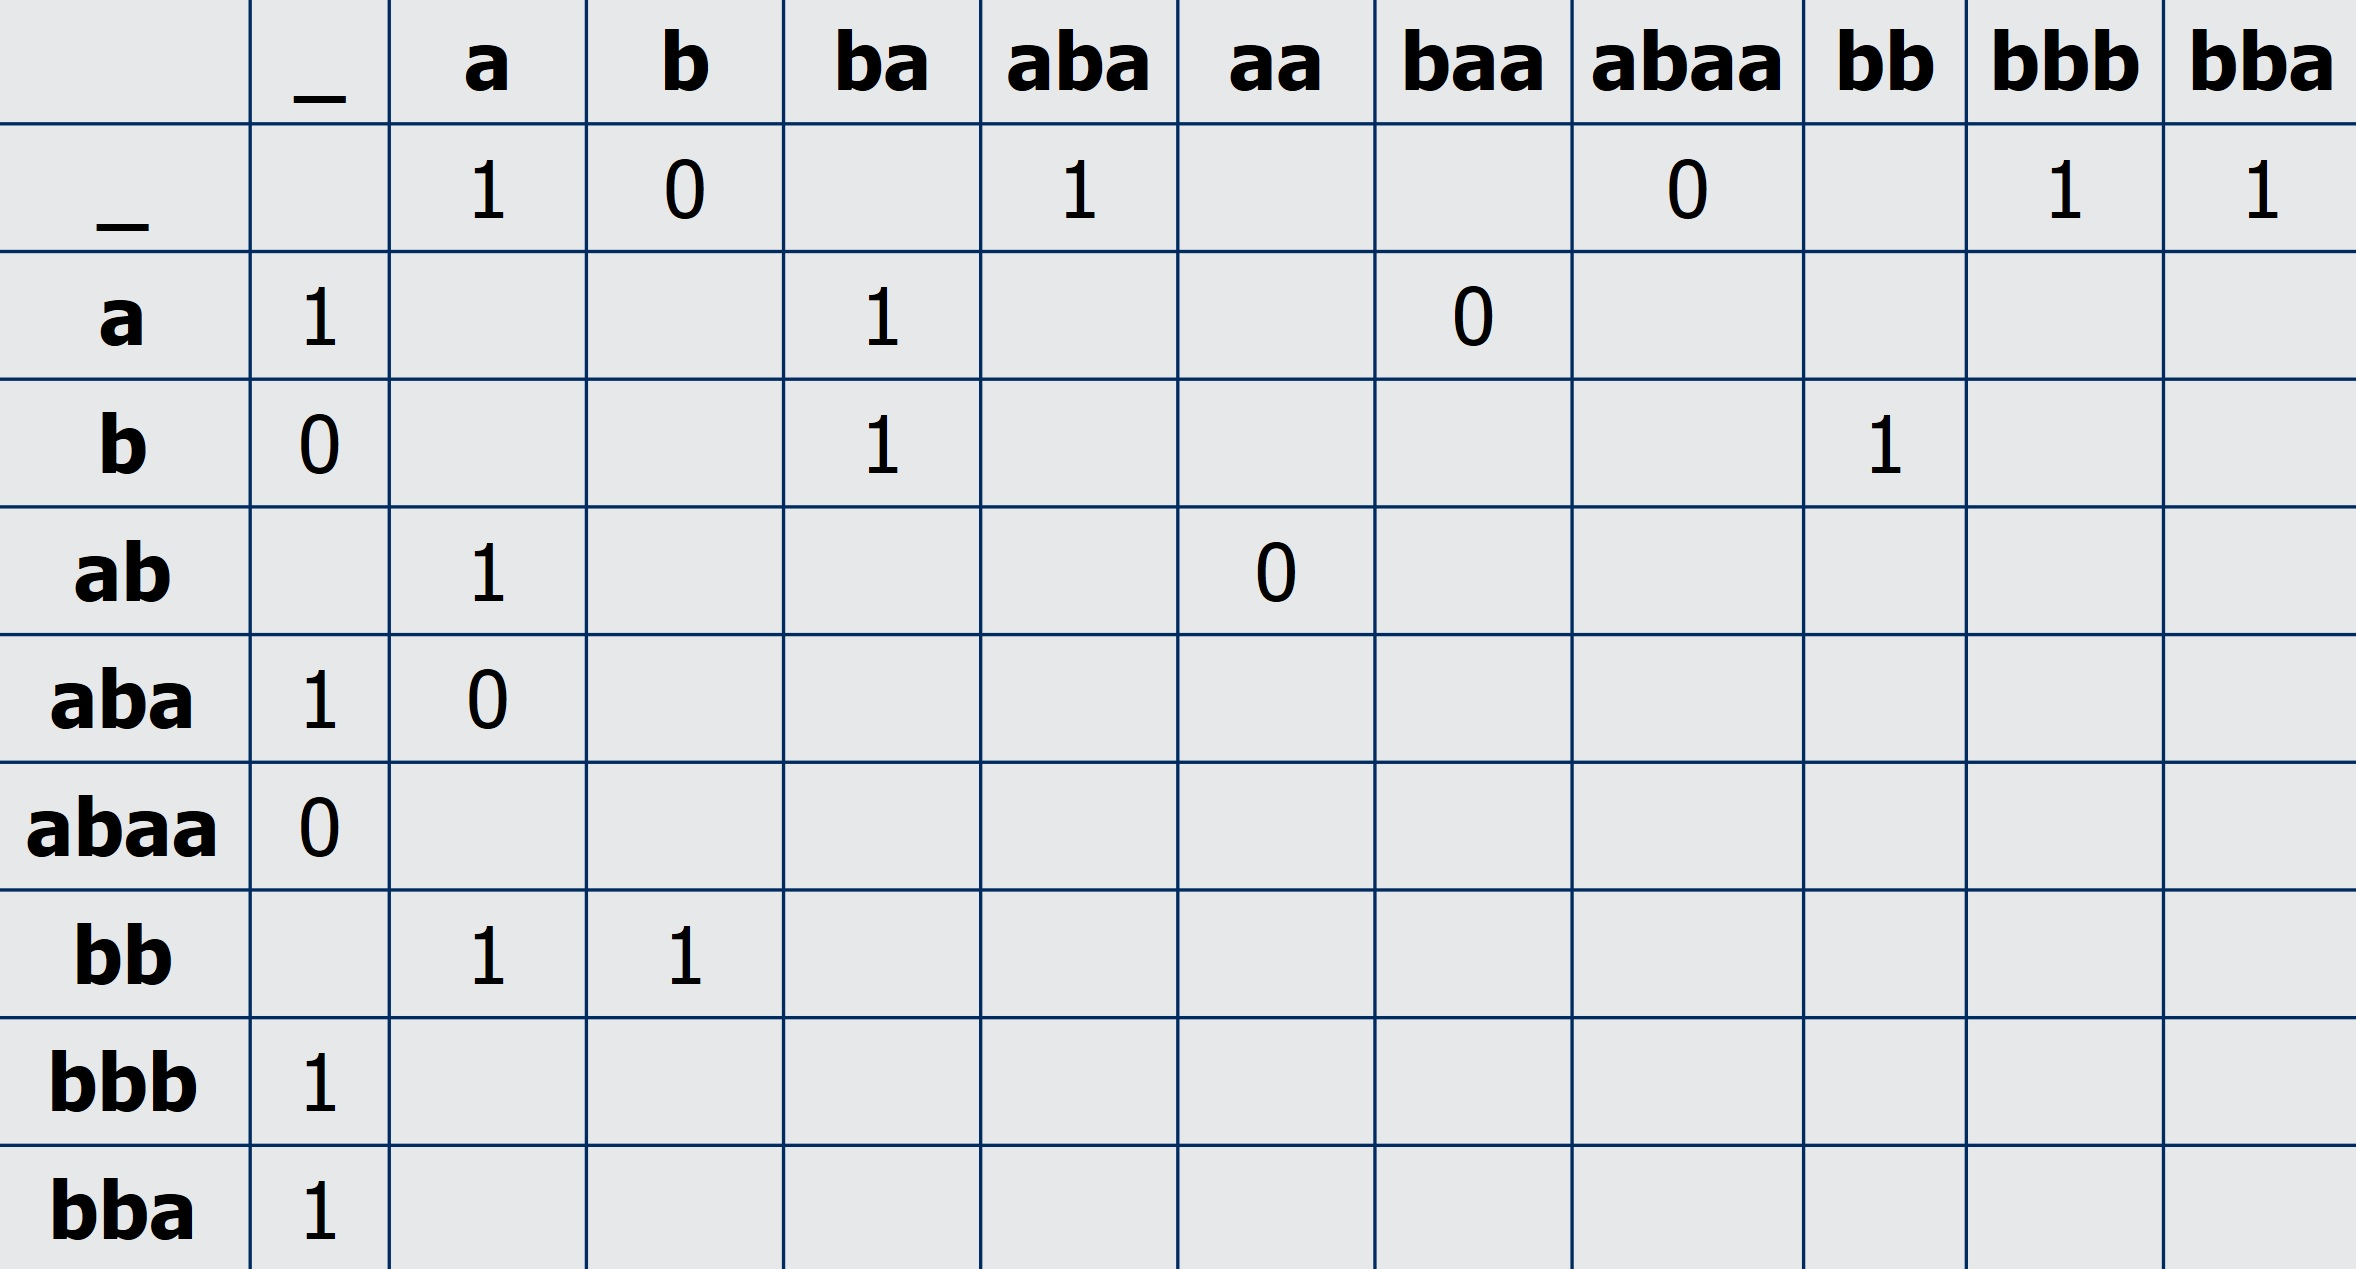
\includegraphics[width=\textwidth]{matrix12.jpg}
	\end{center}
\red{Problem to color such a matrix is NP-hard!}
}

\frame{
\frametitle{Minimally Adequate Teacher (Angluin)}

\begin{center}
	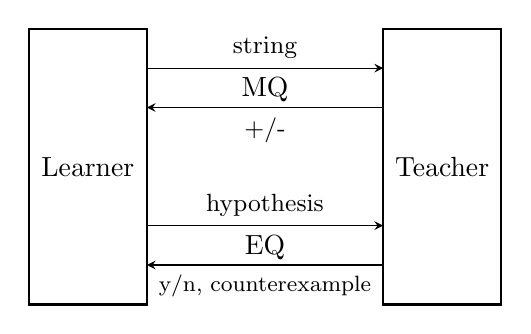
\begin{tikzpicture}[>=stealth]
	\draw [thick] (0,0) rectangle (1.5,3.5) node[midway] {Learner};
	\draw [thick] (4.5,0) rectangle (6,3.5) node[midway] {Teacher};
	\draw [->] (1.5,3) -- (4.5,3) node[midway,below] {MQ};
	\draw (1.5,3) -- (4.5,3) node[midway,above] {\small string};
	\draw [<-] (1.5,2.5) -- (4.5,2.5) node[midway,below] {\small +/-};
	\draw [->] (1.5,1) -- (4.5,1) node[midway,below] {EQ};
	\draw (1.5,1) -- (4.5,1) node[midway,above] {\small hypothesis};
	\draw [<-] (1.5,0.5) -- (4.5,0.5) node[midway,below] {\footnotesize y/n, counterexample};
	\end{tikzpicture}
	\hspace{2 em}
	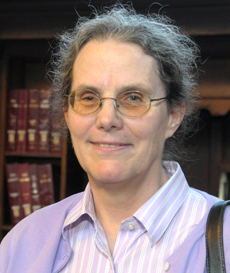
\includegraphics[width=.25\textwidth]{angluin.png}
\end{center}

Learner asks \red{membership queries}\ and \red{equivalence queries}
}

\frame{
\frametitle{Angluin's $L^{\ast}$ Algorithm}

\begin{center}
	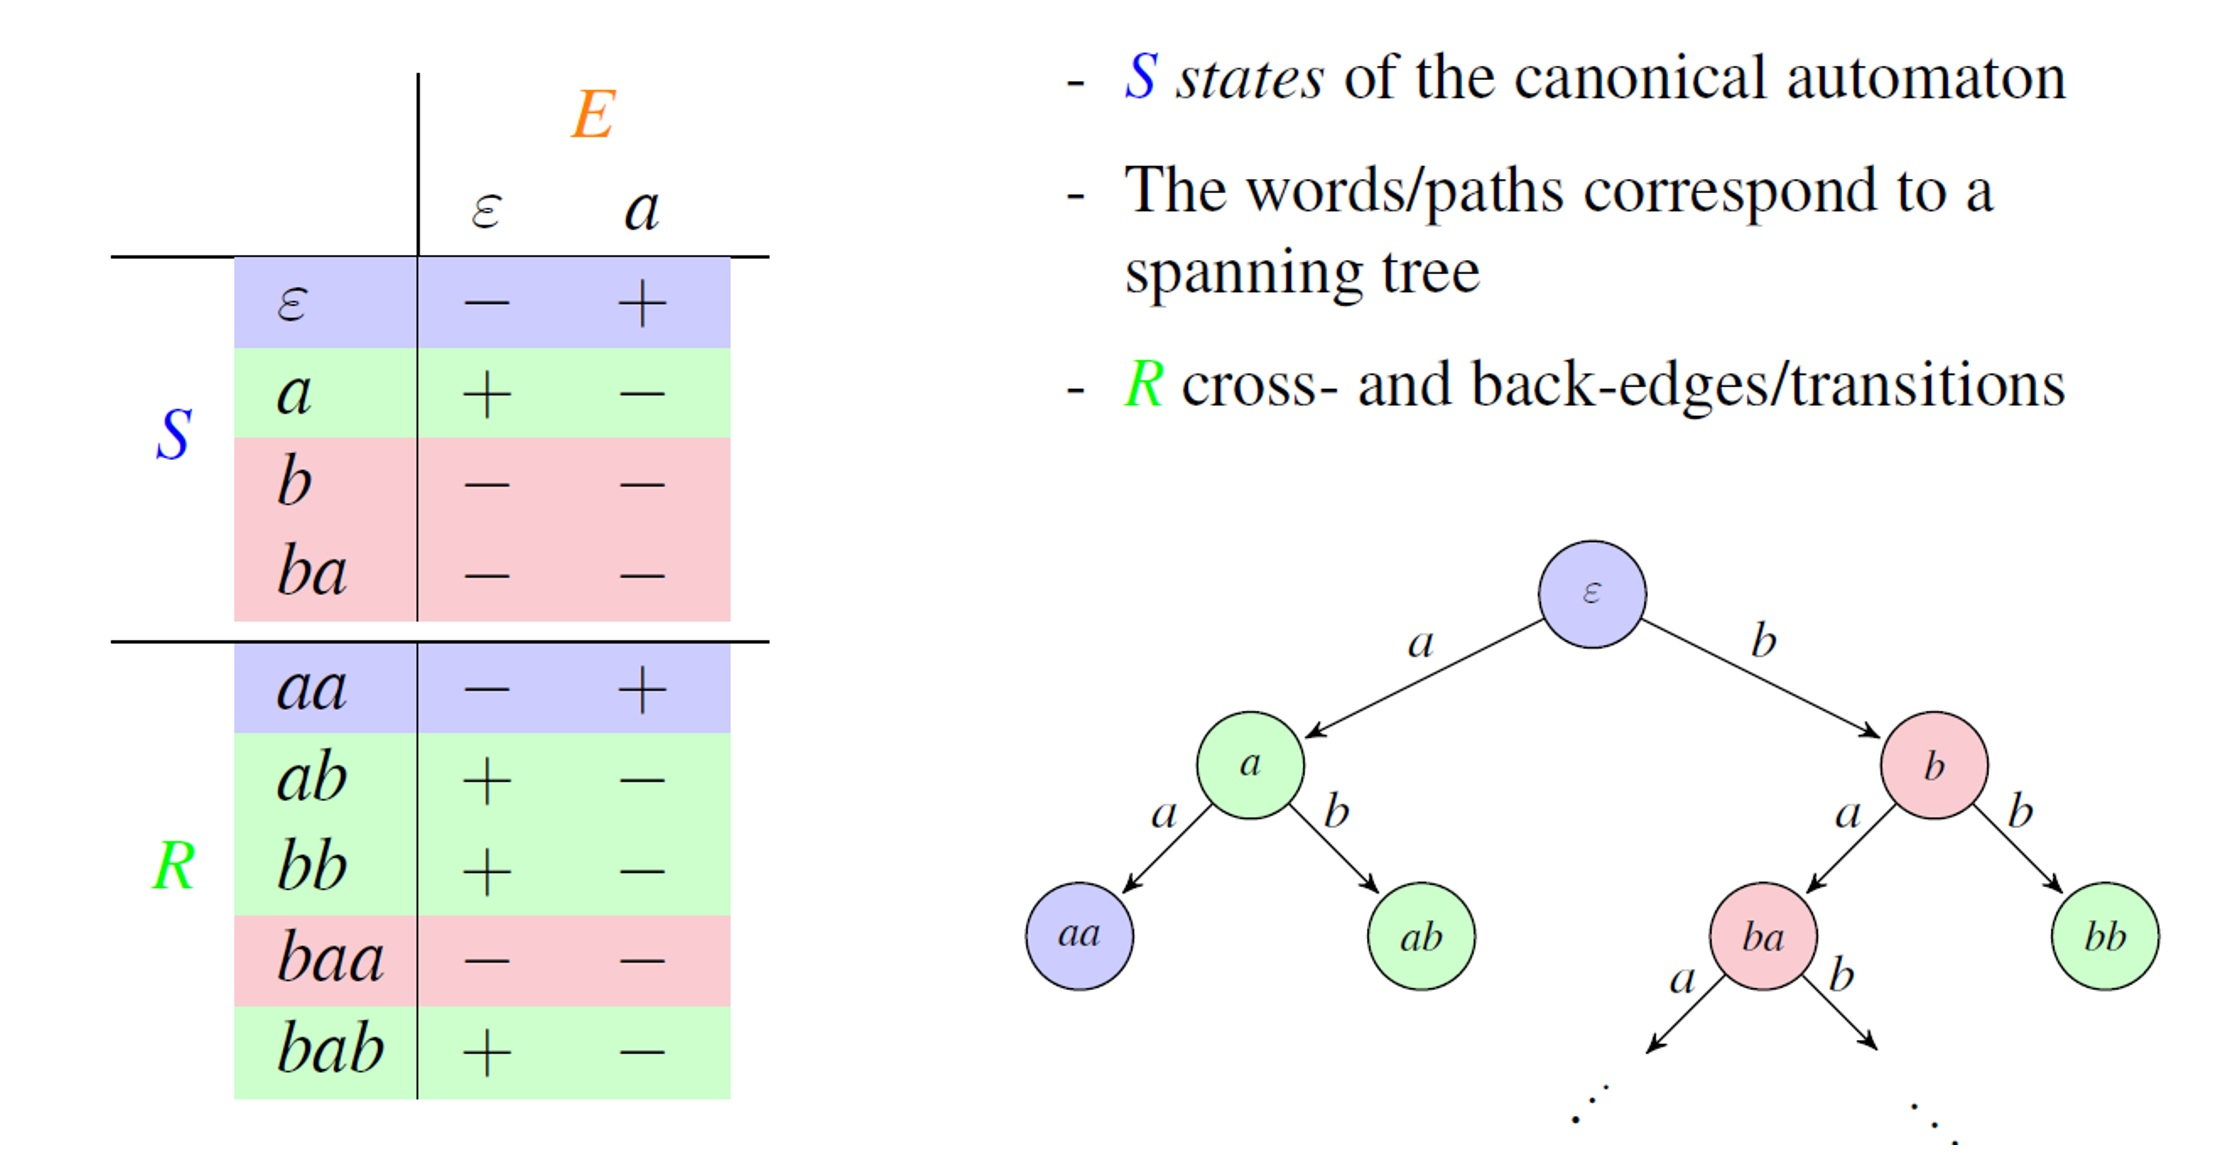
\includegraphics[width=\textwidth]{observationtable.jpg}
\end{center}

}

\frame{
\frametitle{Black Box Checking (Peled, Vardi \& Yannakakis)}

\begin{center}
 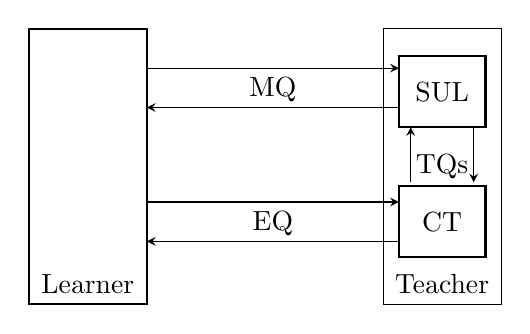
\begin{tikzpicture}[>=stealth]
            \draw [thick] (0,0) rectangle (1.5,3.5);
            \draw (4.5,0) rectangle (6,3.5) node[midway] {TQs};
            \draw [thick] (4.7,2.25) rectangle (5.8,3.15) node[midway] {SUL};
            \draw [thick] (4.7,0.6) rectangle (5.8,1.5) node[midway] {CT};
            \draw [->] (1.5,3) -- (4.7,3) node[midway,below] {MQ};
            \draw [<-] (1.5,2.5) -- (4.7,2.5);
            \draw [->] (1.5,1.3) -- (4.7,1.3) node[midway,below] {EQ};
            \draw [<-] (1.5,0.8) -- (4.7,0.8);
            \draw [->] (4.85,1.55) -- (4.85,2.25);
            \draw [<-] (5.65,1.55) -- (5.65,2.25);
            \node [below] at (0.75,0.5) {Learner};
            \node [below] at (5.25,0.5) {Teacher};
        \end{tikzpicture}
                \hspace{1 em}
        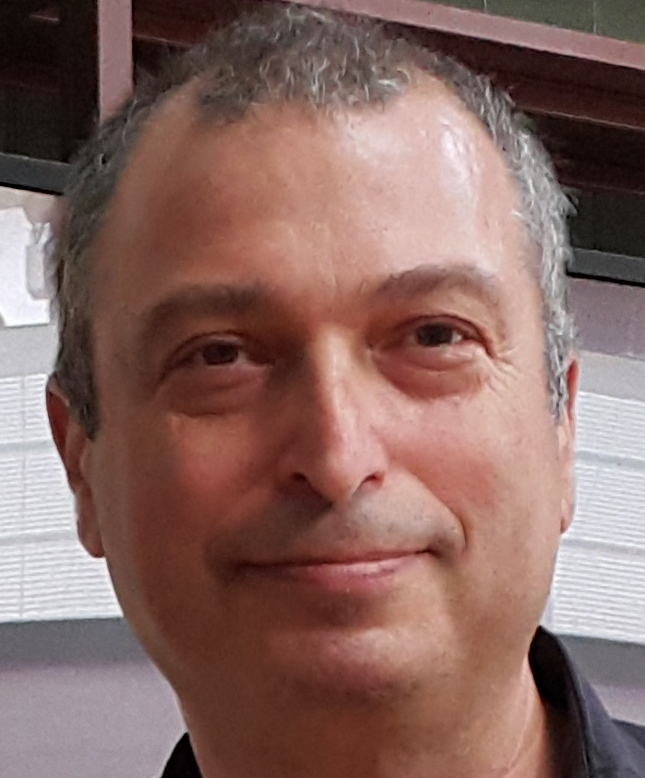
\includegraphics[width=1.2cm]{peled.jpg}
        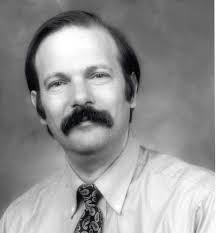
\includegraphics[width=1.35cm]{vardi.jpeg}
        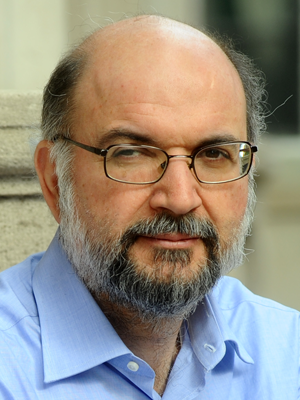
\includegraphics[width=1.1cm]{Yannakakis.png}
\end{center}
\red{Learner}: Formulate hypotheses\\
\red{Conformance Tester (CT)}: Test correctness hypotheses


\pause
\vspace{0.5em}
\red{Model learning and conformance testing two sides of same coin!}
}

\frame{
%\frametitle{LearnLib}

\begin{center}
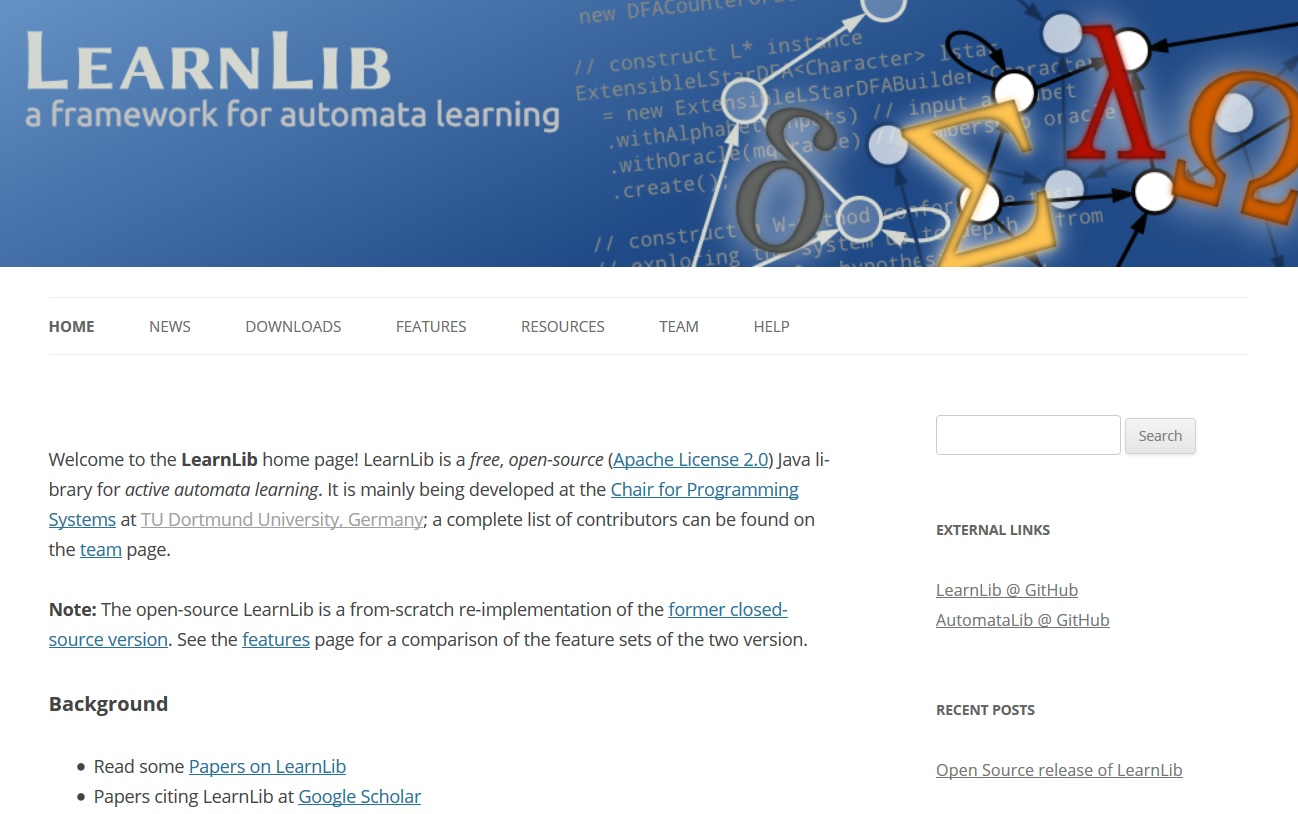
\includegraphics[width=.7\textwidth]{LearnLib.jpg}
    \hspace{1 em}
        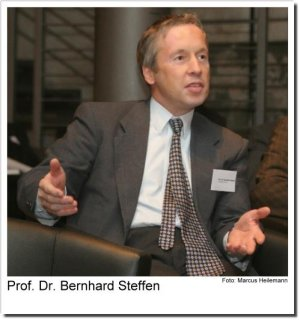
\includegraphics[width=2.5cm]{steffen.jpg}
\end{center}

Implements MAT framework for \red{DFAs}\  and \red{Mealy machines}
}


\frame{
\frametitle{A Theory of Mappers (FMSD, 2015)}

\begin{center}
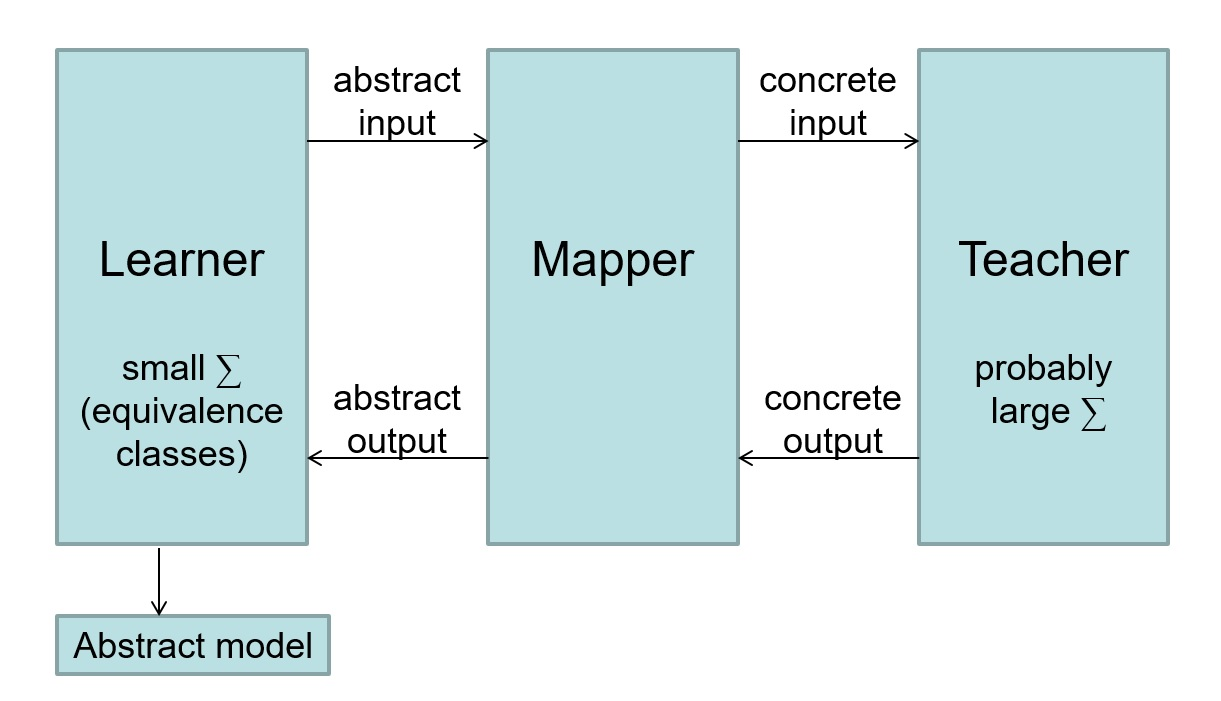
\includegraphics[width=.9\textwidth]{mappers.jpg}
\end{center}
}

\frame{
\frametitle{A Theory of Mappers (cnt)}

Formally, a mapper can be viewed as a transducer (deterministic Mealy machine). A mapper ${\cal A}$ induces an \red{abstraction operation\ } $\alpha_{\cal A}$ and a \red{concretization\ } operator $\gamma_{\cal A}$.

\begin{theorem}
%Suppose $\alpha_{\cal A}({\cal M})$ has no transitions with output $\perp$.
For a mapper ${\cal A}$ and nondeterministic Mealy machines ${\cal M}$ and ${\cal H}$,
$\alpha_{\cal A}({\cal M}) \leq {\cal H}$ iff
${\cal M} \leq \gamma_{\cal A}({\cal H})$.  \tiny{(modulo a minor technical condition)}
\end{theorem}
}

\section{Applications}

\frame{
	\frametitle{Our Research Method }
	
	\begin{center}
		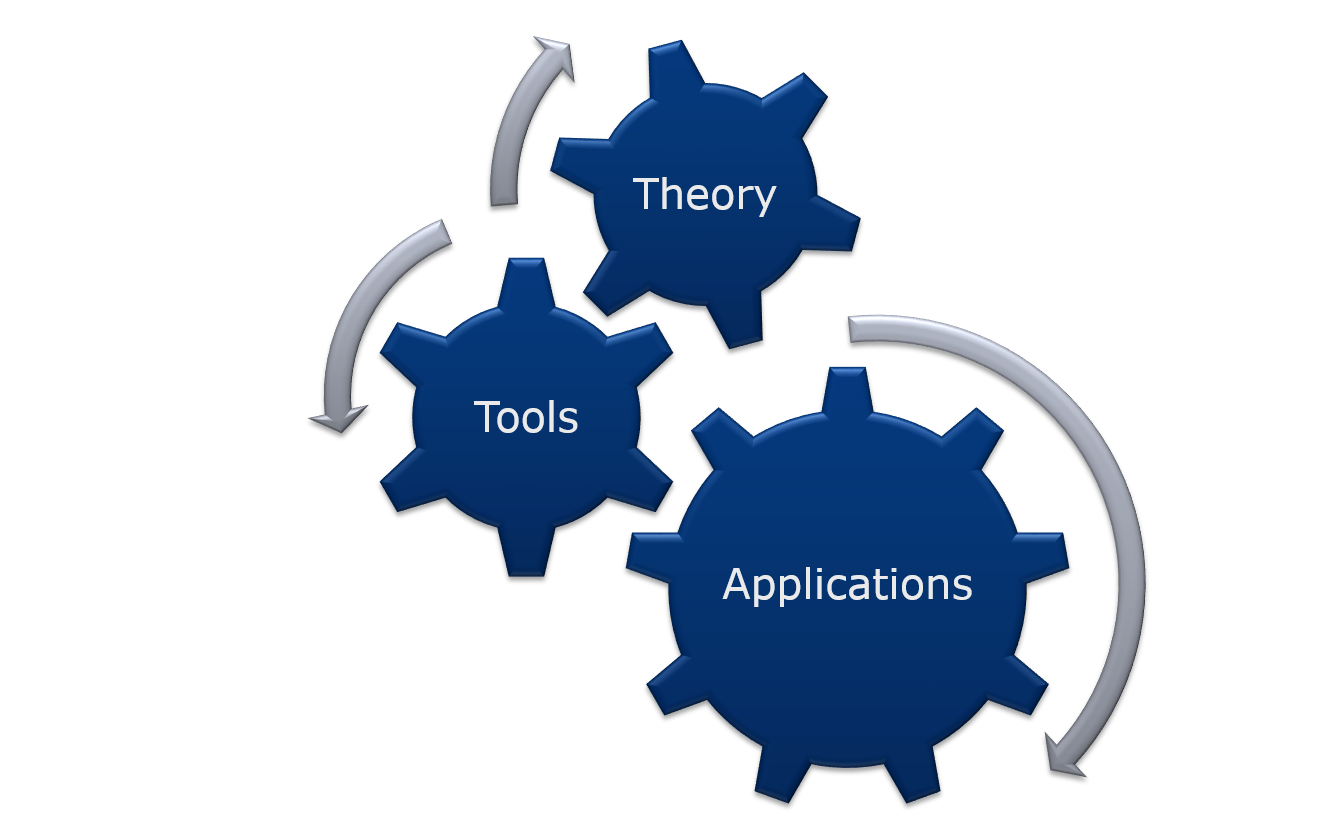
\includegraphics[width=.8\textwidth]{method.png}
	\end{center}
}

\frame{
\frametitle{EMV Protocol (Aarts et al, 2013)}

\begin{columns}
\begin{column}{0.5\textwidth}
    \begin{center}
     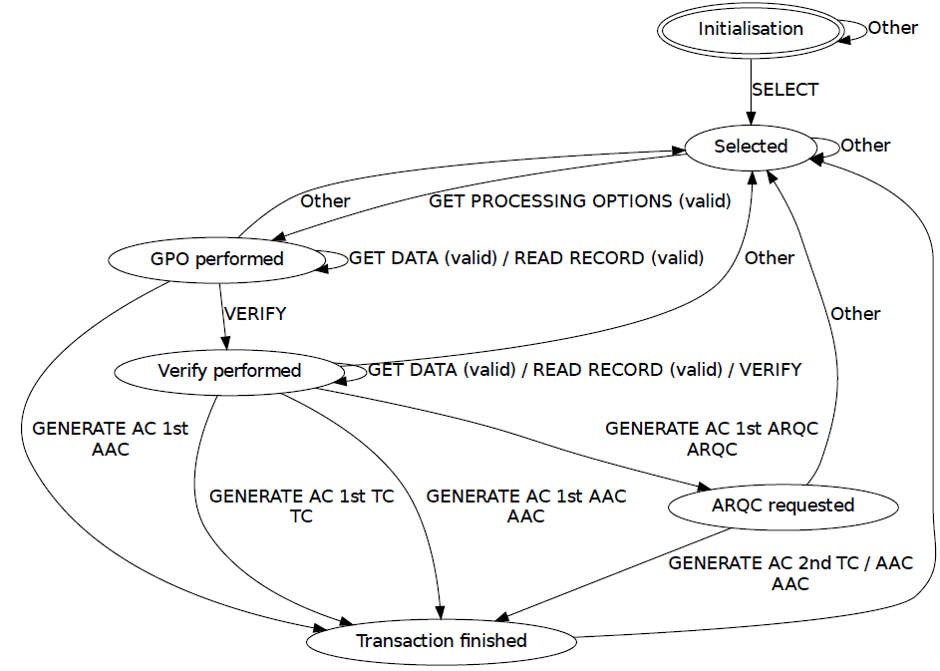
\includegraphics[width=\textwidth]{EMV.png}
     \end{center}
\end{column}
\begin{column}{0.5\textwidth}
{\small
\begin{itemize}
\item 
EMV = Europay/Mastercard/Visa
\item
Compatibility between smartcards and terminals 
\item
SEPA requires EMV compliance
\item
EMV standard has $>$700 pages
\item
Learning took at most 1500 membership queries, less than 30 minutes
\item
Useful for fingerprinting cards
\end{itemize}
}
\end{column}
\end{columns}
}
\frame{
\frametitle{E.dentifier2 (WOOT'14)}
\begin{center}
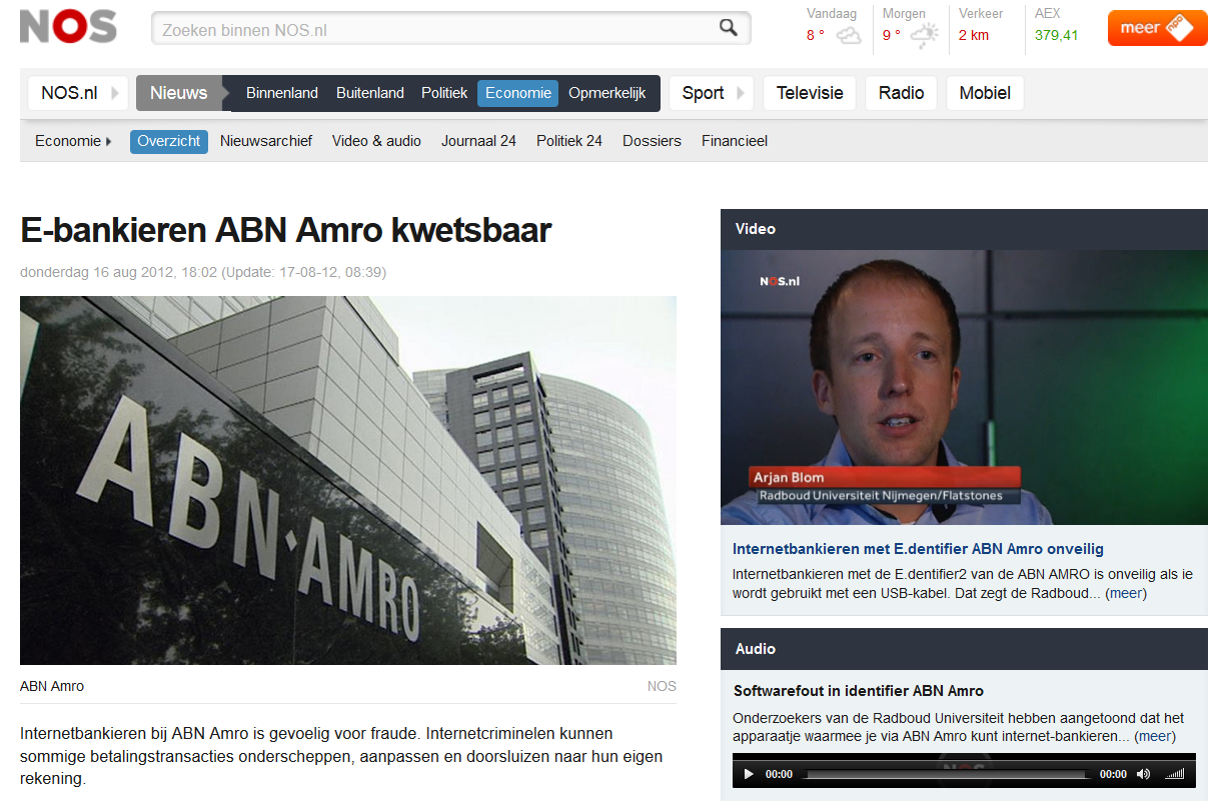
\includegraphics[width=.8\textwidth]{nosedentifier.png}
\end{center}
}

\frame{
\frametitle{State Machines for Old and New E.dentifier2}
\begin{center}
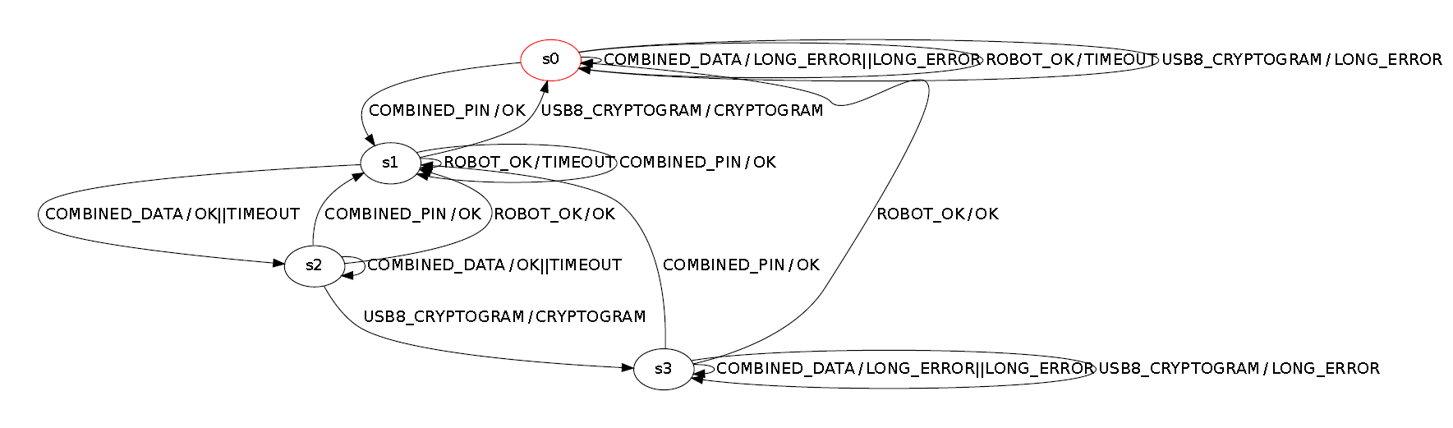
\includegraphics[width=.9\textwidth]{oldedentifier.png}

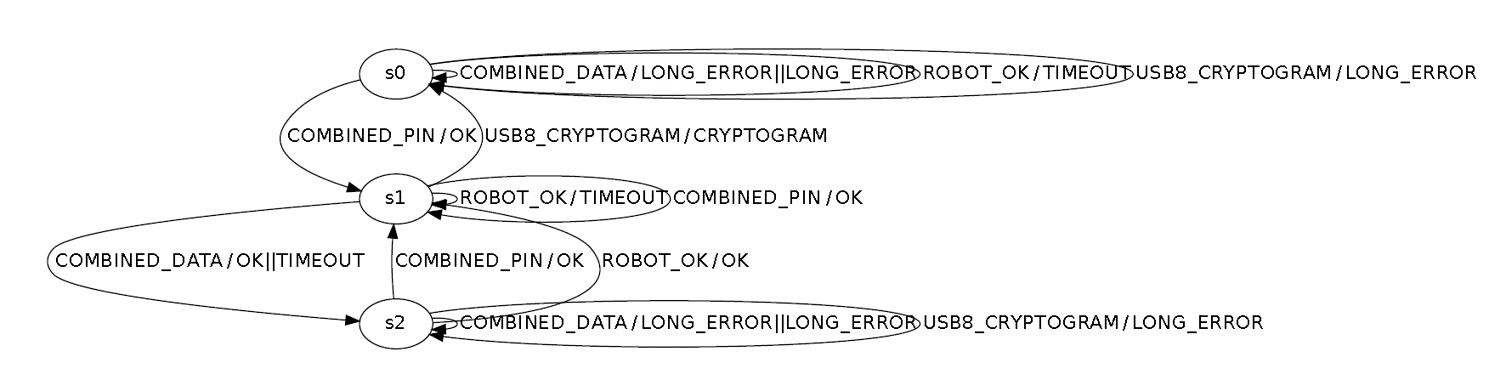
\includegraphics[width=.9\textwidth]{newedentifier.png}
\end{center}
}

\frame{
\frametitle{Bugs in Protocol Implementations}

\begin{columns}
\begin{column}{0.5\textwidth}  %%<--- here
    \begin{center}
     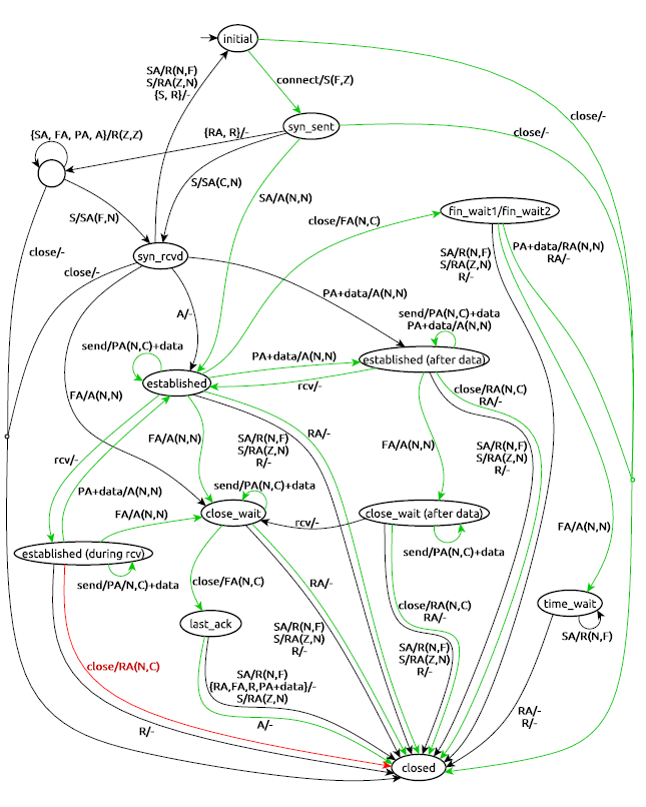
\includegraphics[width=0.9\textwidth]{TCPbug.png}
     \end{center}
\end{column}
\begin{column}{0.5\textwidth}
Standard violations found in implementations of major protocols: 
\begin{itemize}
\item
\blue{TLS}\  (Usenix Security'15)
\item 
\blue{TCP}\  (CAV'16)
\item
\blue{SSH}\  (Spin'17)
\end{itemize}
%
\pause
\red{These findings led to bug fixes in implementations.}
\end{column}
\end{columns}

}

\frame{
\frametitle{Learned Model for SSH Implementation}

\begin{center}
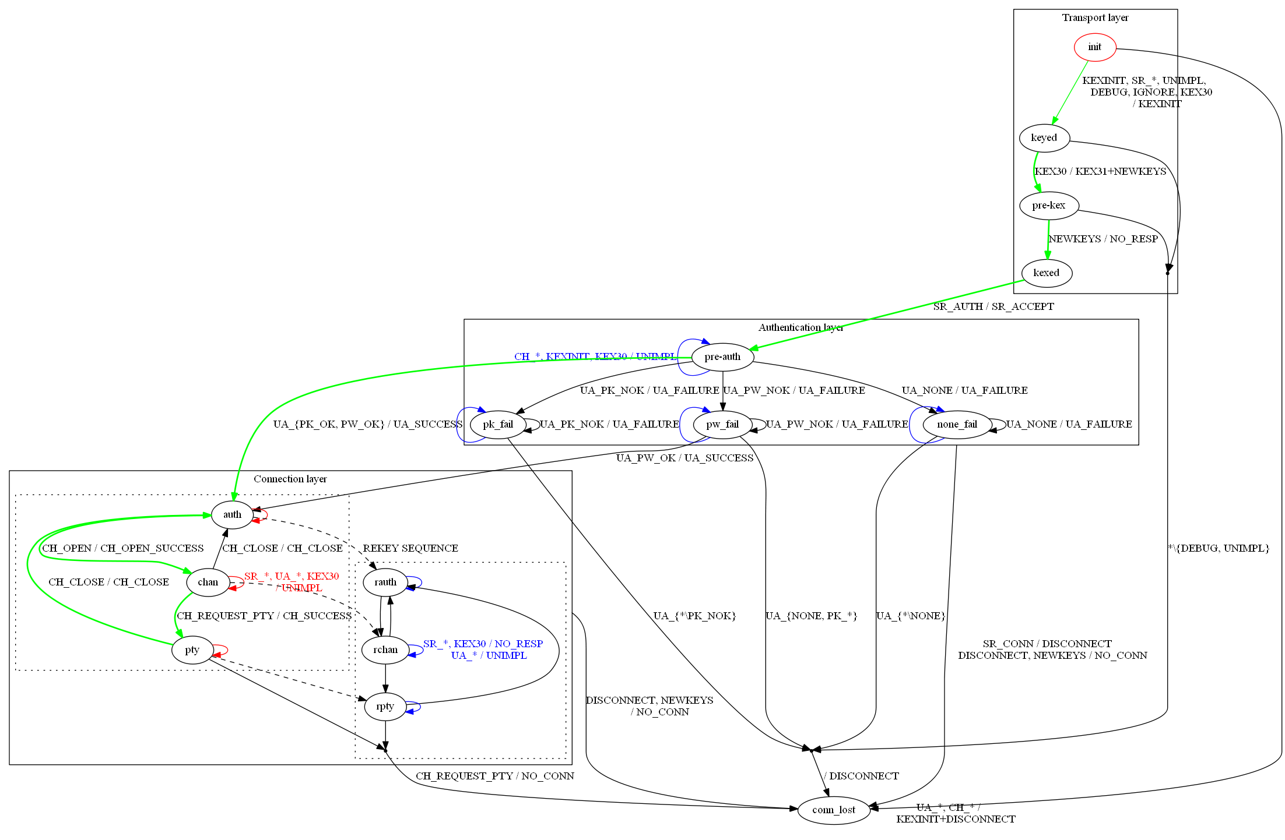
\includegraphics[width=\textwidth]{sshbug.png}
\end{center}
}
\frame{
\frametitle{SSH Model Checking Results}

\begin{center}
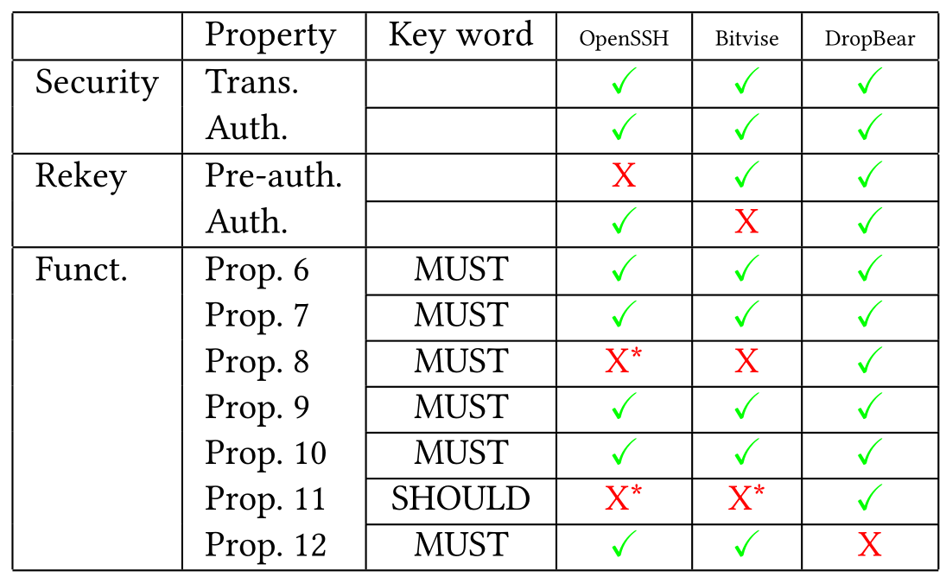
\includegraphics[width=\textwidth]{sshresults.png}
\end{center}
}

\frame{
\frametitle{Other Protocol Case Studies}
\begin{itemize}
\item
Session Initiation Protocol (SIP)
\item
Message Queuing Telemetry Transport (MQTT) protocol
\item
Quick UDP Internet Connections (QUIC) protocol
\item
WiFi
\item
IEC 60870-5-104 protocol
\item
...
\end{itemize}
}

\frame{
\frametitle{Lorentz Workshop}

\begin{columns}
\begin{column}{0.5\textwidth}  %%<--- here
    \begin{center}
     \includegraphics[width=0.9\textwidth]{lorentz.jpg}
     \end{center}
\end{column}
\begin{column}{0.5\textwidth}
Participants from automata learning, model-based testing, cryptography, and security protocol implementation. 

\vspace{0.5em}
Working groups on e.g.,
   \begin{itemize}
   \item 
   WiFi
   \item
   side channels in TLS
   \item
   LTE
   \end{itemize}
\end{column}
\end{columns}
}

\frame{
	\frametitle{Engine Status Manager in Oc\'{e} Printer (ICFEM'15)}
	
	\begin{center}
		\includegraphics[width=.6\textwidth]{Oceprinter.png}
	\end{center}
	
	Can we learn models of realistic printer controllers?
	
	\pause
	\vspace{1 em}
	\red{Potential applications:} regression testing, generation of new implementations
}


\frame{
	\frametitle{Conformance Testing Becomes the Bottleneck!}
	
	No existing conformance testing methods (W, Wp, HSI, ADS, UIOv, P, H, SPY,..) was able to find counterexamples for some hypotheses models of the printer software. We had to develop a new \red{hybrid ADS}\  method, based on work of Lee \& Yannakakis.
	
	\begin{center}
		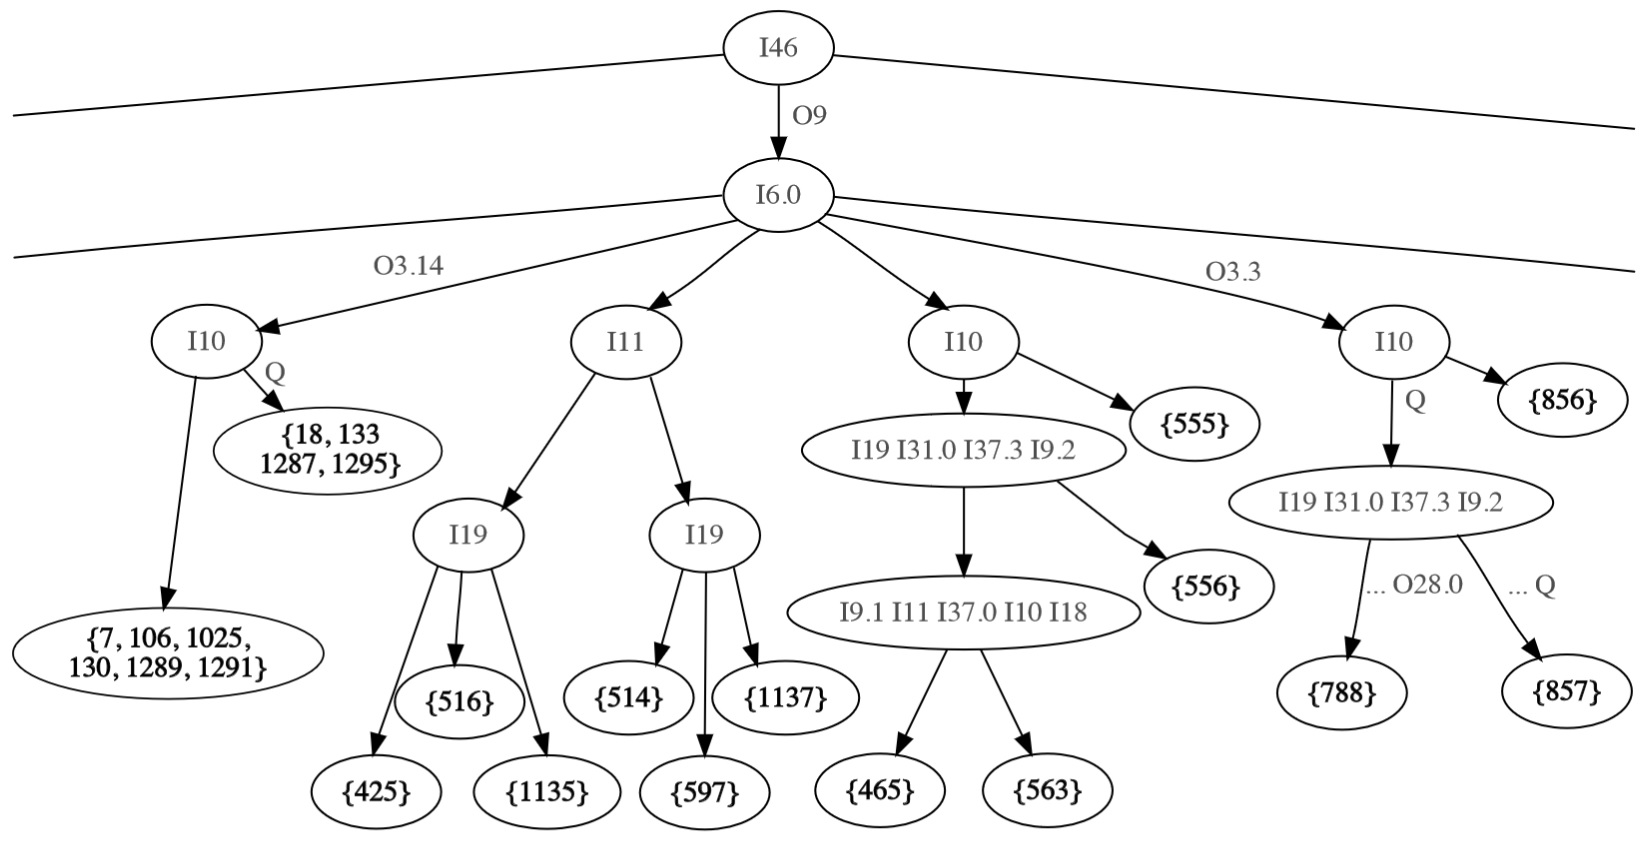
\includegraphics[width=.8\textwidth]{ADS.jpg}
	\end{center}
}


\frame{
	\frametitle{Mealy Machine for Engine Status Manager}
\begin{center}	
		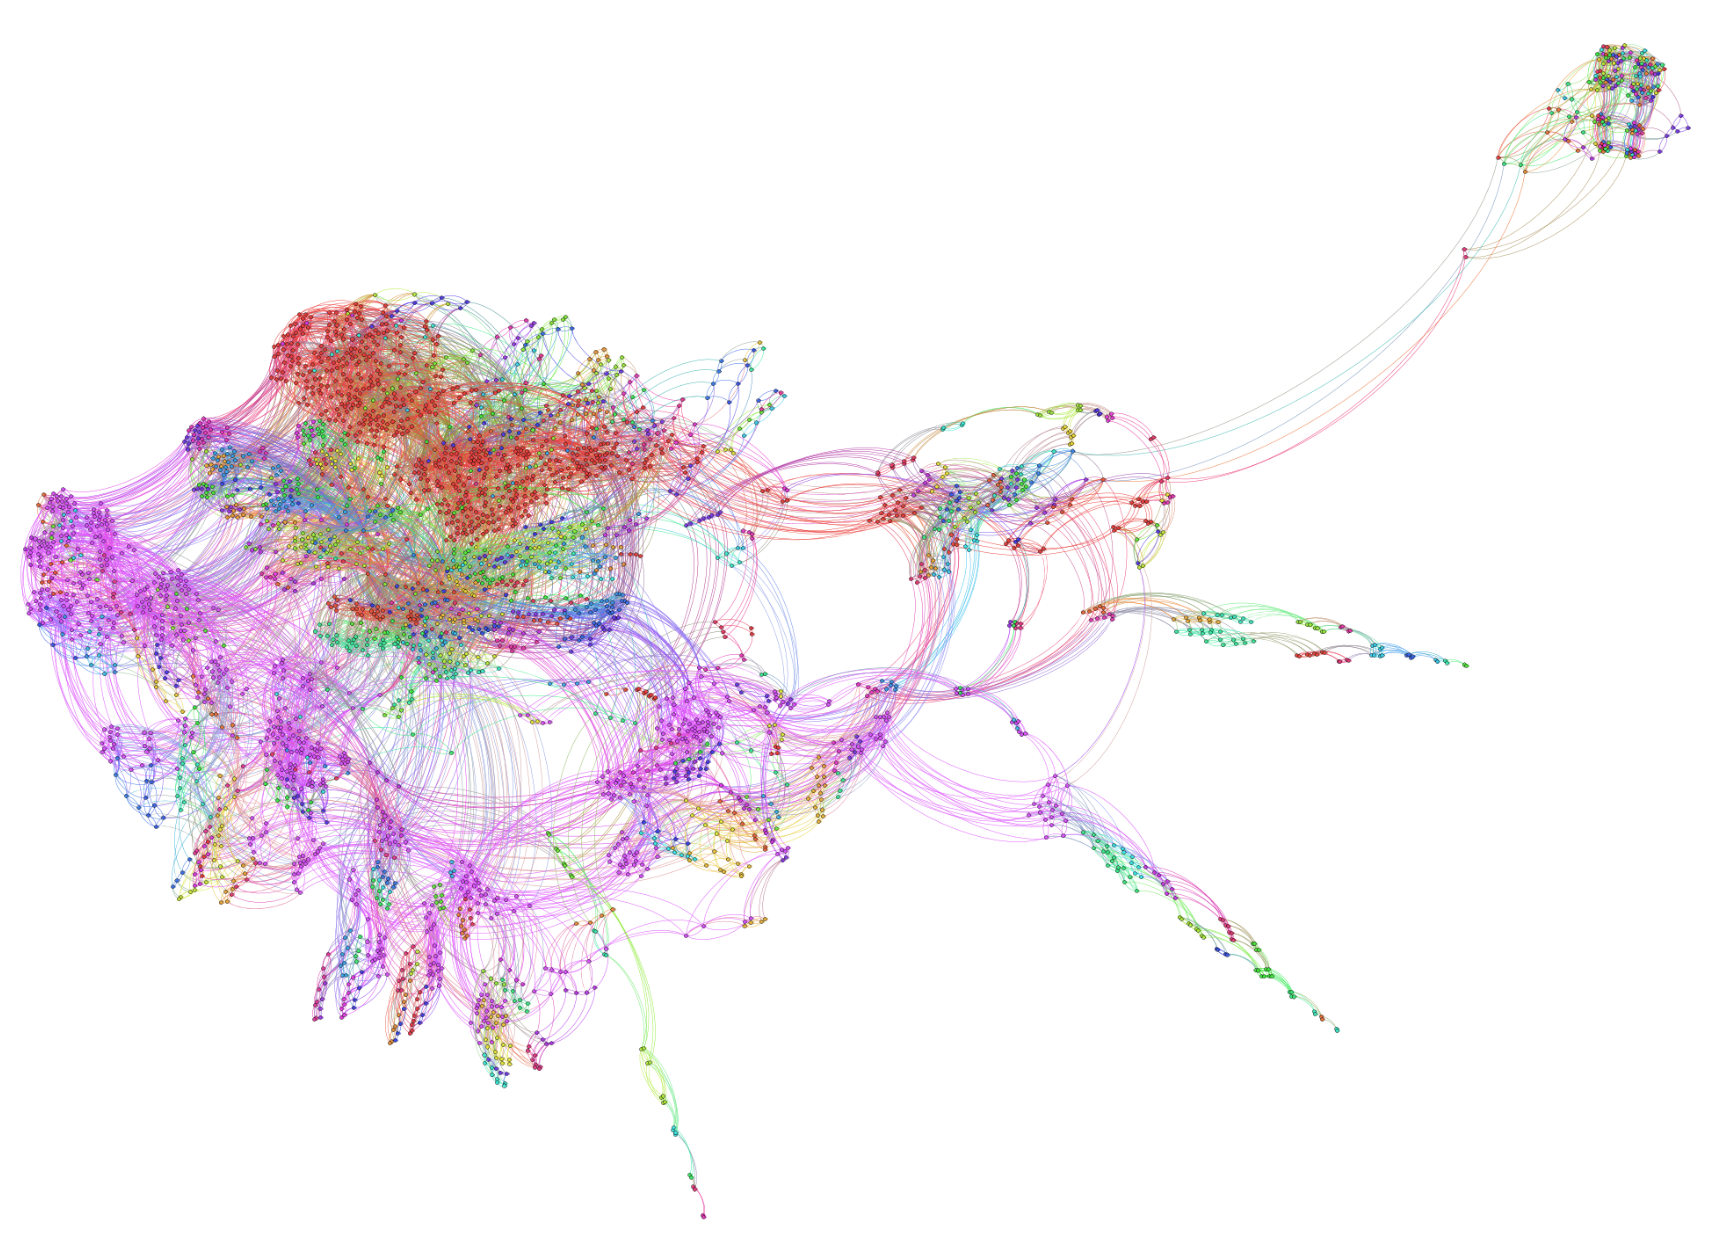
\includegraphics[width=0.8\textwidth]{ESM-manual.PNG}
\end{center}
}

\frame{
	\frametitle{Power Control Service from Philips Healthcare (iFM'16)}
	
	\begin{center}
		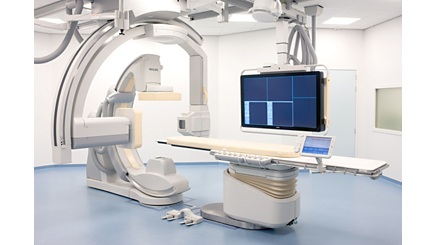
\includegraphics[width=.8\textwidth]{Xray.png}
	\end{center}
	
	Are legacy component and refactored implementation equivalent?
}

\frame{
	\frametitle{Refactoring Legacy Implementations}
	
	\begin{center}
		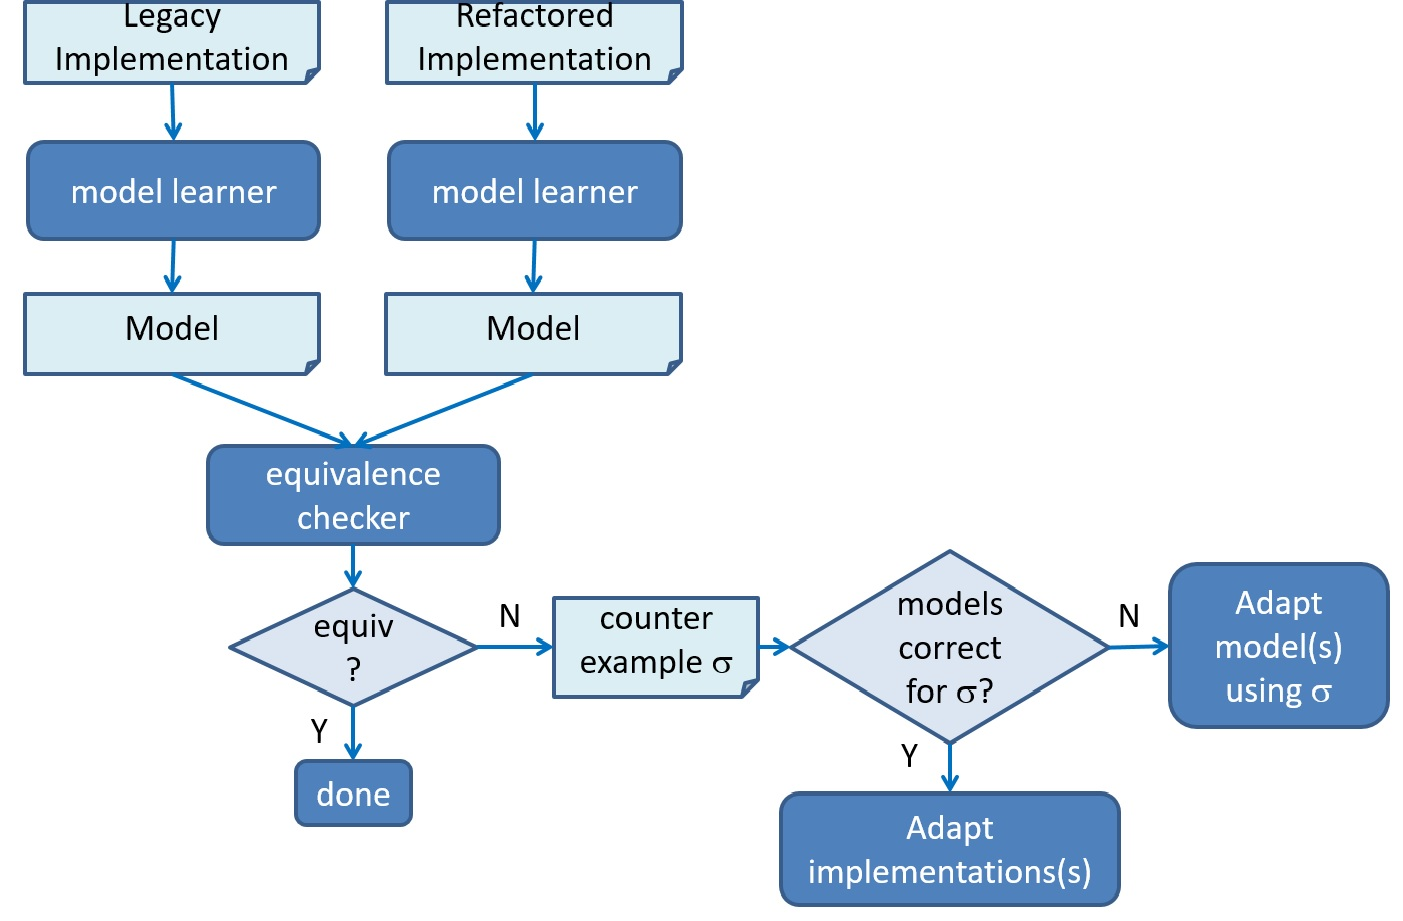
\includegraphics[width=.65\textwidth]{MethodeLegacy.jpg}
	\end{center}
	
	\pause
	\red{This approach allowed us to find several bugs in refactored implementations of power control service.}
	
	\pause
	\green{Learned model of a legacy component may also be used as runtime monitor for
		a refactored implementation (``lifelong learning'')}
}

\frame{
\frametitle{ASML Twinscan}

	\begin{center}
	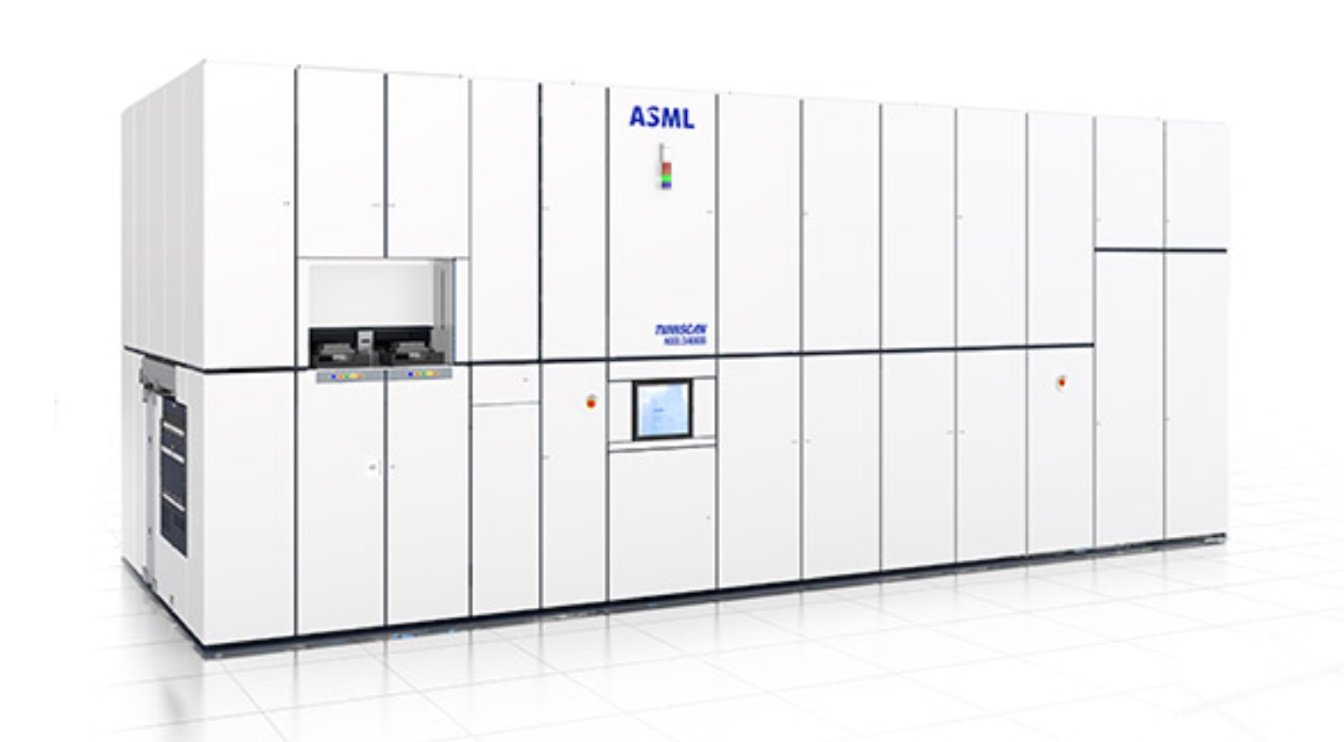
\includegraphics[width=\textwidth]{ASML-Feature.jpg}
\end{center}
}

\frame{
\frametitle{ASML Challenge}

Can active automata learning be used to support refactoring of legacy software at ASML?

\vspace{1 em}
ASML machines run on legacy software. Recent components have been designed using model-based techniques. Can we learn those?

\vspace{1 em}
Can we learn the hundreds of design and interface models
used for high level control of the wafer flow during lot operation?

\pause
\vspace{1 em}
\red{$\Rightarrow$ RERS @ TOOLympics'19}
}

\frame{
\frametitle{Results LearnLib on ASML Benchmarks}

\begin{center}
	\includegraphics[width=0.8\textwidth]{ASMLBenchmarks.jpg}
\end{center}

}

\section{Theory \& Tools for Model Learning}
\frame{
\frametitle{Benchmark Wiki \url{automata.cs.ru.nl}}

\begin{center}
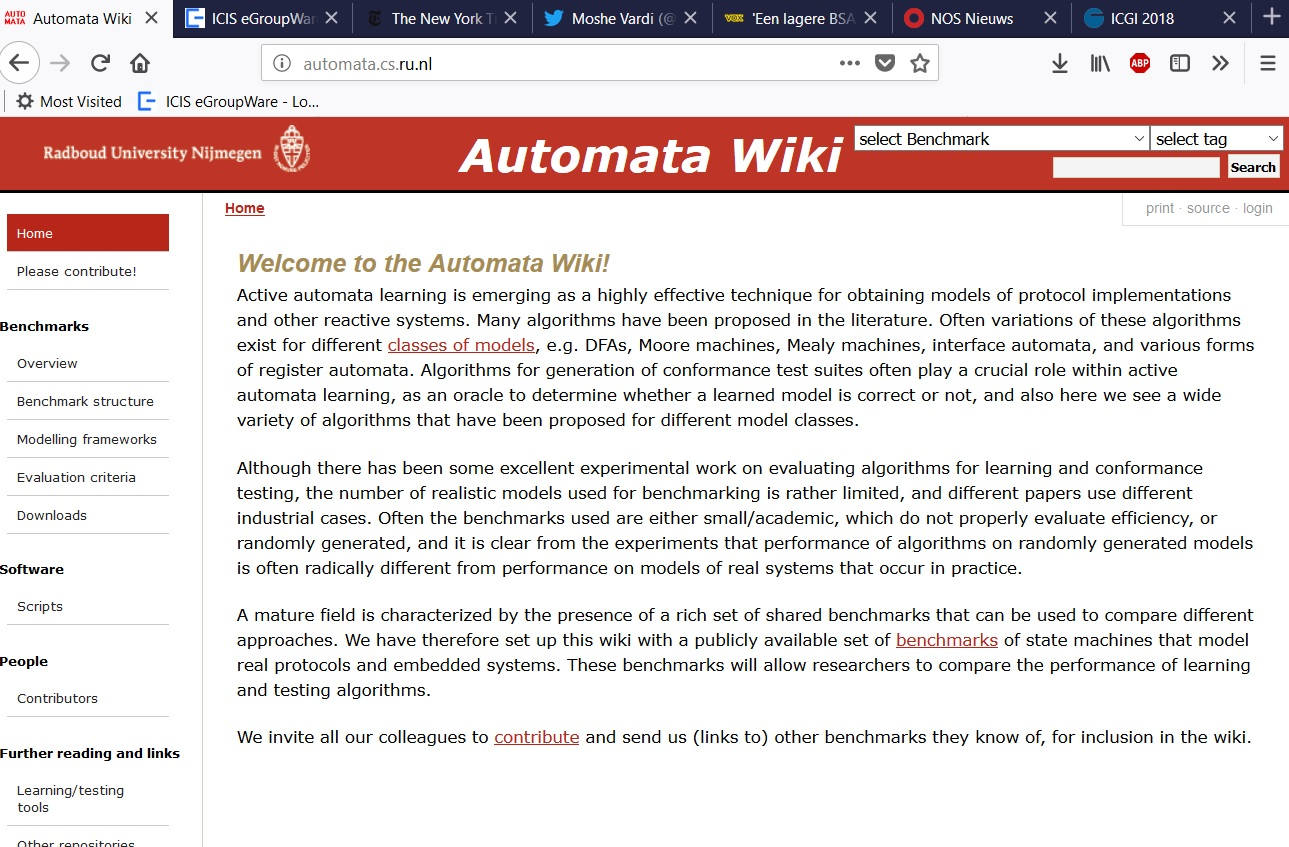
\includegraphics[width=.9\textwidth]{automatawiki.jpg}
\end{center}
}


\frame{
\frametitle{Benchmark Wiki \url{automata.cs.ru.nl}}

\begin{center}
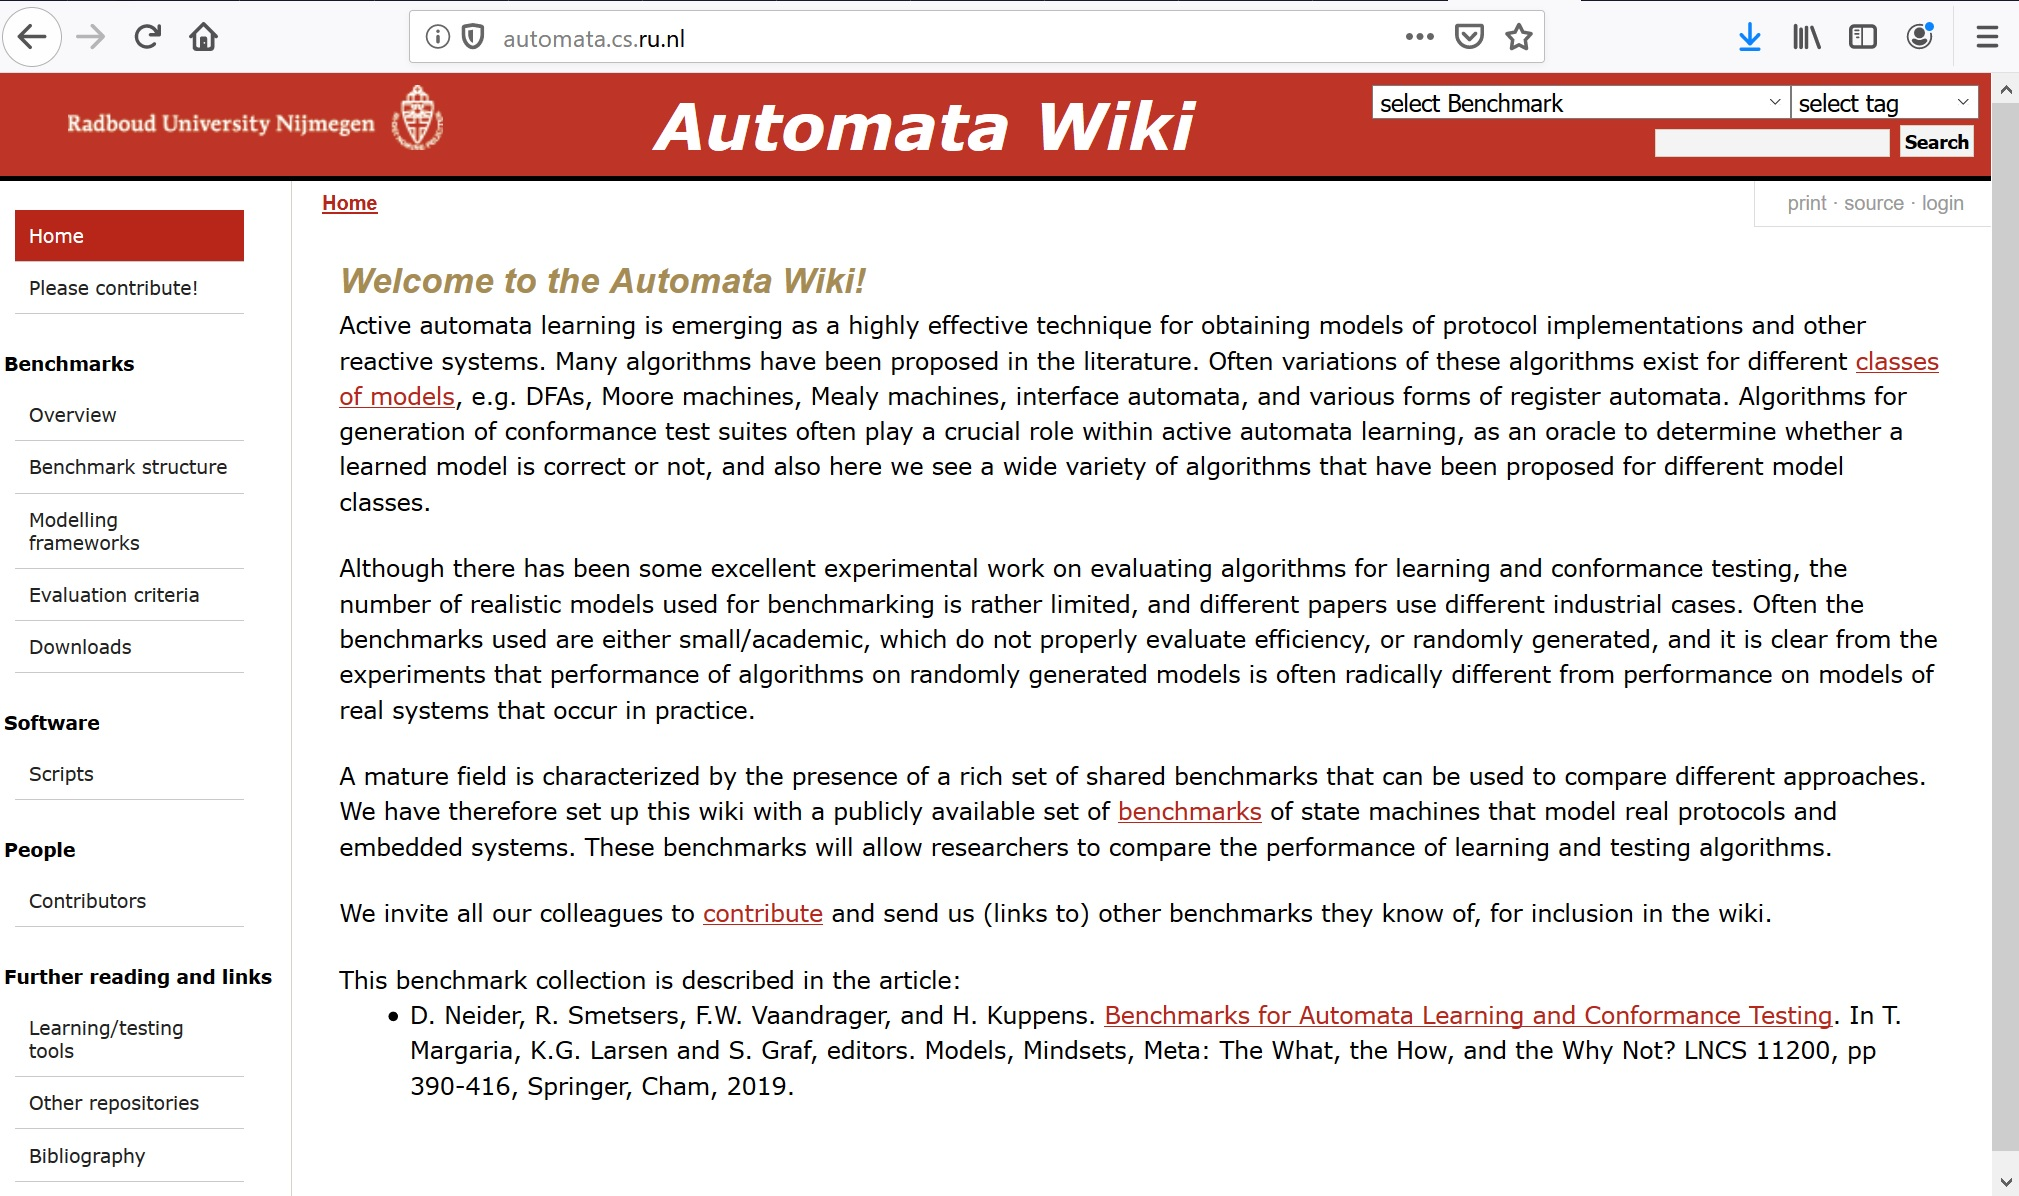
\includegraphics[width=.9\textwidth]{benchmarks.jpg}
\end{center}
}


\frame{
\frametitle{Benchmark Wiki: Supported Automata Frameworks}

\begin{center}
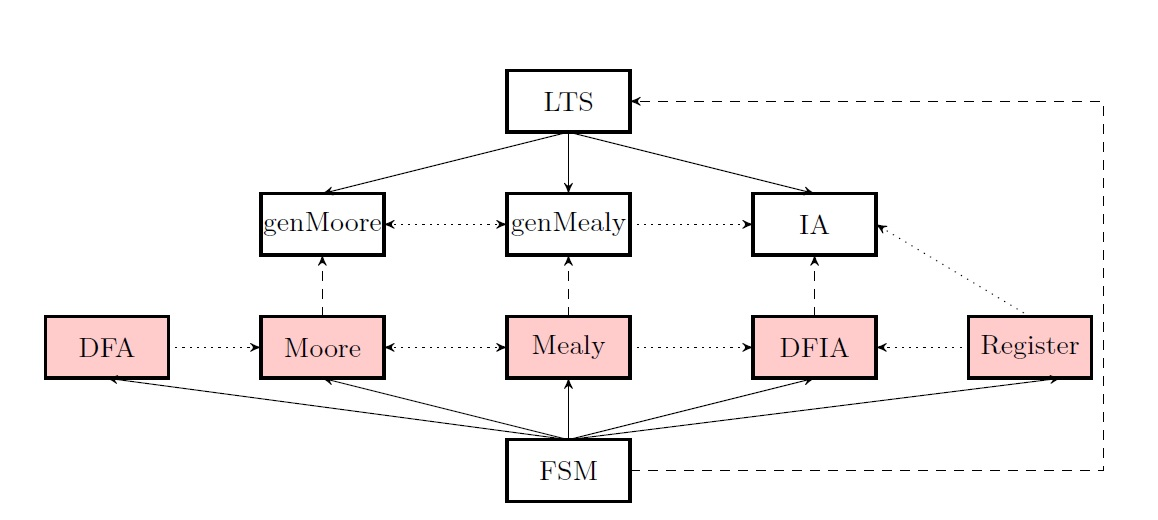
\includegraphics[width=\textwidth]{automataframeworks.jpg}
\end{center}
}


\frame{
\frametitle{Automata Wiki: Most Benchmarks are not that Big}

\begin{center}
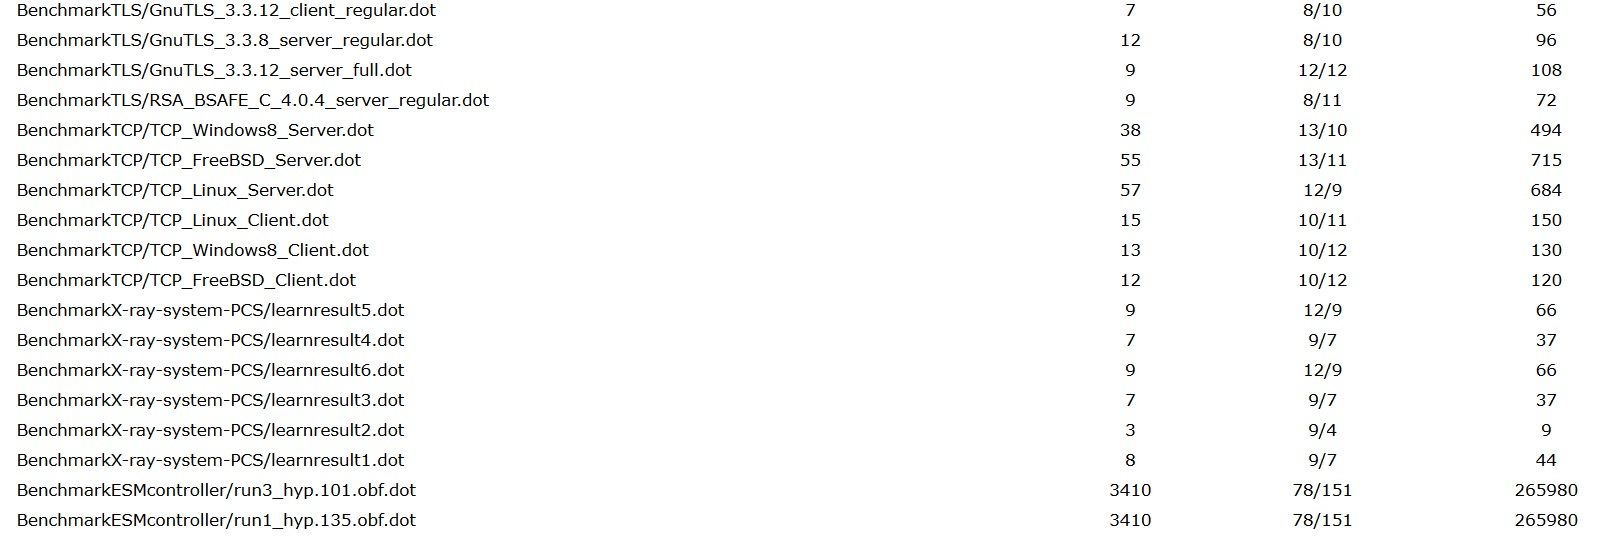
\includegraphics[width=\textwidth]{benchmarksize.jpg}
\end{center}
}


\frame{
	\frametitle{Learning Product Automata (Moerman, ICGI'18)}
	
	Consider a Moore machine with outputs $O_1 \times O_2$
	
	\begin{center}
		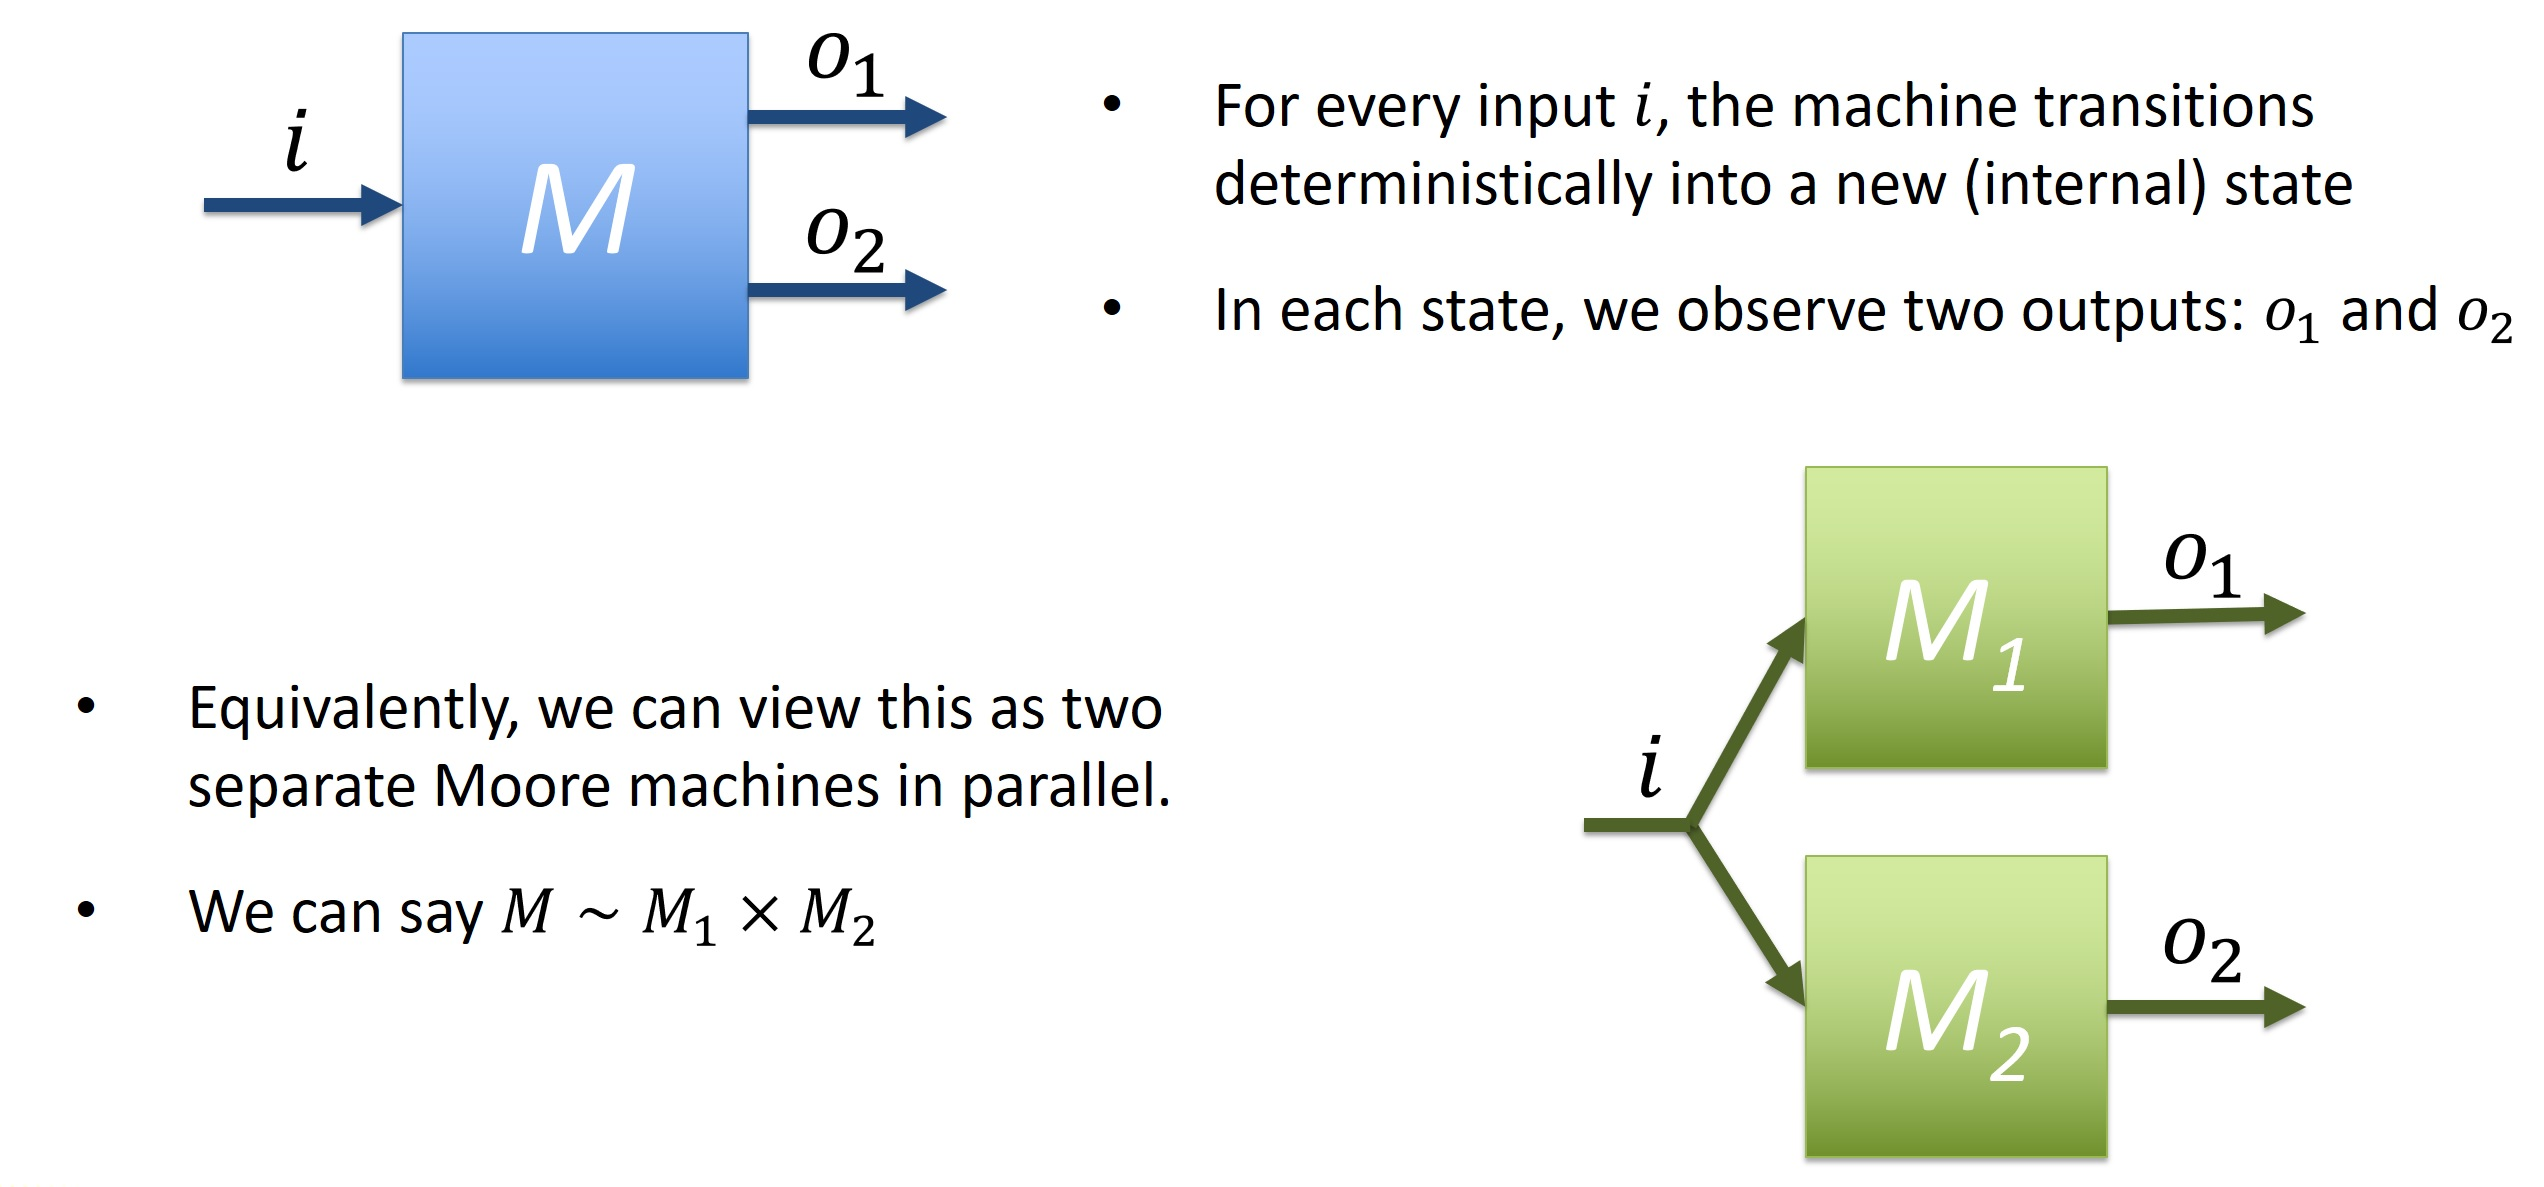
\includegraphics[width=\textwidth]{productautomata.jpg}
	\end{center}
}

\frame{
	\frametitle{An Example from Rivest \& Schapire}
		
	\begin{center}
		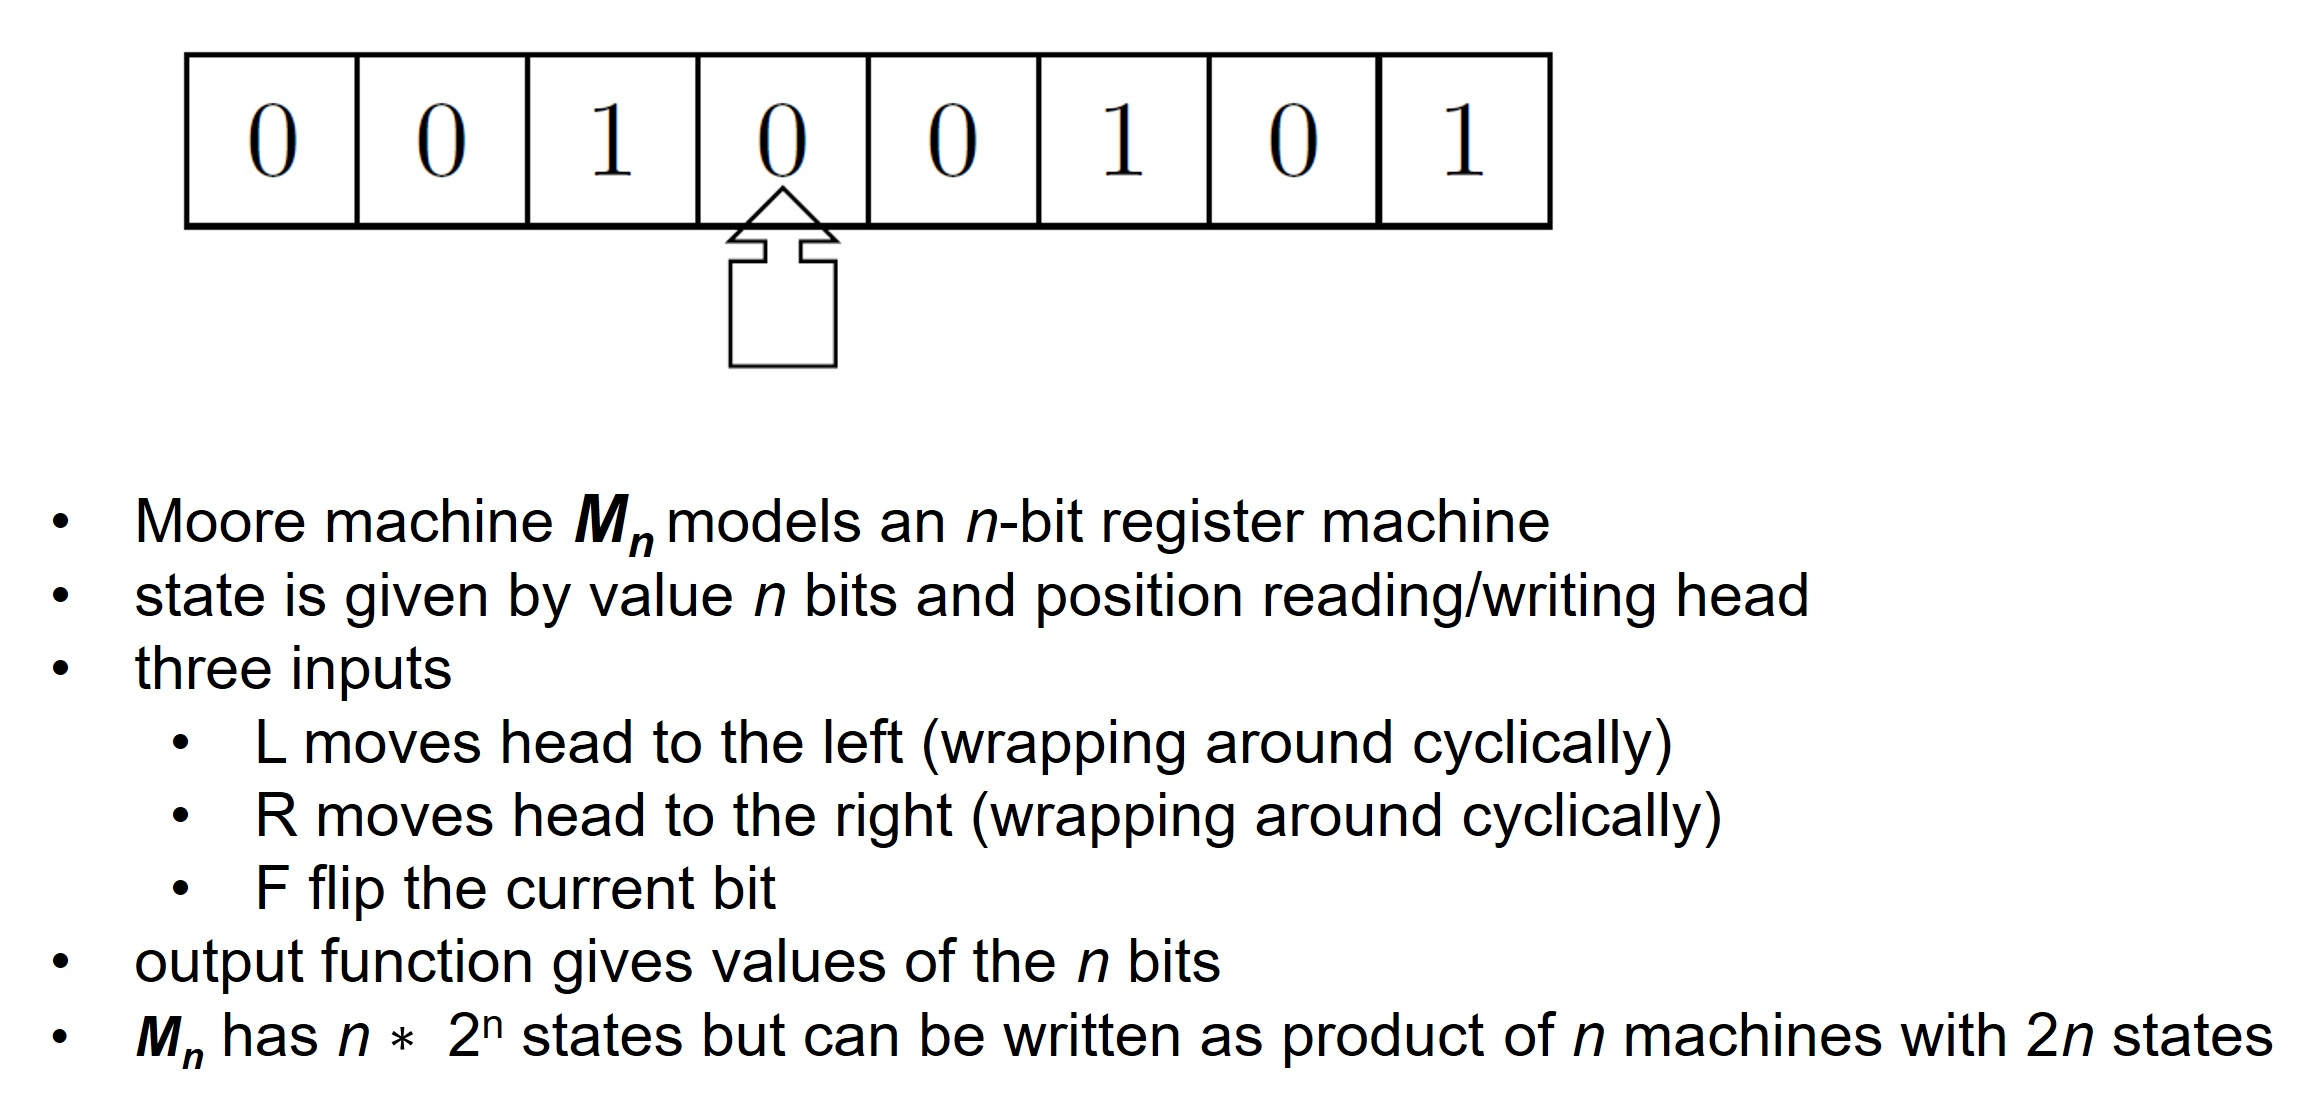
\includegraphics[width=\textwidth]{rivestschapire.jpg}
	\end{center}
}

\frame{
	\frametitle{Experimental Evaluation}
	
	\begin{center}
		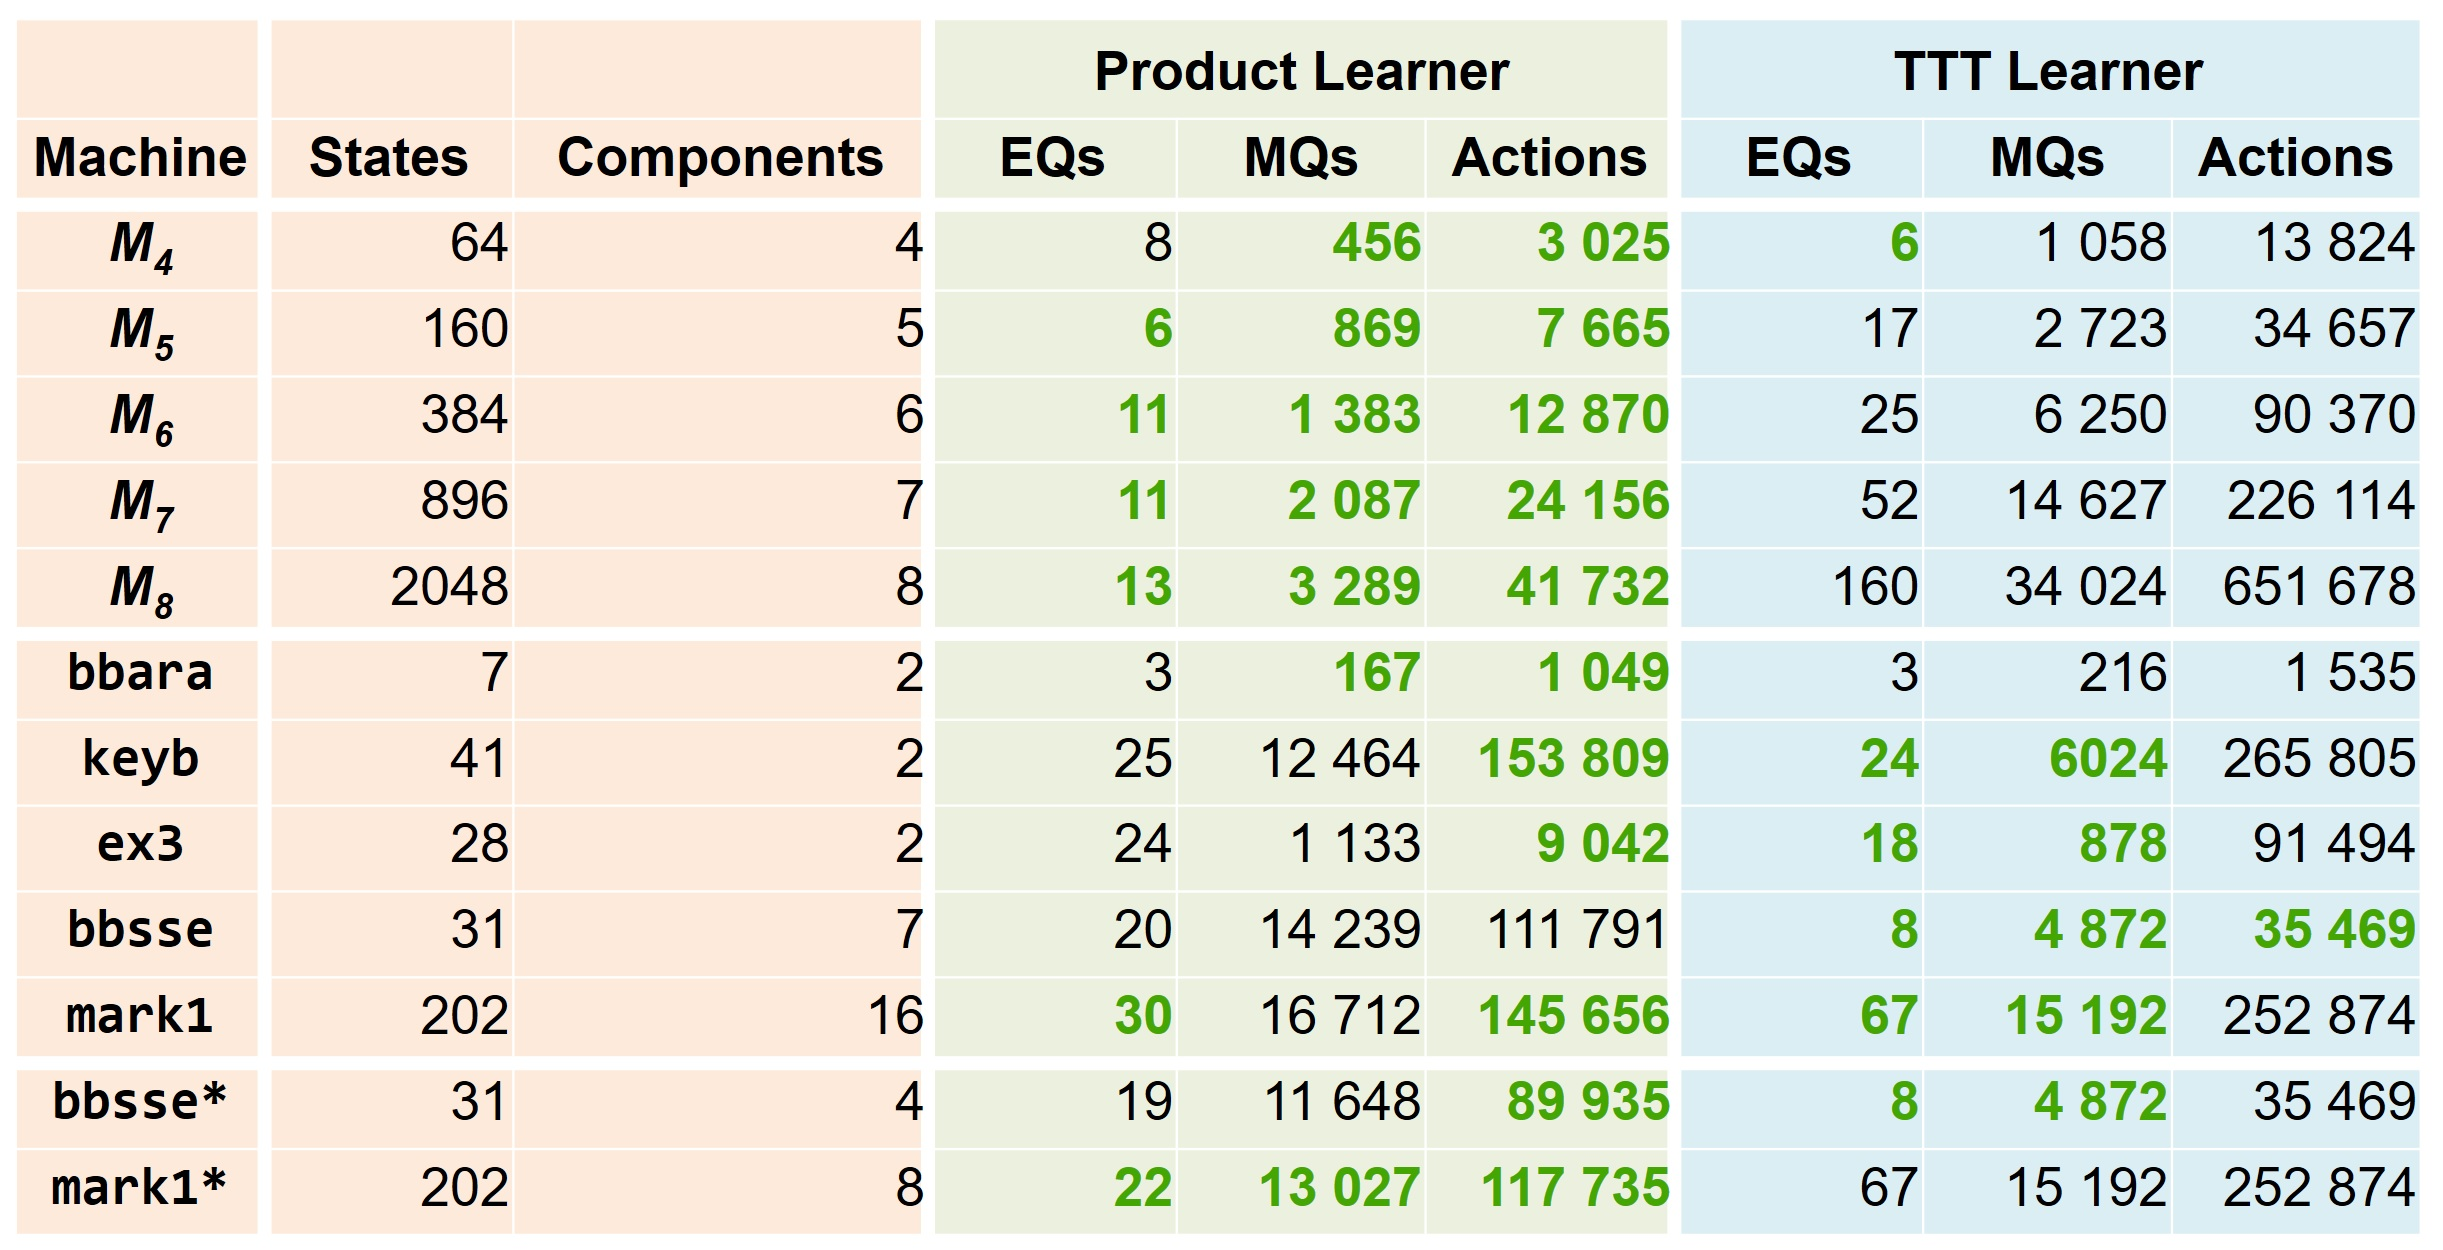
\includegraphics[width=\textwidth]{experimentsproduct.jpg}
	\end{center}
}

\frame{
\frametitle{Register Automata}

Actions may carry data parameters that may be stored in registers:
\begin{center}
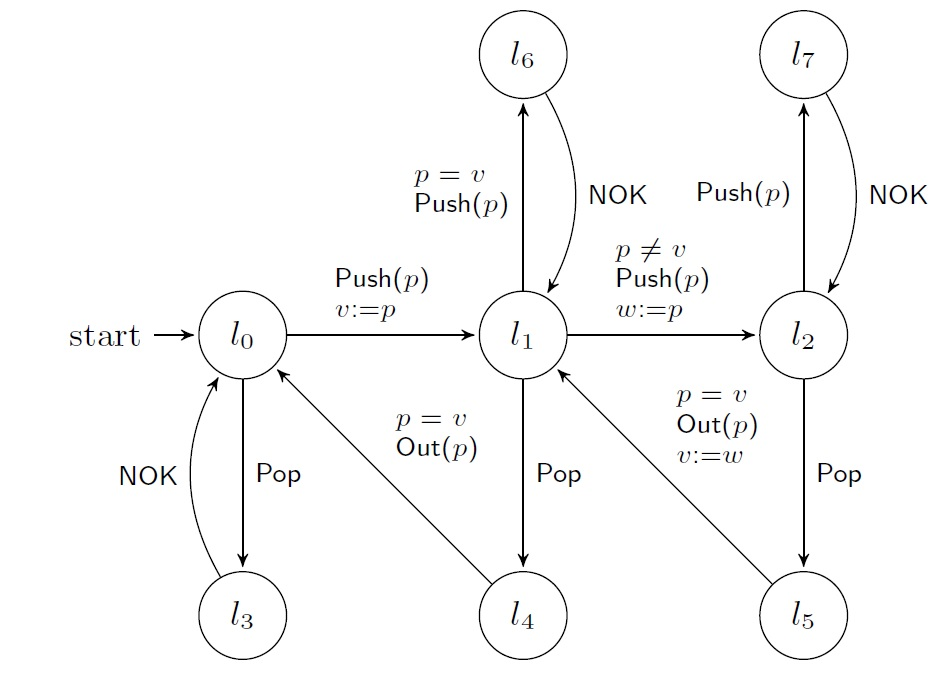
\includegraphics[width=.8\textwidth]{fifoset.jpg}
\end{center}
}

\frame{
\frametitle{Data Types}

Register automata may be parametrized by a \red{(relational) structure}: a pair $\tuple{\domain, \binrelations}$
where $\domain$ is an unbounded domain
% \todobj{Do we need it to be unbounded?}
of \red{data values}, and
$\binrelations$ is a collection of \red{relations\ } on $\domain$. 

\vspace{0.5em}
Examples of simple structures include:
\begin{itemize}
\item
  $\tuple{\mathbb{N}, \{=\} }$, the natural numbers with
  equality; 
\item
  $\tuple{\mathbb{R}, \{ <\} }$, the real numbers with inequality:
  this structure also allows one to express equality between elements.
\end{itemize}
Transition guards are conjunctions of negated and unnegated relations from $\binrelations$.
}

\frame{
\frametitle{Learning Tools for Register Automata}
\begin{itemize}
\item 
\blue{Tomte}, Radboud University, can only handle $\tuple{\mathbb{N}, \{=\} }$
\item
\blue{LearnLib}, TU Dortmund, can only handle $\tuple{\mathbb{N}, \{=\} }$
\item
\blue{RALib}, Uppsala/Dortmund, can handle some richer structures
\end{itemize}

}
\frame{
\frametitle{TCP Protocol Case Study (FMICS-AVoCS'17)}

\begin{center}
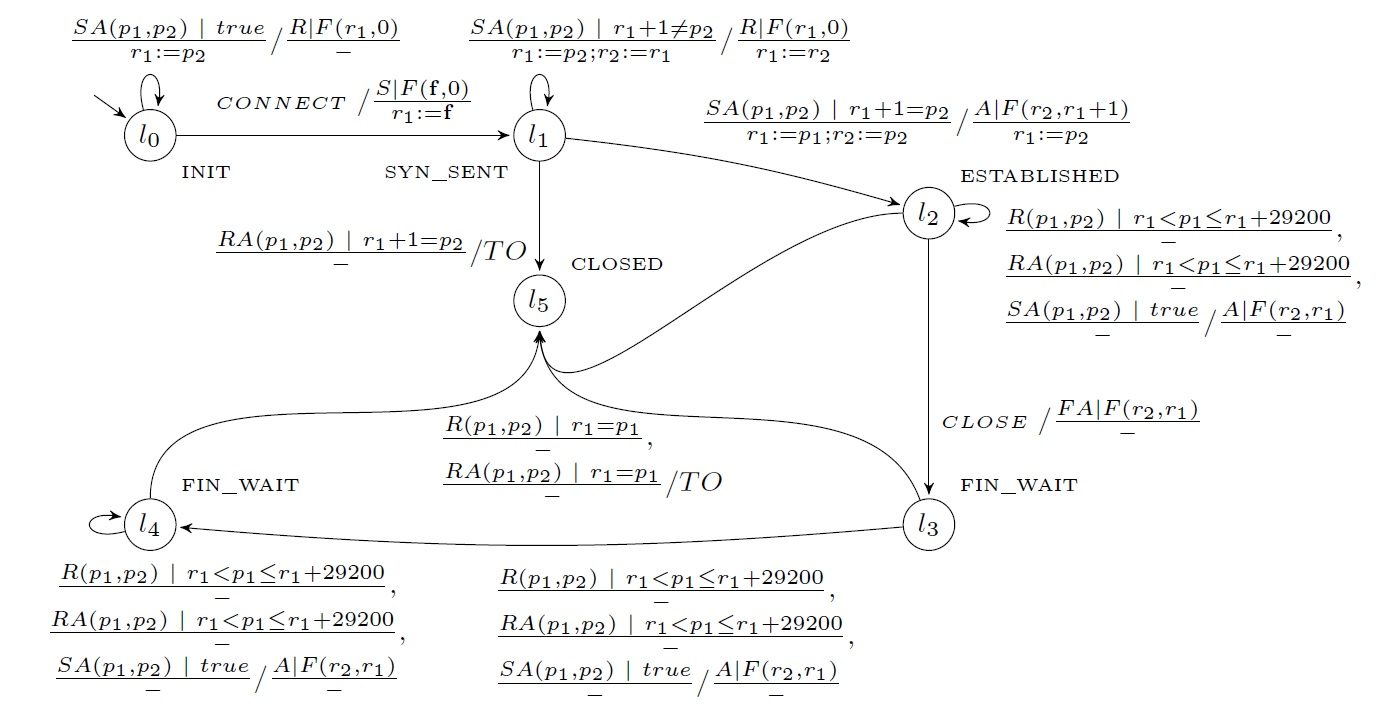
\includegraphics[width=\textwidth]{TCPlinux.jpg}
\end{center}
\pause
\red{These findings led to bug fix in Linux TCP implementation!}
}


\frame{
\frametitle{Limits of Black-box Learning?}

\begin{itemize}
\item 
Model learning is an highly effective bug finding technique
\pause
\item
... but it has some serious scalability problems
\pause
\item
\red{Can we use white-box information while preserving the extensionality of black-box models?}
\end{itemize}

\pause\red{Yes, we can!}
}

\frame{
\frametitle{Fuzzing}

\begin{center}
	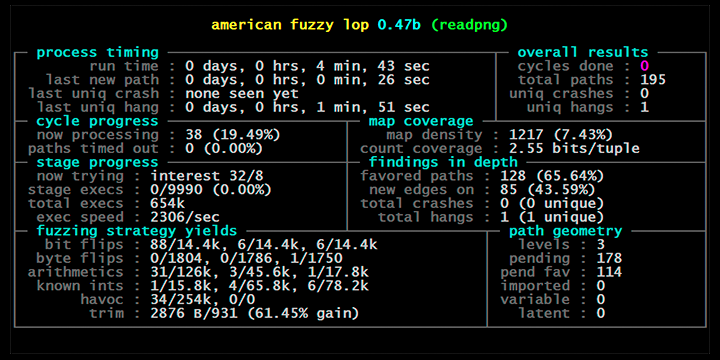
\includegraphics[width=.7\textwidth]{afl_screen.png}
\end{center}
By combining LearnLib, hybrid ADS testing, and the \red{American fuzzy lop fuzzer (AFL)},
my group, together with colleagues from Delft, won the RERS 2016 challenge. 
}

\frame{
\frametitle{Taint Analysis}

\begin{center}
\includegraphics[width=.8\textwidth]{ants.jpg}
\end{center}
}


\frame{
\frametitle{Taint Analysis}

\begin{itemize}
\item
White-box technique for code analysis
\item
Instruments code to track input values
\item
Many tools focus on specific vulnerabilities, e.g.\ buffer overflows and sql injections
\item
Usually implemented using Dynamic Binary Analysis, e.g.\ Valgrind
\item
We use Python library from Pygmalion tool from Andreas Zeller et al.
\end{itemize}
}

\frame{
\frametitle{What Does Pygmalion Do For Us?}

\begin{center}
\includegraphics[width=\textwidth]{taintedtrace.jpg}
\end{center}

\pause
\red{Potential of exponential gains during learning!}
}
\frame{
\frametitle{Architecture RAlib Tool for Learning Register Automata}

\begin{center}
 \includegraphics[width=\textwidth]{ralib.jpg}
\end{center}
}

\frame{
\frametitle{Tree Oracle}

\begin{center}
 \includegraphics[width=0.6\textwidth]{SDT.jpg}
\end{center}
}

\frame{
\frametitle{Ongoing Work}

Replace tree oracle in RAlib by a version that uses taint analysis.

\vspace{2cm}
\pause
\red{First prototype finished (for integers with equality)}
}

\section{Conclusions and Future Work}
\frame{
\frametitle{Conclusions}
Active automata learning is emerging as a highly effective bug-finding technique,
and (very) slowly becoming a standard tool in the toolbox of the software engineer.

\vspace{1 em}
But \red{much\ } further research is needed!
}

\frame{
\frametitle{Future Work}
\begin{enumerate}
\item
Further improvement of black-box learning/testing algorithms for FSMs	
\item
Explore combinations of black-box and white-box learning
\item
Develop algorithms for models with time and probabilities
\item
Refactoring of legacy software is potentially excellent application domain
\end{enumerate}
}





\end{document}
